% LaTeX-Layout for report or thesis at FH Aachen
% Author: Paul Kalhorn
% structure adopted from Sven Hinz (FH Aachen)  (https://github.com/SvenHinz) and Jennifer Eisele (https://de.overleaf.com/latex/templates/fh-aachen-one-sided-report-or-thesis-fh-aachen-vorlage-abschlussarbeit-einseitig/tvxhzskxjhct)


% This document is optimized for a onesided layout.
% It is possible to change the layout to a twosided document by changing the class to \documentclass[twoside,openright,12pt,a4paper]{scrreprt} and adjusting the geometry \usepackage[left=2.5cm,right=1.5cm,top=2.5cm,bottom=2.5cm]{geometry}
% But there might be problems with footer and header.
% ihead needs to be changed from \ihead[\sffamily \bfseries \upshape \headmark]{\sffamily \bfseries \upshape \headmark} to \ihead[]{}

\documentclass[oneside,openright,12pt,a4paper]{scrreprt}

% Paket für Umlaute (für Deutsch):
\usepackage[utf8]{inputenc}       % Cross Platform
\usepackage[T1]{fontenc}          % Korrekte Umlaut-Kodierung im PDF (Copy-Paste)
\usepackage{hyperref}   %links in TOC
\hypersetup{
    colorlinks=false, %set true if you want colored links of references and crossreferences
    linktoc=all,     %set to all if you want both sections and subsections linked
}

\usepackage[ngerman]{babel}       % Sprache: Deutsch
\usepackage[german=quotes]{csquotes} % \enquote{} für deutsche Anführungszeichen
\usepackage[ddmmyyyy]{datetime}
\renewcommand{\dateseparator}{.}
\usepackage{amsmath}
\usepackage{amssymb}
\usepackage{makeidx}
\usepackage{graphicx}
\usepackage{epstopdf}
\usepackage{blindtext}
\usepackage[left=2.0cm,right=2.0cm,top=2.5cm,bottom=2.5cm]{geometry}

\newcommand\tab[1][1cm]{\hspace*{#1}}

\author{Kacper Cömlek}

\usepackage[automark,plainheadsepline,headsepline]{scrlayer-scrpage}
\usepackage{color}
\usepackage{setspace}
\usepackage[scaled]{helvet}
\usepackage[numbers,sort&compress,square]{natbib} %this bibstyle uses numbers, which are sorted (increasing) and summarized eg. 104,105,106 --> 104-106
\usepackage{longtable}
\usepackage{listings}
\usepackage{xcolor}
\usepackage{rotating}
\usepackage{pdfpages}
\usepackage{caption}
\usepackage{subcaption}
\usepackage{booktabs}
\usepackage[export]{adjustbox}
\usepackage{svg}

% code
\definecolor{codegreen}{rgb}{0,0.6,0}
\definecolor{codegray}{rgb}{0.5,0.5,0.5}
\definecolor{codepurple}{rgb}{0.58,0,0.82}
\definecolor{backcolour}{rgb}{0.95,0.95,0.92}

\lstdefinestyle{mystyle}{
    backgroundcolor=\color{backcolour},
    commentstyle=\color{codegreen},
    keywordstyle=\color{magenta},
    numberstyle=\tiny\color{codegray},
    stringstyle=\color{codepurple},
    basicstyle=\ttfamily\footnotesize,
    breakatwhitespace=false,
    breaklines=true,
    captionpos=b,
    keepspaces=true,
    numbers=left,
    numbersep=5pt,
    showspaces=false,
    showstringspaces=false,
    showtabs=false,
    tabsize=2
}

\lstset{style=mystyle}

% Python code style
\lstdefinestyle{python}{
    language=Python,
    backgroundcolor=\color{backcolour},
    commentstyle=\color{codegreen},
    keywordstyle=\color{magenta},
    numberstyle=\tiny\color{codegray},
    stringstyle=\color{codepurple},
    basicstyle=\ttfamily\footnotesize,
    breakatwhitespace=false,
    breaklines=true,
    captionpos=b,
    keepspaces=true,
    numbers=left,
    numbersep=5pt,
    showspaces=false,
    showstringspaces=false,
    showtabs=false,
    tabsize=4
}

% fonts
\renewcommand{\familydefault}{\sfdefault}
\setkomafont{chapter}{\sffamily \large}
\setkomafont{section}{\sffamily \normalsize}
\setkomafont{subsection}{\sffamily \normalsize}
\setkomafont{subsubsection}{\sffamily \normalsize}
\addtokomafont{caption}{\sffamily \small \itshape}
\usepackage{courier}
\usepackage{textgreek}
\usepackage{gensymb}
\usepackage{rotating}
\usepackage{pdflscape}
\setlength{\parindent}{0cm} %change indent of new paragraphs (if 0cm --> no indent)

% gap between header and headlines
\renewcommand*{\chapterheadstartvskip}{\vspace*{-0.75\baselineskip}}

% header and footer
\pagestyle{scrheadings}
\ohead[\sffamily \bfseries \upshape \headmark]{\sffamily \bfseries \upshape \headmark}
\chead[]{}
\ihead[]{}
\ofoot[\sffamily \pagemark]{\sffamily \pagemark}
\ifoot[]{}
\cfoot[]{}
\automark[]{chapter}
\renewcommand*{\chapterheadendvskip}{\vspace*{1\baselineskip}}

% formulas
\usepackage{fleqn} % left
\setlength{\mathindent}{1.5cm} % indent

% package for SI-units
\usepackage{siunitx}

%numbering of tables and figures (if you delete these, the figures and tables will be numbered according the chapter numbers)
\usepackage{chngcntr}
\counterwithout{figure}{chapter}
\counterwithout{table}{chapter}

% tables
\usepackage{multirow} % multilines in one column
\renewcommand{\arraystretch}{1.5} % increase (or decrease) line spacing in tables
\setlength{\doublerulesep}{0.2mm} % spacing between doubled lines
\usepackage{tabu}
\newcolumntype{C}[1]{>{\centering\let\newline\\\arraybackslash\hspace{0pt}}m{#1}}
\newcolumntype{P}[1]{>{\raggedright\arraybackslash}p{#1}}


% command line
\lstdefinestyle{BashInputStyle}{
  language=bash,
  basicstyle=\small\ttfamily,
   frame=tb,
  columns=fullflexible,
  linewidth=0.9\linewidth,
  xleftmargin=0.1\linewidth
}

% Inhaltsverzeichnis und Literaturverzeichnis Titel
\renewcaptionname{ngerman}{\contentsname}{\textbf{Inhaltsverzeichnis}}
\renewcaptionname{ngerman}{\bibname}{\textbf{Literaturverzeichnis}}

\usepackage[]{acronym}

%start of the document

\begin{document}
    \setstretch{1.5}
    \addtocontents{toc}{\linespread{1}}

    % Here the individual chapters are included in the main document by '\include{....}' . The files are in the folder 'doc'
        \begin{titlepage}

	\thispagestyle{empty}
	\newgeometry{left=0cm, right=0cm, top=0.6cm, bottom=0cm, includefoot}

     \begin{tabbing}
\hspace{1cm} \= \small Fachbereich Elektrotechnik und Informationstechnik
\end{tabbing}

	% title
    \vspace{5cm}
	\centering \begin{minipage}[t]{17cm}

		\centering
        Kacper Cömlek\\
        \vspace{0.5cm}
        \large \textbf{Entwicklung und Evaluation eines\\KI-gestützten Python-Lernsystems nach 4C/ID}
		\medskip
	\end{minipage}

    \vspace{2cm}
	\begin{minipage}[t]{15cm}
	\centering \textbf{Bachelorarbeit} \\
		\centering \normalfont im Studiengang Informatik\\am Fachbereich Elektrotechnik und Informationstechnik\\der FH Aachen -- University of Applied Sciences
	\end{minipage}
	\vspace{7cm}

	\centering
	\begin{minipage}[b]{14cm} \normalfont
			\centering
                Erstgutachter:  Prof. Dr. rer. pol. Christian Drumm\\
                Zweitgutachter:  Christian Kaiser M.A.\\
	\end{minipage}

    \vspace{2cm}
	\centering
	\begin{minipage}[b]{12cm} \normalfont
			\centering
            Vorgelegt von: Kacper Cömlek\\
            Matrikelnummer: 3544613\\
            E-Mail: kacper74@hotmail.com\\
            Abgabedatum: 11.03.2026

	\end{minipage}

	\restoregeometry

\end{titlepage}


    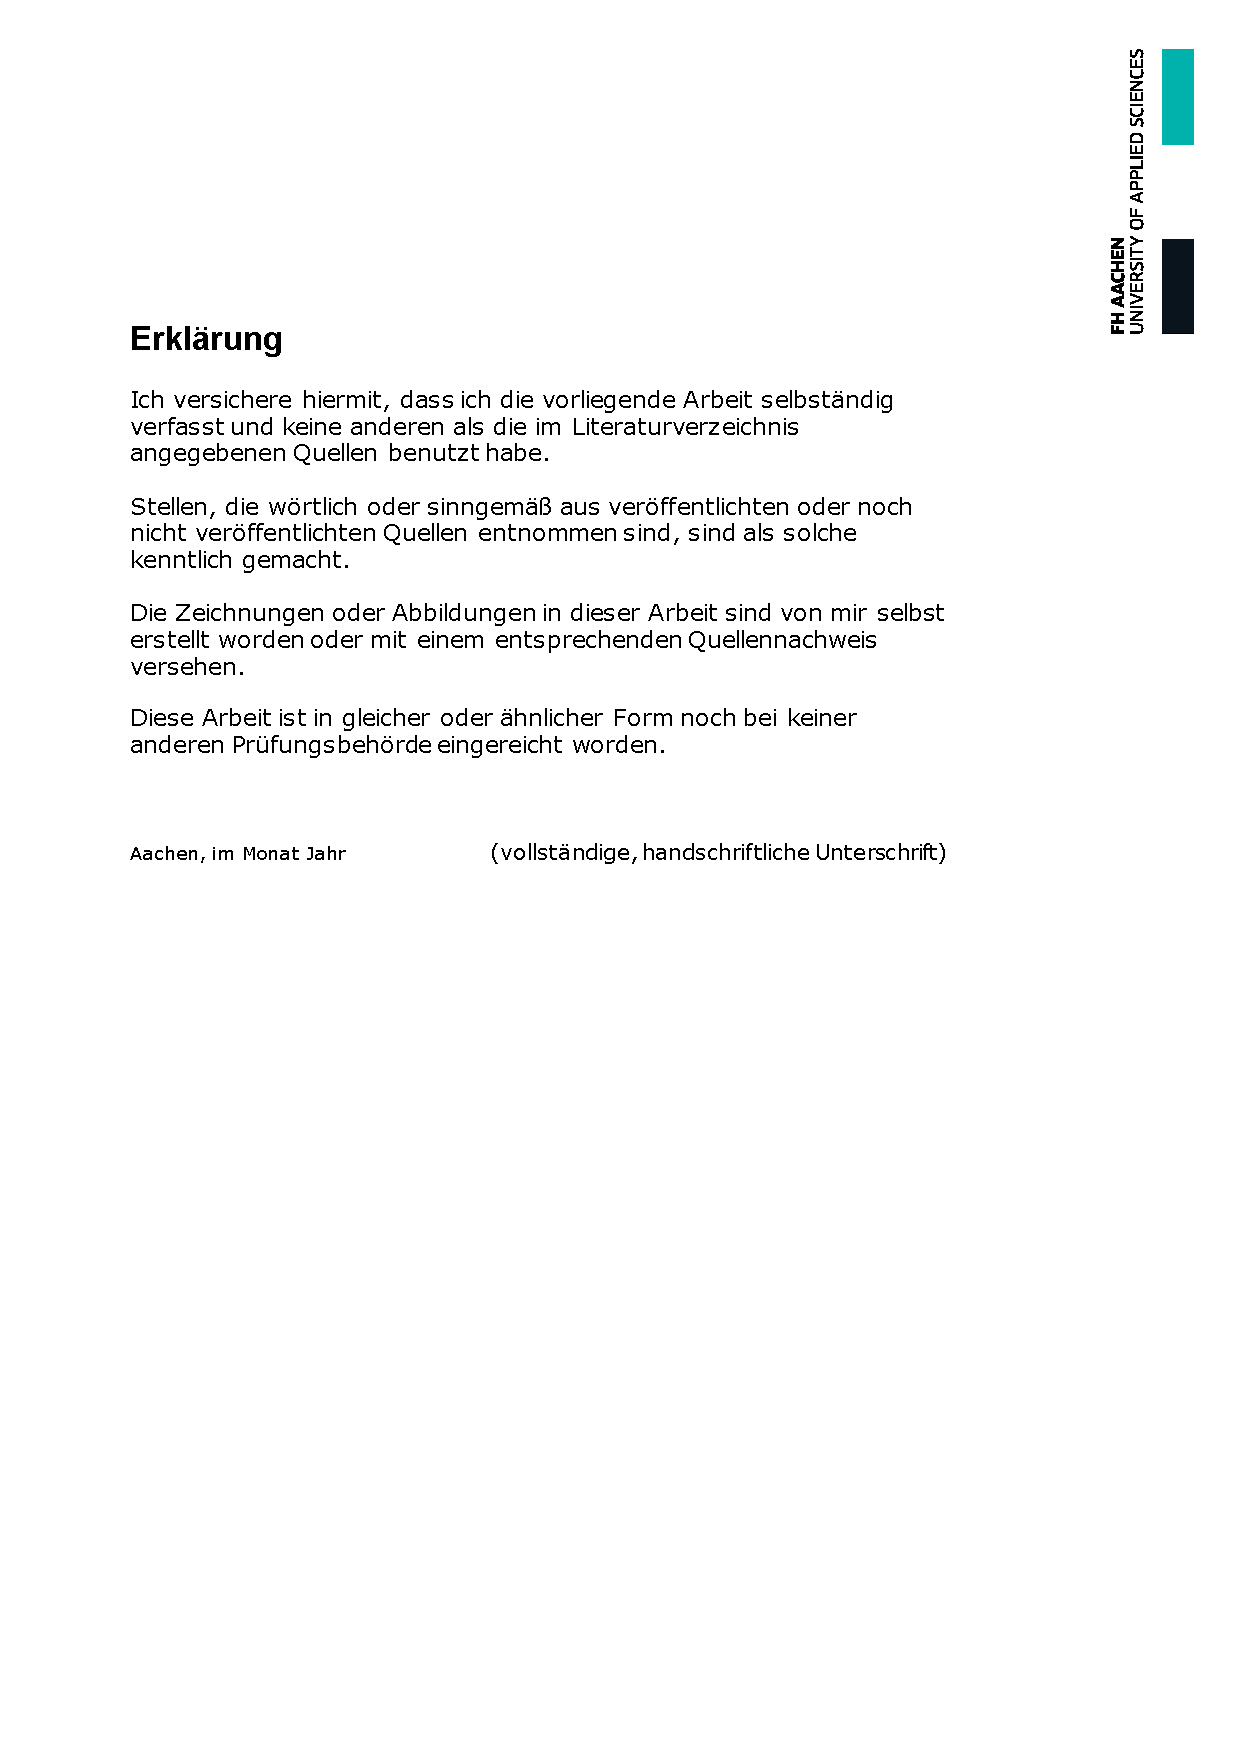
\includepdf[pages={1}]{./external/Bachelorarbeit_Erklaerung.pdf}
    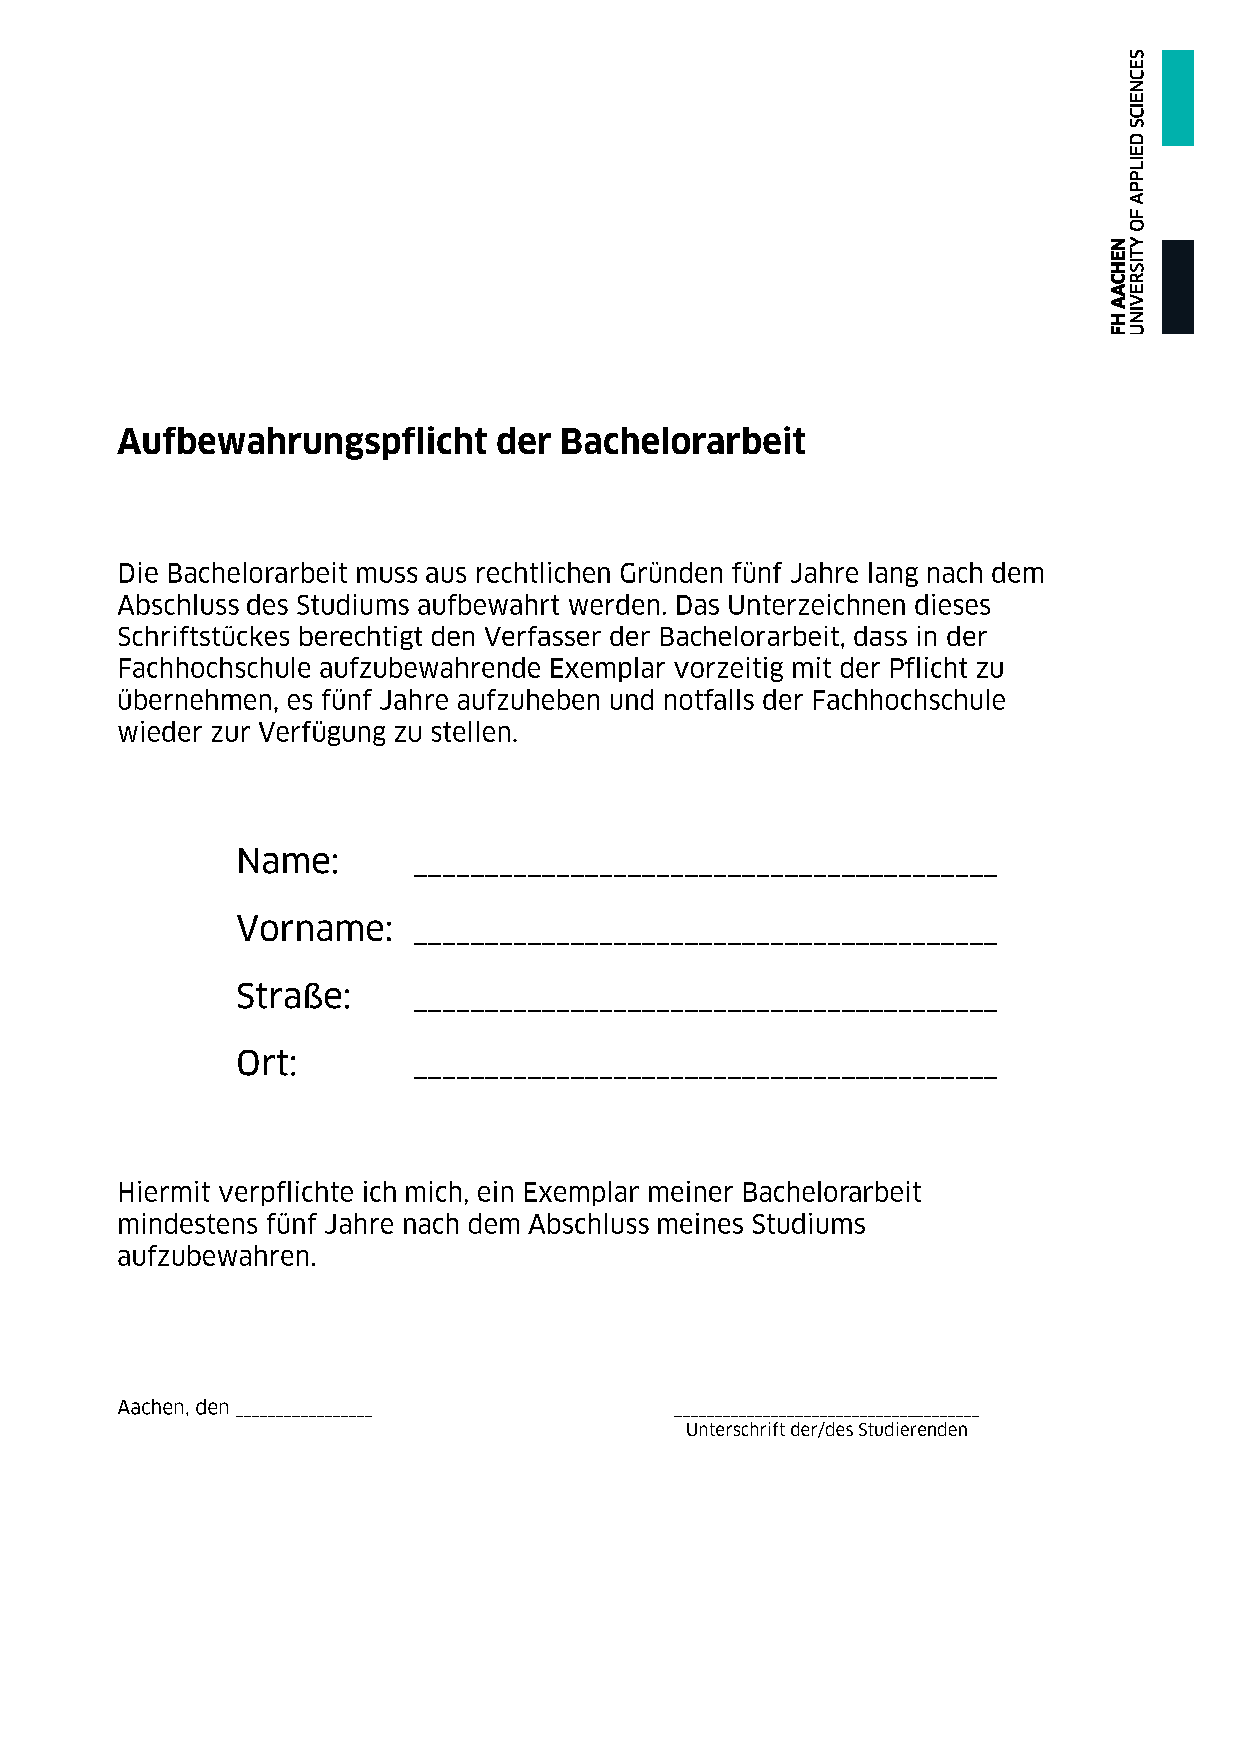
\includepdf[pages={1}]{./external/Bachelorarbeit_Aufbewahrungspflicht.pdf}



    \pagenumbering{gobble} %no page numbering
    \setcounter{page}{1} %counter for page numbering is set to 1
    \pagenumbering{Roman} % page numbering is done with capital roman signs (I, II, III...)
    \clearpage
\setlength{\parskip}{0.5em}

\markboth{\textbf{Abstract}}{\textbf{Abstract}}\label{abstract}

\textbf{Abstract}

\textit{Kann ein KI-gestützter Tutor den Einstieg ins Programmieren erleichtern?}


Die vorliegende Bachelorarbeit untersucht, inwiefern die Integration eines KI-gestützten Chat-Tutors und einer adaptiven Drill-Auswahl die Lernerfahrung beim Erwerb von Python-Grundlagen verbessert. Hierzu wurde ein webbasiertes Lernsystem entwickelt, das Einsteigende schrittweise durch die Implementierung eines vollständigen BMI-Rechner-Programms führt und dabei KI-basierte Assistenz über die OpenAI-API integriert. Als theoretischer Rahmen dient das 4C/ID-Modell (Four-Component Instructional Design) nach van Merriënboer, wobei der Fokus auf den Komponenten Learning Tasks und Part-task Practice liegt.

Eine kontrollierte empirische Studie mit 18 Teilnehmenden im Between-Subjects-Design untersuchte, ob KI-gestützte Komponenten zu günstigeren Lernindikatoren führen. Die Kontrollgruppe (Gruppe~A) arbeitete ohne KI-Funktionen, während die Experimentalgruppe (Gruppe~B) Zugang zu KI-gestützter Aufgabenauswahl und einem KI-Chat-Tutor erhielt. Die Datenerhebung umfasste System-Logs, NASA-TLX-Fragebögen, Usability-Skalen sowie KI-spezifische Evaluationsitems.

Die Ergebnisse zeigen keine signifikanten Unterschiede in objektiven Leistungsindikatoren wie Fehlerrate oder Abschlussquote. Auf subjektiver Ebene wies Gruppe~B konsistent günstigere Werte auf: geringere Frustration im NASA-TLX, höhere hedonische Qualität im UEQ-S sowie einen besseren Net Promoter Score. Eine qualitative Analyse der Chat-Verläufe identifizierte sowohl produktive Nutzungsmuster als auch systemseitige Schwachstellen, aus denen konkrete Verbesserungsmaßnahmen abgeleitet werden.

\setlength{\parskip}{0pt}
\clearpage


    % Danksagung (vor dem Inhaltsverzeichnis)
    \markright{\textbf{Danksagung}}
    \markleft{\textbf{Danksagung}}
    \clearpage
\chapter*{\textbf{Danksagung}}\label{acknowledgements}

Die vorliegende Bachelorarbeit bildet den vorerst letzten Meilenstein meines Informatik Studiums und schließt eine prägende Lebensphase ab. Auch wenn dieser Abschluss einen vorläufigen Endpunkt setzt, blicke ich mit Neugier auf zukünftige akademische Herausforderungen, die folgen mögen. Die Erstellung dieser Arbeit wäre ohne die fachliche und persönliche Unterstützung vieler Wegbegleiter nicht möglich gewesen.

Mein besonderer Dank gilt meinem Betreuer, Herrn Prof.~Dr.~rer.~pol. Christian Drumm, für die Ermöglichung dieses spannenden Themas sowie für die wertvollen Impulse und die stets konstruktive fachliche Begleitung während des gesamten Prozesses.

Des Weiteren möchte ich meinen Freunden und Kommilitonen für den steten Austausch und die gegenseitige Motivation danken. Ein herzlicher Dank geht dabei insbesondere an meinen Mitbewohner für sein gewissenhaftes Korrekturlesen und das wertvolle Feedback, welches maßgeblich zur Qualität dieser Arbeit beigetragen hat.

Ein ganz persönlicher Dank gebührt meiner Familie und meiner Partnerin. Danke, dass ihr mich nicht nur in den letzten Monaten, sondern über die vergangenen Jahre hinweg unermüdlich unterstützt habt. Euer Rückhalt und eure Geduld waren die Basis, auf der ich dieses Studium erfolgreich absolvieren konnte.

\vspace{2cm}

\noindent
Erkelenz, den \today

\vspace{1.5cm}

\noindent
Kacper Cömlek

%\addtocontents{toc}{\vspace{0.8cm}}


    % Table of contents is generated:
    \makeatletter
    \renewcommand*{\@dotsep}{1} % set gap between dots
    \makeatother
    \tableofcontents

    % First chapter starts on uneven number
    \cleardoublepage
    \setstretch{1.25}
    \pagenumbering{arabic} %page numbering is done with arabic numbers

    % Kapitelstruktur der Bachelorarbeit
    \clearpage

\chapter{\textbf{Einleitung}}\label{ch:einleitung}

Dieses Kapitel beschreibt die Ausgangslage und Motivation der Arbeit, formuliert die Forschungsfrage sowie die zentrale Hypothese und erläutert den Aufbau der vorliegenden Ausarbeitung.

\section{Problemstellung}\label{sec:problemstellung}

Python gehört zu den meistgenutzten Programmiersprachen weltweit und ist in Bereichen wie Datenanalyse, Automatisierung und Künstlicher Intelligenz zur Standardsprache geworden~\cite{stackoverflow2024}. Die Nachfrage nach Personen mit grundlegenden Programmierkenntnissen wächst branchenübergreifend und immer mehr Bildungseinrichtungen reagieren darauf mit eigenen Einführungskursen in Python. Gleichzeitig zeigt die Forschung zur Programmierausbildung konsistent, dass gerade der Einstieg mit hohen Abbruchquoten und ausgeprägten Frustrationserlebnissen verbunden ist~\cite{bennedsen2007}. Die binäre Fehlerkultur der Programmierung, in der bereits ein fehlendes Klammerpaar zum vollständigen Programmabbruch führt, stellt viele Einsteigende vor eine Hürde, die sie schon vor dem Verständnis grundlegender Konzepte wie Variablen, Schleifen oder Listenstrukturen kapitulieren lässt~\cite{jenkins2002}. Dijkstra beschrieb dieses Phänomen treffend als \textit{Radical Novelty}: Programmieren unterscheidet sich in seiner Fehlerintoleranz fundamental von anderen Lerngegenständen, da selbst minimale Tippfehler das gesamte Programm zum Absturz bringen.

Ein zentrales Problem bestehender Lernangebote ist das Fehlen unmittelbarer, individualisierter Unterstützung im Fehlerfall. Klassische Lehrformate wie Lehrbücher oder Vorlesungen können auf individuelle Fehler nicht in Echtzeit eingehen. Online-Lernplattformen bieten zwar interaktive Aufgaben, arbeiten aber mit statischem, vordefiniertem Feedback, das nicht auf den spezifischen Code einer lernenden Person eingeht. MOOCs im Hochschulbereich leiden unter demselben Problem in noch stärkerem Ausmaß: Bei Tausenden eingeschriebenen Lernenden ist individuelle Betreuung strukturell nicht möglich. Wenn Einsteigende in einer Aufgabe feststecken und keine Orientierung finden, beschreibt Jenkins~\cite{jenkins2002} das entstehende Erleben als \textit{Learned Helplessness}, also das Gefühl der Hilflosigkeit, das schnell in Frustration und Kursabbruch umschlägt.

Gleichzeitig haben sich die technischen Möglichkeiten zur KI-gestützten Lernunterstützung in den letzten Jahren fundamental verändert. Große Sprachmodelle wie GPT-4 sind in der Lage, Programmiercode zu verstehen, Fehlermeldungen zu interpretieren und didaktisch sinnvolles Feedback auf natürlichsprachliche Anfragen zu geben~\cite{kasneci2023}. Während frühere Tutorsysteme aufwendig von Hand zu kuratieren waren, ermöglicht die OpenAI-API heute die Integration dieser Fähigkeiten in webbasierte Lernanwendungen mit vertretbarem Entwicklungsaufwand. Die entscheidende offene Frage ist dabei nicht mehr, ob solche Systeme technisch realisierbar sind, sondern ob sie tatsächlich besser lernen lassen als Systeme ohne KI-Unterstützung und welche didaktischen Designentscheidungen dafür ausschlaggebend sind.


\section{Zielsetzung und Forschungsfrage}\label{sec:zielsetzung}

Diese Arbeit verfolgt zwei eng miteinander verbundene Ziele. Erstens wird ein webbasiertes Lernsystem für Python-Grundlagen entwickelt und implementiert, das auf dem didaktischen Rahmen des \textit{Four-Component Instructional Design} (4C/ID-Modell) nach van Merriënboer basiert. Der Schwerpunkt liegt auf zwei Komponenten des Modells: authentischen \textit{Learning Tasks} in Form eines geführten Programmierkurses, der Lernende schrittweise durch ein vollständiges BMI-Rechner-Programm führt, sowie adaptiver \textit{Part-task Practice} durch KI-gestützte Drill Tasks\footnote{Unter \textit{Drill Tasks} werden kurze, isolierte Wiederholungsaufgaben verstanden, die gezielt einzelne Teilfähigkeiten trainieren, z. B. das Schreiben einer einfachen \texttt{print()}-Anweisung oder das Konkatenieren von Strings.}. Als KI-Komponenten kommen ein kontextgebundener Chat-Tutor mit progressivem Hint-System und ein auf der OpenAI-API (Modell \texttt{gpt-4o-mini}) basierender Algorithmus zur Drill-Auswahl zum Einsatz.

Zweitens wird dieses System in einer kontrollierten empirischen Studie mit 18 Teilnehmenden erprobt. In einem \textit{Between-Subjects-Design} (d.\,h. jede Person gehört genau einer Gruppe an und sieht nur eine der beiden Varianten) bearbeiten zwei Gruppen denselben Kurs: Die Kontrollgruppe (Gruppe~A) nutzt das System ohne KI-Funktionen und die Experimentalgruppe (Gruppe~B) mit KI-Tutor und adaptiver Drillauswahl.
Um zu verstehen, ob und wie sich diese beiden Lernumgebungen unterscheiden, werden Verhaltens- und Erlebensdaten aus mehreren Perspektiven erfasst: objektive Leistungsdaten aus den System-Logs, die subjektiv wahrgenommene kog\-nitive Belastung, die Gebrauchstauglichkeit (Usability) sowie KI-spezifische Evaluationsaspekte.

Die dabei leitende Forschungsfrage lautet:

\begin{quote}
\textit{Inwiefern verbessert die Integration einer KI-gestützten Drill-Auswahl und eines KI-Tutors die lernbezogenen Indikatoren und die wahrgenommene Lernunterstützung beim Erlernen von Python-Grundlagen im Vergleich zu einem Basis-System ohne diese Komponenten?}
\end{quote}

Aus dieser Frage wird eine gerichtete Haupthypothese abgeleitet: Lernende in der Experimentalgruppe (Gruppe~B) weisen im Vergleich zur Kontrollgruppe (Gruppe~A) günstigere lernbezogene Indikatoren in den Systemlogs sowie eine höhere subjektive Zufriedenheit mit der Lernunterstütz\-ung auf. Die Operationalisierung dieser Hypothese und das vollständige Studiendesign werden in Kapitel~\ref{ch:studie} beschrieben.

\clearpage

\section{Aufbau der Arbeit}\label{sec:aufbau}

Die vorliegende Arbeit gliedert sich in acht Kapitel:

\textbf{Kapitel~\ref{ch:grundlagen}} legt die theoretischen Grundlagen dar. Es werden zunächst die Herausforderungen der Programmierausbildung für Einsteigende beleuchtet, anschließend das 4C/ID-Modell als didaktischer Rahmen vorgestellt und schließlich der Einsatz von KI im Bildungskontext diskutiert. Das Kapitel schließt mit einer Abgrenzung zu verwandten Arbeiten.

\textbf{Kapitel~\ref{ch:konzeption}} beschreibt die Konzeption des Lernsystems. Ausgehend von einer Anforderungsanalyse wird das didaktische Konzept entwickelt und die Systemarchitektur einschließlich der KI-Anbindung dargestellt.

\textbf{Kapitel~\ref{ch:implementierung}} dokumentiert die technische Umsetzung des Prototyps. Es werden die Technologieauswahl begründet, die Kernkomponenten beschrieben und auf Herausforderungen während der Entwicklung eingegangen.

\textbf{Kapitel~\ref{ch:studie}} erläutert das Design der empirischen Studie. Hier werden Forschungsdesign, Hypothesen, Stichprobe, Studienablauf sowie die erhobenen Daten und Messinstrumente beschrieben.

\textbf{Kapitel~\ref{ch:ergebnisse}} präsentiert die Ergebnisse der Studie in deskriptiver und vergleichender Form, ergänzt durch qualitative Erkenntnisse aus den Freitextantworten.

\textbf{Kapitel~\ref{ch:diskussion}} interpretiert die Ergebnisse, ordnet sie in den Forschungsstand ein und beleuchtet auf Basis einer qualitativen Sichtung der Chat-Verläufe konkrete Stärken und Schwachstellen des KI-Tutors. Abschließend werden Limitationen benannt und Implikationen für Forschung und Praxis abgeleitet.

\textbf{Kapitel~\ref{ch:fazit}} fasst die zentralen Erkenntnisse zusammen und gibt einen Ausblick auf weiterführende Forschung und Systementwicklung.


Sämtliche anonymisierten Studiendaten, wie Chat-Verläufe, Aufgaben-Log-Daten und Fragebogenantworten, sind zusammen mit dem Quellcode des Systems im öffentlichen GitHub-Pro\-jekt archiviert und für weiterführende Auswertungen verfügbar (vgl.\ \hyperref[appendix:daten]{Anhang~D}).


\addtocontents{toc}{\vspace{0.8cm}}
    % Kapitel 1: Einleitung
    \chapter{\textbf{Theoretische Grundlagen}}\label{ch:grundlagen}

Dieses Kapitel bildet die theoretischen Grundlagen für die Konzeption und Evaluation des in dieser Arbeit entwickelten Lernsystems. Zunächst werden die Herausforderungen der Programmierausbildung für Einsteigende dargestellt. Darauf aufbauend wird das 4C/ID-Modell als didaktischer Rahmen eingeführt, einschließlich seiner lerntheoretischen Grundlagen. Anschließend wird der Einsatz von KI im Bildungskontext beleuchtet. Das Kapitel schließt mit einer Einordnung verwandter Arbeiten ab.


\section{Programmierausbildung für Einsteigende}\label{sec:programmierausbildung}

Das Erlernen von Programmierung gilt als anspruchsvolle kognitive Tätigkeit, die Einsteigende vor spezifische Hürden stellt. Im Folgenden werden diese Herausforderungen dargestellt, bestehende Lösungsansätze eingeordnet und die Rolle von Übung und Feedback für den Kompetenzerwerb beleuchtet.

\subsection{Herausforderungen beim Programmierenlernen}\label{subsec:herausforderungen}

Das Erlernen von Programmierung stellt Einsteigende vor erhebliche Herausforderungen. Tomaschitz beschreibt den Programmierprozess als \enquote{vielschichtig und komplex} und betont, dass analytische, mathematische und logische Fertigkeiten erforderlich sind, \enquote{um Spezifikationen zu lesen, in Algorithmen umzuwandeln und syntaktisch korrekten Code zu schreiben}~\cite{tomaschitz2020}. Dabei müssen drei kognitive Anforderungen simultan bewältigt werden.
Erstens erfordert das \textit{Problemverständnis} die Fähigkeit, die Anforderungen einer Programmieraufgabe zu erfassen und in eine mentale Repräsentation zu überführen. Zweitens ist \textit{algorithmisches Denken} notwendig, um die Schritte zur Lösung des Problems zu planen und in eine logische Abfolge zu bringen. Drittens muss die \textit{Codeproduktion} erfolgen, also die Umsetzung der geplanten Lösung in syntaktisch korrekten Code. Diese Gleichzeitigkeit führt insbesondere bei Einsteigenden zu kognitiver Überlastung, da keine der drei Anforderungen isoliert bewältigt werden kann.

Programmieren wird als hierarchische Kompetenz charakterisiert: \enquote{Programming is not a single skill. It is also not a simple set of skills; the skills form a hierarchy}~\cite{jenkins2002}. Diese Hierarchie reicht von der Syntax über die Semantik bis hin zur Programmstruktur und zum Programmierstil. Einsteigende müssen diese Ebenen nacheinander aufbauen und verbleiben häufig auf der syntaktischen Ebene, ohne ein tieferes Verständnis zu entwickeln. Als zentrale Überforderungsquelle wird dabei die Gleichzeitigkeit zweier Lernprozesse beschrieben. Einerseits erfordert \textit{Surface Learning} das Auswendiglernen syntaktischer Regeln, andererseits verlangt \textit{Deep Learning} das Durchdringen der zugrundeliegenden Logik~\cite{jenkins2002}.

Ein besonderes Merkmal der Programmierung ist ihre Fehlerintoleranz. Dijkstra beschreibt Programmierung als \enquote{precision intensive -- the smallest possible perturbation of one single bit can render a program totally worthless}~\cite{jenkins2002}.

In kaum einem anderen Fach führt ein minimaler Fehler, wie etwa ein fehlender Doppelpunkt oder eine falsche Einrückung in Python, zum vollständigen Scheitern des Programms. Diese von Dijkstra als \textit{Radical Novelty} bezeichnete Andersartigkeit des Programmierens unterscheidet es von anderen Lerndisziplinen und erklärt die hohe Frustration unter Einsteigenden.


Die empirische Forschung bestätigt diese Schwierigkeiten auf breiter Basis. Qian und Lehman identifizieren in ihrer Literaturübersicht zahlreiche \textit{Misconceptions}\footnote{Mit \textit{Misconceptions} sind typische Fehlvorstellungen gemeint, die Lernende bei grundlegenden Programmierkonzepten entwickeln.} bei Programmiereinsteigenden, insbesondere bei Variablenzuweisungen, die häufig als mathematische Gleichungen statt als Speicheroperationen interpretiert werden~\cite{qian2017}. 

Auch das mentale Modell, das als \textit{Notional Machine}\footnote{Die \textit{Notional Machine} beschreibt ein vereinfachtes mentales Modell darüber, wie ein Programm intern ausgeführt wird (z.\,B. Zustandsänderungen von Variablen Schritt für Schritt).} bezeichnet wird, bereitet nachweislich Schwierigkeiten. 
Lernende müssen dabei ein Verständnis dafür aufbauen, wie der Computer Anweisungen ausführt, um Programmabläufe nachvollziehen zu können~\cite{sorva2013}. Bennedsen und Caspersen berichten von durchschnittlichen Durchfallquoten von 33\,\% in einführenden Programmierkursen weltweit~\cite{bennedsen2007}.

Diese Herausforderungen werden durch das typische Lehrsetting verschärft. Einführungskurse werden als \enquote{high-speed train with no brakes} beschrieben, in denen Lernende, die einmal den Anschluss verlieren, in einen Zustand der \textit{Learned Helplessness} geraten~\cite{jenkins2002}. Das feste Kurstempo lässt wenig Raum für individuelles Lerntempo, welches ein zentrales Argument für adaptive und technologiegestützte Lernsysteme ist.

Die vorliegende Arbeit fokussiert sich auf Python als Programmiersprache. Python eignet sich als Einstiegssprache, da die Syntax sich an natürlicher Sprache orientiert, auf geschweifte Klammern und Semikolons verzichtet und durch dynamische Typisierung die initiale Hürde senkt~\cite{luxton2018}. Gleichzeitig ist Python die weltweit meistgenutzte Programmiersprache~\cite{tiobe2025} und besitzt hohe praktische Relevanz für Datenanalyse, Automatisierung und für einen Einsatz außerhalb der professionellen Softwareentwicklung.


\subsection{Bestehende Ansätze und deren Grenzen}\label{subsec:bestehende-ansaetze}

Für das Erlernen von Programmierung existiert eine Vielzahl von Ansätzen und Plattformen. Online-Plattformen wie Codecademy oder freeCodeCamp bieten interaktive Kurse mit eingebetteten Programmierübungen und haben die Zugänglichkeit der Programmierausbildung erheblich verbessert. MOOCs (\textit{Massive Open Online Courses}) ermöglichen den Zugang zu Hochschulkursen für ein breites Publikum. Visuelle Programmierumgebungen wie Scratch adressieren den niedrigschwelligen Einstieg, beschränken sich jedoch auf blockbasierte Programmierung und bereiten nicht unmittelbar auf textbasierte Sprachen vor~\cite{luxton2018}.

Aus Sicht des in dieser Arbeit gewählten didaktischen Rahmens weisen diese Ansätze jedoch gemeinsame Limitationen auf. Erstens bieten die meisten Plattformen wenig Individualisierung: Alle Lernenden durchlaufen dieselbe Aufgabensequenz unabhängig von ihrem Lernstand oder ihren spezifischen Schwierigkeiten. Zweitens beschränkt sich das Feedback häufig auf eine binäre Rückmeldung (richtig/falsch), ohne detaillierte Erklärungen zu liefern, warum eine Lösung fehlerhaft ist. Drittens ist die Aufgabenreihenfolge bei vielen Plattformen didaktisch nur schwach begründet, da sie meist einer thematischen Abfolge entspricht und nicht auf einem lerntheoretisch fundierten Modell basiert. Diese Limitationen machen eine Lücke deutlich, die die vorliegende Arbeit schließt: die Kombination eines evidenzbasierten didaktischen Modells mit KI-gestützter Individualisierung von Übungsaufgaben und Feedback.


\subsection{Bedeutung von Übung und Feedback}\label{subsec:uebung-feedback}

Nicht die bloße Übungszeit, sondern die Qualität des Übens und die Unmittelbarkeit des Feedbacks entscheiden über den Lernerfolg. Ericsson, Krampe und Tesch-Römer prägen den Begriff der \textit{Deliberate Practice}\footnote{\textit{Deliberate Practice} bezeichnet gezieltes, wiederholtes Üben mit klaren Lernzielen und zeitnahem, informativem Feedback.}: Gezielte, wiederholte Übung mit informativem Feedback ist wirksamer als passives Aufnehmen oder unstrukturiertes Üben~\cite{ericsson1993}. Entscheidend ist dabei nicht die Anzahl der Wiederholungen allein, sondern die Qualität der Übung, diese muss auf spezifische Schwächen ausgerichtet sein und korrigierendes Feedback bereitstellen.

Hattie und Timperley identifizieren in ihrer Meta-Analyse Feedback als einen der einflussreichsten Faktoren für den Lernerfolg~\cite{hattie2007}. Besonders wirksam ist das sogenannte \textit{Process Feedback}\footnote{\textit{Process Feedback} bezieht sich auf den Lösungsprozess (z.\,B. Strategie und Vorgehen) und nicht nur auf das Ergebnis (richtig/falsch).}, das nicht nur die Korrektheit bewertet, sondern Hinweise auf den Lösungsweg gibt und zur Selbstregulation anregt. Während unmittelbares Feedback insbesondere auf der Aufgabenebene (\textit{Task Level}) vorteilhaft ist, ermöglicht die zeitnahe Verfügbarkeit in automatisierten Systemen eine kontinuierliche Begleitung des Lernprozesses, die durch Lehrkräfte in dieser Frequenz kaum zu leisten ist~\cite{hattie2007}.

Für die Programmierausbildung bedeutet dies, dass Übungsaufgaben nicht primär als Prüfungs\-instrument dienen sollten. Stattdessen erfüllen sie die Funktion eines \textit{formativen Assessments} und unterstützen Lernende dabei, ihren aktuellen Wissensstand einzuschätzen.

Tomaschitz bestätigt dies empirisch: Der Einsatz eines Überprüfungstools, das visuelles Feedback über den Code lieferte, steigerte die Leistung der Studierenden und führte zu erhöhtem Lernerfolg~\cite{tomaschitz2020}. KI-basierte Systeme eröffnen hier neue Möglichkeiten, da sie über vordefinierte Regeln hinaus kontextbezogene, individuelle Rückmeldungen generieren und damit die Funktion eines persönlichen Tutors annähern können.


%% ============================================================================
%% ABSCHNITT 2.2
%% ============================================================================

\section{Didaktischer Rahmen: Das 4C/ID-Modell}\label{sec:4cid}

Aufbauend auf den in Abschnitt~\ref{sec:programmierausbildung} dargestellten Herausforderungen wird nun der didaktische Rahmen eingeführt, der das Lernsystem dieser Arbeit strukturiert. Zunächst werden die lerntheoretischen Grundlagen gelegt, bevor das 4C/ID-Modell im Detail vorgestellt wird.

\subsection{Cognitive Load Theory}\label{subsec:clt}\label{subsec:lerntheorie}

Die \textit{Cognitive Load Theory} nach Sweller, im Folgenden als CLT bezeichnet, bildet das theoretische Fundament des 4C/ID-Modells~\cite{sweller1988}. Die CLT geht von der Annahme aus, dass das menschliche Arbeitsgedächtnis eine begrenzte Kapazität besitzt und gleichzeitig nur eine begrenzte Anzahl von Informationselementen verarbeiten kann. Wird diese Kapazität überschritten, ist effektives Lernen nicht möglich. Sweller, van Merriënboer und Paas unterscheiden drei Arten kognitiver Belastung~\cite{sweller1998}:

\begin{itemize}
    \item \textbf{Intrinsic Load} entsteht durch die enthaltene Komplexität des Lernstoffs. Er wird durch die Anzahl der untereinander interagierenden Elemente bestimmt und kann durch geschickte Anordnung gesteuert werden. Dies lässt sich beispielsweise erreichen, indem einfache Konzepte vor komplexeren eingeführt werden.
    \item \textbf{Extraneous Load} entsteht aus der Gestaltung der Lernumgebung selbst und trägt nicht zum Lernen an sich bei. Er sollte minimiert werden, etwa durch klare Instruktionsdesigns und bedarfsgerechte Hilfestellungen.
    \item \textbf{Germane Load} bezeichnet die produktive kognitive Belastung, die für den Aufbau und die Automatisierung mentaler Schemata genutzt wird. Ein effektives Instruktionsdesign zielt darauf ab, kognitive Ressourcen für diesen Lernprozess optimal zu nutzen.
\end{itemize}

Für die Programmierausbildung ist die CLT besonders relevant, da Einsteigende typischerweise einem hohen Intrinsic Load ausgesetzt sind, wie Abschnitt~\ref{subsec:herausforderungen} zeigt. Das 4C/ID-Modell adressiert alle drei Load-Typen systematisch. Aufgabenklassen mit steigender Komplexität steuern den Intrinsic Load, unterstützende Strukturen wie \textit{Scaffolding}\footnote{\textit{Scaffolding} bezeichnet unterstützende Hilfen, die Lernenden anfangs Orientierung geben und mit zunehmender Kompetenz schrittweise reduziert werden.} und klare Instruktionen reduzieren den Extraneous Load und gezielte Übungen fördern die Schemaautomatisierung und damit den Germane Load.

\clearpage
\subsection{Selbstreguliertes Lernen}\label{subsec:srl}

Da das in dieser Arbeit entwickelte Lernsystem vollständig ohne Lehrkraft genutzt wird, ist das Konzept des \textit{selbstregulierten Lernens} nach Zimmerman von zentraler Bedeutung \cite{zimmerman2002, panadero2017, winne2005}. 

Selbstreguliertes Lernen, im Folgenden als SRL bezeichnet, beschreibt den Prozess, in dem Lernende ihre eigenen Lernaktivitäten planen, überwachen und bewerten.

In digitalen, selbstgesteuerten Lernumgebungen müssen Lernende diese metakognitiven Fähig\-keiten eigenständig einsetzen, was speziell bei Einsteigenden zu Überforderung führen kann \cite{winne2005}.
Ohne externe Regulation besteht das Risiko, dass Lernende schwierige Inhalte überspringen oder ihren Lernstand falsch einschätzen. Dazu zählen auch systematische Fehlurteile und Illusionen beim selbstregulierten Lernen \cite{bjork2013}.
In KI-gestützten Umgebungen besteht zudem die Gefahr, dass Lernende den KI-Chatbot vorrangig als unmittelbares Lösungs\-werkzeug nutzen, anstatt ihn als lernförderliche Unterstützung einzubinden \cite{kazemitabaar2023}.
Digitale Lernumgebungen müssen daher Mechanismen der externen Regulation bereitstellen. Dazu gehören etwa verpflichtende Übungsphasen, gestufte Hilfestellungen oder Fortschrittsanzeigen, um SRL auch bei Einsteigenden zu ermöglichen \cite{azevedo2005}. Wie das vorliegende System diesen Anforderungen konkret begegnet, wird in Kapitel~\ref{ch:konzeption} beschrieben.


\subsection{Das 4C/ID-Modell im Überblick}\label{subsec:4cid-ueberblick}

Das \textit{Four-Component Instructional Design}, kurz 4C/ID, wurde von van Merriënboer entwickelt und bietet einen systematischen Ansatz zur Gestaltung von Lernumgebungen für komplexe kognitive Fähigkeiten~\cite{vanmerrienboer2018, vanmerrienboer2003}. Das Modell basiert explizit auf der CLT und strukturiert den Lernprozess in vier miteinander verknüpfte Komponenten:

\begin{enumerate}
    \item \textbf{Learning Tasks:} Authentische, ganzheitliche Aufgaben in realitätsnahen Kontexten. Sie sind in Aufgabenklassen mit steigender Komplexität organisiert.
    \item \textbf{Supportive Information:} Konzeptuelles Wissen und theoretische Hintergründe, die den Aufbau mentaler Modelle fördern und vor oder während der Aufgabenbearbeitung bereitgestellt werden.
    \item \textbf{Just-in-time Information:} Prozedurale Anleitungen und Handlungsanweisungen, die genau dann bereitgestellt werden, wenn sie benötigt werden.
    \item \textbf{Part-task Practice:} Isoliertes Üben von Teilfertigkeiten zur Automatisierung wiederkehrender Prozesse.
\end{enumerate}

Ausgehend von den dargestellten Herausforderungen beim Programmierenlernen und der Cog\-nitive Load Theory wird das 4C/ID-Modell in dieser Arbeit als didaktischer Rahmen gewählt \cite{vanmerrienboer2018, vanmerrienboer2003}. 

Erstens enthält das Modell mit der Part-task Practice einen expliziten Mechanismus für isoliertes Üben, der sich gut für die technologische Umsetzung und Automatisierung eignet \cite{vanmerrienboer2018}. 
Zweitens strukturiert 4C/ID den Lernstoff in Aufgabenklassen mit steigender Komplexität und ermöglicht dadurch eine nachvollziehbare Progression \cite{vanmerrienboer2018, vanmerrienboer2003}. 
Drittens ist das Modell evidenzbasiert und in der Hochschuldidaktik etabliert \cite{frerejean2019}. 
Viertens adressiert 4C/ID durch seine Fundierung in der CLT das Risiko kognitiver Überlastung, das insbesondere bei Programmiereinsteigenden relevant ist \cite{sweller1998, vanmerrienboer2018}.
Die konkrete Umsetzung dieser Prinzipien im vorliegenden System wird in Kapitel~\ref{ch:konzeption} beschrieben.


\subsection{Die vier Komponenten im Detail}\label{subsec:4cid-komponenten}

Das Modell gliedert sich in vier aufeinander abgestimmte Komponenten, die im Folgenden einzeln dargestellt werden.

\paragraph{Learning Tasks: Lernaufgaben}

Lernaufgaben bilden das Kernstück des 4C/ID-Modells. Sie basieren auf authentischen, ganzheitlichen Aufgaben, die in der Literatur als \textit{Whole Tasks} beschrieben werden und Wissen, Fertigkeiten sowie Haltungen integrieren, die für die Bewältigung von Aufgaben im zukünftigen Beruf oder Alltag benötigt werden~\cite{niegemann2020}. Im Gegensatz zu isolierten Teilübungen konfrontieren sie die Lernenden mit der gesamten Komplexität einer Problemstellung.

Lernaufgaben werden in \textit{Aufgabenklassen} organisiert, die eine steigende Komplexität abbilden. Innerhalb einer Klasse erhalten Lernende zunächst Unterstützung, die als \textit{Scaffolding} beschrieben wird. Mit zunehmender Kompetenz wird diese Unterstützung schrittweise zurückgenommen, was als \textit{Fading}\footnote{\textit{Fading} beschreibt den schrittweisen Abbau anfänglicher Unterstützung, damit Lernende Aufgaben zunehmend selbstständig lösen.} bezeichnet wird. Niegemann und Weinberger betonen, dass Lernen durch Entdecken nur dann effektiv ist, wenn die Lernaufgaben untereinander \enquote{eine gewisse Variation aufweisen}~\cite{niegemann2020}.

\paragraph{Supportive Information: Unterstützende Informationen}

Unterstützende Informationen helfen Lernenden bei den nicht-routinisierbaren Aspekten der Lernaufgaben, die Problemlösen und Entscheidungen erfordern. Van Merriënboer und Kirschner beschreiben sie als das konzeptuelle Wissen, das den Aufbau \textit{mentaler Modelle} fördert~\cite{vanmerrienboer2018}. Typische Formen sind theoretische Erklärungen, Analogien sowie \textit{Worked Examples}, also ausgearbeitete Lösungsbeispiele.

Die unterstützenden Informationen sind nicht an einzelne Aufgaben gebunden, sondern an die jeweilige Aufgabenklasse: Sie werden idealerweise vor Beginn einer neuen Klasse bereitgestellt und können während der Bearbeitung abgerufen werden~\cite{niegemann2020}. Bei steigender Kompetenz werden sie schrittweise reduziert.

\paragraph{Just-in-time Information: Prozedurale Information}

Im Gegensatz zur unterstützenden Information wird die prozedurale Information genau dann bereitgestellt, wenn sie benötigt wird. Sie umfasst konkrete Handlungsanweisungen, die als \textit{How-to-Instruktionen} bezeichnet werden und für die Ausführung routinisierbarer Aspekte der Aufgabe erforderlich sind~\cite{niegemann2020}.

Niegemann und Weinberger heben einen Vorteil menschlicher Lehrkräfte gegenüber statischen Anleitungen hervor: \enquote{Der Vorteil eines Lehrers gegenüber einer Benutzeranleitung besteht darin, dass ein Lehrer gewissermaßen über die Schulter schauen kann und Anweisungen und korrektives Feedback genau dann geben kann, wenn es benötigt wird}~\cite{niegemann2020}. Für digitale Lernumgebungen liegt nahe, dass ein KI-Chatbot eine solche Form der Unterstützung zumindest teilweise leisten kann. Dazu kann er die aktuellen Eingaben der Lernenden als Kontext nutzen und genau dann Hinweise oder korrektives Feedback geben, wenn es benötigt wird.

\paragraph{Part-task Practice: Übung von Teilfertigkeiten}

Die Part-task Practice dient der Automatisierung wiederkehrender Teilfertigkeiten, die als \textit{Recurrent Skills} bezeichnet werden, durch gezieltes und wiederholtes Üben. Van Merriënboer und Kirschner betonen, dass diese Übungen erst dann sinnvoll sind, wenn die entsprechende Teilfertigkeit bereits im Kontext einer Lernaufgabe eingeführt wurde~\cite{vanmerrienboer2018}. Durch die Automatisierung von Routinefertigkeiten wird kognitive Kapazität freigesetzt, die für die komplexeren Anforderungen der Lernaufgaben genutzt werden kann.

Die Übungen lassen sich nach der revidierten Bloom'schen Taxonomie~\cite{anderson2001} in vier kognitive Anforderungsstufen differenzieren: von \textit{Erinnern} (Wissensabfragen) über \textit{Verstehen} (Ausgabe vorhersagen) und \textit{Anwenden} (Lücken füllen, Code ergänzen) bis hin zum \textit{Analysieren} (Fehler lokalisieren). Diese Abstufung stellt sicher, dass Übungsaufgaben schrittweise höhere kognitive Prozesse einfordern. Idealerweise wird die kognitive Anforderung dabei an den individuellen Lernstand angepasst.

Die Part-task Practice adressiert primär den \textit{Near Transfer}, also den Transfer auf sehr ähnliche Aufgaben. Durch wiederholtes Üben isolierter Teilfertigkeiten werden syntaktische und prozedurale Muster automatisiert~\cite{vanmerrienboer2018}. Der \textit{Far Transfer}, also die Übertragung gelernter Konzepte auf neuartige Problemkontexte, wird hingegen durch die ganzheitlichen Lernaufgaben adressiert. Das Zusammenspiel beider Komponenten ist zentral. Im vorliegenden System wird die Part-task Practice als \textit{Drill Tasks} bezeichnet. Drill Tasks richten sich gezielt an rekurrente Teilfertigkeiten, also wiederkehrende syntaktische und prozedurale Grundmuster, die durch wiederholtes Üben automatisiert werden sollen. Auf diese Weise entlasten sie das Arbeitsgedächtnis und schaffen freie kognitive Kapazität für die höherstufigen Anforderungen der Lernaufgaben. Wie Drill Tasks in der Lernplattform konkret gestaltet und ausgewählt werden, wird in Kapitel~\ref{ch:konzeption} beschrieben.

\clearpage
\subsection{Eignung für die Programmierausbildung}\label{subsec:4cid-eignung}

Das 4C/ID-Modell eignet sich in besonderer Weise für die Programmierausbildung, da es die in Abschnitt~\ref{subsec:herausforderungen} beschriebenen Herausforderungen systematisch adressiert. Die Sequenzierung in Aufgabenklassen begegnet der kognitiven Überlastung, authentische Lernaufgaben fördern den Transfer in reale Anwendungskontexte und die Part-task Practice ermöglicht die gezielte Automatisierung syntaktischer Grundfertigkeiten.
Besonderes Potenzial entsteht durch die Kombination des Modells mit KI-Technologien. 

Das 4C/ID-Modell fordert eine individualisierte Part-task Practice, abgestimmt auf den Lernstand des Einzelnen, was in klassischen Settings einen erheblichen Aufwand für Lehrkräfte bedeutet~\cite{vanmerrienboer2018}. KI-Technologien bieten hier Ansatzpunkte: Sie können die Individualisierung der Übungsauswahl automatisieren und kontextbezogene Hilfestellungen im Sinne der Just-in-time Information bereitstellen. Während das 4C/ID-Modell als didaktischer Rahmen für komplexes Lernen etabliert ist, fehlt es an Studien, die untersuchen, wie KI-Technologien die Umsetzung der Modellkomponenten unterstützen können. Die vorliegende Arbeit leistet hierzu einen Beitrag.


%% ============================================================================
%% ABSCHNITT 2.3
%% ============================================================================

\section{KI im Bildungskontext}\label{sec:ki-bildung}

Im Folgenden werden Large Language Models als technologische Basis vorgestellt sowie Chancen und Risiken ihres Einsatzes im Bildungskontext diskutiert.

\subsection{Large Language Models}\label{subsec:llm}

\textit{Large Language Models} (LLMs) sind neuronale Sprachmodelle. Sie basieren auf der Trans\-former-Architektur und werden auf umfangreichen Textsammlungen trainiert.
Durch dieses Training entwickeln sie die Fähigkeit, natürlichsprachliche Eingaben zu verarbeiten und kontextbezogene Antworten zu generieren. Modelle der GPT-Reihe (\textit{Generative Pre-trained Transformer}) von OpenAI gehören zu den bekanntesten Vertretern und werden über eine API für die Integration in Anwendungen bereitgestellt~\cite{openai_api}.

Für die Einbindung in Lernsysteme sind mehrere Eigenschaften von LLMs relevant. 
Erstens können sie natürlichsprachliche Erklärungen generieren, die auf die spezifische Frage eines Lernenden zugeschnitten sind. 
Zweitens erlaubt \textit{Prompt Engineering}, also die gezielte Gestaltung von Systemaufforderungen, eine Steuerung des Antwortverhaltens, etwa die Einschränkung auf eine sokratische Gesprächsführung statt direkter Lösungsnennung. Dabei werden Lernende durch gezielte Rückfragen dazu angeleitet, den Lösungsweg selbst zu entwickeln. 
Drittens ermöglichen \textit{Structured Outputs} die Erzeugung typsicherer Ausgaben im JSON-Format, die eine programmatische Weiterverarbeitung erlauben~\cite{openai_structured_outputs}.

Gleichzeitig weisen LLMs systematische Limitationen auf. Zentral für den Bildungskontext ist das Phänomen der \textit{Halluzination}: LLMs können syntaktisch korrekte, aber inhaltlich falsche Antworten generieren, die für Einsteigende schwer als solche zu erkennen sind~\cite{kasneci2023}. 

Diese Limitation erfordert bei der Integration in Lernsysteme besondere Vorkehrungen.


\subsection{KI in der Bildung: Chancen und Risiken}\label{subsec:ki-chancen-risiken}

Die Nutzung KI-gestützter Systeme in der Bildung hat eine längere Tradition als die aktuelle LLM-Debatte vermuten lässt. \textit{Intelligente Tutorsysteme} (ITS) werden seit den 1970er Jahren erforscht und setzen regelbasierte oder statistische Modelle ein, um Lernende individuell zu unterstützen. Meta-Analysen belegen, dass ITS Lerneffekte erzielen können, die mit individueller menschlicher Betreuung vergleichbar sind und besonders in Kombination mit klassischem Unterricht wirksam sind~\cite{vanlehn2011, scheiter2025}. Eine aktuelle Forschungssynthese des BMBF\footnote{BMBF steht für \enquote{Bundesministerium für Bildung und Forschung}.} kommt zu dem Ergebnis, dass der Einsatz von KI-Technologien insgesamt einen positiven Effekt auf Lernleistungen hat und dass die Effektivität \enquote{wesentlich von ihrem didaktischen Design und Einsatz} abhängt. Die Lernwirksamkeit lässt sich daher nicht über die Technologie allein definieren, sondern nur über die Qualität ihrer didaktischen Integration~\cite{scheiter2025}. Chatbot-basierte Systeme erzielen dabei besonders gute Effekte, wenn sie spezifische Unterstützung bieten, zur Reflexion anleiten oder elaboriertes Feedback geben~\cite{scheiter2025}.

Mit der Verfügbarkeit von LLMs eröffnen sich Möglichkeiten, die über traditionelle ITS hinausgehen. Zu den zentralen Chancen zählen:

\begin{itemize}
    \item \textbf{Personalisierung:} LLM-basierte Tutoren können Erklärungen individuell an den Wissensstand und die Schwierigkeiten eines Lernenden anpassen~\cite{kasneci2023}.
    \item \textbf{Skalierbarkeit:} Im Gegensatz zu menschlichen Tutoren kann ein KI-System viele Lernende gleichzeitig betreuen.
    \item \textbf{Sofortiges Feedback:} Gemäß der Feedback-Forschung begünstigen Rückmeldungen ohne Wartezeit den Lernerfolg~\cite{hattie2007}.
    \item \textbf{Niedrige Hemmschwelle:} Lernende stellen einem KI-System eher Fragen, die sie einer Lehrkraft nicht stellen würden~\cite{kasneci2023}.
    \item \textbf{Adaptive Aufgabenauswahl:} KI kann den Lernstand analysieren und die Auswahl von Übungsaufgaben individuell anpassen.
\end{itemize}

\clearpage

Diesen Chancen stehen Risiken gegenüber, die im Systemdesign berücksichtigt werden müssen:

\begin{itemize}
    \item \textbf{Halluzinationen:} LLMs können fehlerhafte Informationen generieren. In der Programmierausbildung äußert sich dies als falscher Code oder fehlerhafte Erklärungen~\cite{becker2023}.
    \item \textbf{Lösungs-Leak:} Ohne geeignete Maßnahmen kann ein KI-Chatbot die Lösung direkt preisgeben, wodurch der Lerneffekt entfällt. Becker et al. diskutieren diese Problematik im Kontext der Frage, wie KI-Code-Generierung die Programmierausbildung verändert~\cite{becker2023}.
    \item \textbf{Qualitätssicherung:} KI-generierte Aufgaben können fehlerhaft oder in ihrer Schwierigkeit unangemessen sein und bedürfen einer Validierung.
\end{itemize}

Sarsa et al. demonstrieren die grundsätzliche Machbarkeit KI-gestützter Aufgabengenerierung für die Programmierausbildung und zeigen, dass LLMs Übungen erzeugen können, die von Lernenden als angemessen und lehrreich bewertet werden~\cite{sarsa2022}. MacNeil et al. untersuchen LLM-generierte Code-Erklärungen in einem interaktiven Lehrbuch und berichten von positiver Aufnahme durch Studierende~\cite{macneil2023}. 

Diese Studien belegen das Potenzial von LLMs als didaktisches Werkzeug, betonen aber zugleich die Notwendigkeit einer bewussten Integration in einen didaktischen Rahmen.

Diese Risiken erfordern beim Entwurf eines KI-gestützten Lernsystems bewusste Gegenmaßnahmen, etwa die Einschränkung der generativen Freiheit des Modells, gestufte Hilfestellungen und eine Qualitätssicherung der Aufgabeninhalte. Die konkreten Designentscheidungen, mit denen das vorliegende System diesen Risiken begegnet, werden in Abschnitt~\ref{subsec:ki-rolle} dargestellt.


%% ============================================================================
%% ABSCHNITT 2.4
%% ============================================================================

\section{Verwandte Arbeiten}\label{sec:verwandte-arbeiten}

Aufbauend auf den dargestellten Grundlagen werden im Folgenden zwei verwandte Arbeiten vorgestellt, die zentrale Schnittmengen mit dem in dieser Arbeit entwickelten System aufweisen: Ein LLM-basiertes Tutorsystem für Python-Einsteigende sowie ein Framework zur Erweiterung des 4C/ID-Modells durch Learning Analytics\footnote{\textit{Learning Analytics} bezeichnet die Erfassung und Auswertung von Lerndaten, um Lernprozesse zu verstehen und Lernangebote adaptiv zu steuern.}.

\subsection{PyTutor: ChatGPT-basiertes Tutoring für Python}\label{subsec:pytutor}

Yang, Lin, Lin und Ogata entwickelten mit \textit{PyTutor} ein auf ChatGPT basierendes Intelligent Tutoring System für die Python-Ausbildung~\cite{yang2024pytutor}. Das System bietet adaptives Feedback und ein vierstufiges Hint-System, das von Pseudocode über Lückentexte bis hin zu vollständigen Lösungen eskaliert. In einer 11-wöchigen Studie mit 71~Studierenden (35 mit PyTutor, 36 ohne) zeigten insbesondere leistungsschwächere Lernende höheres Engagement und bessere Abschlussquoten. Ein methodisches Merkmal ist die semi-synchrone Validierung: KI-generierte Erklärungen wurden vor der Auslieferung durch Lehrende geprüft.

PyTutor ist die nächstverwandte Arbeit zum vorliegenden System. Beide Systeme setzen auf einen LLM-basierten Tutor mit progressivem Hint-System für Python-Einsteigende und evaluieren die Wirksamkeit in einem Zwei-Gruppen-Design. Das vorliegende System unterscheidet sich in drei Aspekten: Erstens ist es in das 4C/ID-Modell eingebettet, das die strikte Trennung von ganzheitlichen Lernaufgaben und isolierter Part-task Practice strukturiert. PyTutor verwendet hingegen kein explizites didaktisches Rahmenmodell. Zweitens bietet das vorliegende System eine KI-gestützte Aufgabenauswahl aus einem statischen Pool, die auf individuellen Leistungsdaten basiert. PyTutor verfügt über keine vergleichbare Komponente. Drittens unterscheiden sich beide Systeme in ihrer Strategie zur Qualitätssicherung. PyTutor setzt auf einen \textit{Human-in-the-Loop}-Ansatz, bei dem KI-generierte Inhalte vor der Auslieferung durch Lehrende geprüft werden. Das vorliegende System verfolgt stattdessen eine constraints-basierte Architektur: Die KI ist auf einen vorab geprüften Aufgabenpool und restriktive System-Prompts beschränkt, sodass es vollständig autonom ohne Lehrkraft-Validierung operieren kann. Dieser Ansatz erhöht die Skalierbarkeit, verlagert die Qualitätssicherung jedoch in die Entwicklungsphase.

\subsection{Erweiterung des 4C/ID-Modells durch Learning Analytics}\label{subsec:mun-jo}

Mun und Jo schlagen ein Framework vor, das das 4C/ID-Modell durch Methoden des Learning Analytics erweitert~\cite{mun2025evolving}.
Durch die Erfassung und Analyse von Lernverlaufsdaten auf digitalen Plattformen demonstrieren sie, wie die Bereitstellung unterstützender Informationen und die Zuweisung von Teilaufgaben automatisiert an den kognitiven Bedarf der Lernenden angepasst werden kann. Das Framework adressiert damit eine historische Limitation des 4C/ID-Modells: die aufwendige manuelle Individualisierung von Lernpfaden.

Für die vorliegende Arbeit ist diese Publikation methodisch relevant, da sie die Verbindung zwischen quantitativen Leistungsdaten und der 4C/ID-Architektur wissenschaftlich fundiert. Das vorliegende System verfolgt ein ähnliches Ziel, individuelle Lernverläufe für die Steuerung der Part-task Practice zu nutzen. Die Abgrenzung liegt im technologischen Instrumentarium: Während Mun und Jo auf statistische Learning-Analytics-Dashboards setzen, baut das vorliegende System auf generative KI und ergänzt die datengestützte Aufgabenauswahl um einen LLM-basierten KI-Tutor für die Just-in-time Information.

\subsection{Positionierung der eigenen Arbeit}\label{subsec:positionierung}

Die Analyse der verwandten Arbeiten zeigt, dass LLM-basierte Tutorsysteme für die Programmierausbildung zunehmend erforscht werden und dass das 4C/ID-Modell durch datengetriebene Ansätze skalierbar gemacht werden kann. Es fehlt jedoch ein evaluiertes System, das beide Stränge verbindet: die didaktische Struktur des 4C/ID-Modells mit KI-gestützter Individualisierung sowohl bei der Aufgabenauswahl als auch bei der Lernunterstützung. Die vorliegende Arbeit adressiert diese Lücke. Die konkreten Designentscheidungen, mit denen das System diese Verbindung umsetzt, werden in Kapitel~\ref{ch:konzeption} beschrieben.


\addtocontents{toc}{\vspace{0.8cm}}
      % Kapitel 2: Theoretische Grundlagen
    \chapter{\textbf{Konzeption des Lernsystems}}\label{ch:konzeption}

Dieses Kapitel führt den in Kapitel~\ref{ch:grundlagen} dargestellten theoretischen Rahmen weiter und leitet daraus konkrete Entwurfsentscheidungen ab.
Ausgehend von einer Anforderungsanalyse wird das didaktische Konzept auf Grundlage des in Abschnitt~\ref{sec:4cid} eingeführten 4C/ID-Modells entwickelt und die Systemarchitektur auf konzeptioneller Ebene dargestellt.
Die technische Umsetzung der hier beschriebenen Konzepte folgt in Kapitel~\ref{ch:implementierung}.


\section{Anforderungsanalyse}\label{sec:anforderungen}

Die Anforderungsanalyse definiert die funktionalen und nicht-funktionalen Anforderungen an das Lernsystem.
Sie bildet die Grundlage für die nachfolgenden Entwurfsentscheidungen.

\subsection{Funktionale Anforderungen}\label{subsec:funktional}

Die folgenden funktionalen Anforderungen beschreiben, welche Kernfunktionen das Lernsystem bereitstellen muss.

\subsubsection{Kursstruktur und Lernpfad}

Das System umfasst zwei projektbasierte Kurse mit steigender Komplexität: einen Pflichtkurs (BMI-Rechner, 12~Aufgaben) und einen optionalen Aufbaukurs (Zinsrechner, 8~Aufgaben).
Der Pflichtkurs muss vollständig abgeschlossen werden, bevor der Aufbaukurs freigeschaltet wird.
Nach Abschluss des Pflichtkurses können Nutzende wahlweise den Aufbaukurs bearbeiten oder direkt zum Evaluationsbogen wechseln.

Innerhalb eines Kurses ist die Progression streng linear: Jede Aufgabe baut auf der vorherigen auf, wobei der Startercode der aktuellen Aufgabe auf der erwarteten Lösung der vorherigen basiert.
Ein Vorwärts-Springen zu ungelösten Aufgaben ist nicht möglich, Rückwärts-Navigation zu bereits gelösten Aufgaben hingegen erlaubt.
Diese lineare Struktur stellt eine strukturierte Lernprogression sicher und gewährleistet vergleichbare Bedingungen für alle Nutzenden im Rahmen der empirischen Studie.

\subsubsection{Aufgabenpräsentation}

Jede Aufgabe muss gleichzeitig einen Code-Editor mit vorgegebenem Startercode, die Aufgabenstellung mit Code-Beispielen und Hinweisen sowie eine Konsolenausgabe für das Ergebnis der Code-Ausführung bereitstellen.
Die Darstellung soll so gestaltet sein, dass Lernende ohne Wechsel zwischen Ansichten arbeiten können.

\subsubsection{Code-Ausführung und Validierung}

Nutzende können Python-Code direkt im Browser schreiben und ausführen, ohne zusätzliche Software installieren zu müssen.
Die Ausführung muss in einer sicheren Umgebung stattfinden, die den eingegebenen Code isoliert und vor Endlosschleifen schützt.

Die Lösungsvalidierung muss drei Aspekte abdecken: Erkennung von Python-Fehlern, Prüfung auf tatsächliche Verwendung der gelernten Konzepte (um Hardcoding zu verhindern) und Abgleich der Ausgabe mit einer vordefinierten Musterlösung.
Die technische Umsetzung dieser Anforderungen wird in Kapitel~\ref{ch:implementierung} beschrieben.

\subsubsection{Part-task Practice durch Drill Tasks}

Nach jeder erfolgreich gelösten Aufgabe folgt obligatorisch eine Drill Task als Part-task Practice im Sinne des 4C/ID-Modells \cite{vanmerrienboer2018}.
Jede Drill Task besteht aus zwei Komponenten: einer Multiple-Choice-Frage und einer Mini-Code-Aufgabe.
Beide beziehen sich auf Konzepte, die in der zuletzt gelösten Aufgabe behandelt wurden.
Die Drill Tasks sind nicht überspringbar; erst nach Abschluss beider Komponenten erfolgt die Weiterleitung zur nächsten Aufgabe.
Nutzende haben bei beiden Teilen unbegrenzt viele Versuche.

Die Drill Tasks stammen aus einem statischen, vom Autor erstellten und geprüften Aufgabenpool.
Die Auswahl der jeweils angezeigten Aufgabe erfolgt je nach Versuchsgruppe unterschiedlich. Die didaktische Begründung und die Auswahlverfahren werden in Abschnitt~\ref{subsec:ki-rolle} beschrieben.

\subsubsection{KI-Funktionen}

Das System integriert zwei KI-Funktionen, die ausschließlich für Gruppe~B, also die Experimentalgruppe mit KI-Unterstützung, verfügbar sind (Gruppe~A dient als Kontrollgruppe ohne KI-Funktionen):

\begin{enumerate}
    \item \textbf{KI-gestützte Drill-Task-Auswahl:} Ein Sprachmodell wählt aus dem statischen Aufgabenpool die didaktisch passendste Kombination aus Multiple-Choice-Frage und Code-Aufgabe, basierend auf der individuellen Performance der Nutzenden.
    \item \textbf{KI-Tutor mit progressivem Hint-System\footnote{Ein progressives Hint-System stellt Hilfestellungen gestuft bereit: Mit jeder weiteren Hilfeanfrage werden die Hinweise konkreter, bis hin zur vollständigen Lösung.}:} Ein kontextsensitiver KI-Tutor unter\-stützt Lernende während der Aufgabenbearbeitung. Lernende können in natürlicher Sprache auf ihrem eigenen Niveau mit ihm kommunizieren. Er ist jederzeit abrufbar und ermög\-licht es, über Aufgaben, Fehler und Missverständnisse zu sprechen. Die Hilfestellung eskaliert über fünf Stufen von reinen Verständnisfragen bis zur vollständigen Lösung.
\end{enumerate}

\subsubsection{Nutzerverwaltung und Gruppenzuordnung}

Die Anmeldung muss anonym sein, ohne Erhebung personenbezogener Identifikationsmerkmale wie Vorname, Nachname oder Geburtsdatum.
Die Zuordnung zu einer Versuchsgruppe erfolgt automatisch und balanciert, wobei die Zuweisung permanent ist, um Störvariablen durch Gruppenwechsel zu vermeiden.
Nutzende werden transparent über ihre Gruppenzugehörigkeit informiert.

\subsubsection{Onboarding}

Ein Erklärvideo, das die Funktionen des Systems erklärt und den Hintergrund dieser Studie erläutert, soll den Einstieg vor dem Login unterstützen.
Neue Nutzende müssen durch ein mehrstufiges Onboarding in die Bedienung der Plattform eingeführt werden.
Für Gruppe~B umfasst dies zusätzlich eine Einführung in den KI-Tutor sowie die Erfassung von Programmiervorkenntnissen, die als Kontext für die KI-Interaktionen dienen.

\subsubsection{Datenerhebung}

Das System muss alle relevanten Aktivitäten protokollieren, um die empirische Auswertung zu ermöglichen.
Dazu gehören Code-Ausführungen, Aufgabenfortschritt, Chat-Verläufe (Gruppe~B), Drill-Ergebnisse und Evaluationsbogen-Antworten.
Zusätzlich wird ein persistentes Lernprofil benötigt, das den aktuellen Leistungsstand und häufige Fehlertypen erfasst und als Grundlage für die KI-gestützte Aufgabenauswahl dient.


\subsection{Nicht-funktionale Anforderungen}\label{subsec:nichtfunktional}

Die nicht-funktionalen Anforderungen beschreiben Qualitätseigenschaften des Systems, die unabhängig von konkreten Funktionen gelten und den Rahmen für sämtliche technischen und gestalterischen Entscheidungen bilden.

\subsubsection{Bedienfreundlichkeit}

Da die Zielgruppe Personen ohne jede Programmiererfahrung umfasst, ist eine niedrige Einstiegshürde essentiell.
Die Bedienoberfläche setzt auf ein klares, übersichtliches Design mit ausreichenden Schriftgrößen und gut lesbaren Code-Beispielen.
Farbkodierung dient als unmittelbares Feedback: Richtige Lösungen lösen eine positive Rückmeldung aus, fehlerhafte Lösungen zeigen kontextbezogene Hinweise.

\subsubsection{Datenschutz}

Die in der Nutzerverwaltung vorgesehene anonyme Anmeldung minimiert die Verarbeitung personenbezogener Daten.
Eine Datenschutzseite informiert transparent über Art und Zweck der erhobenen Daten.
Die Datenerhebung erfolgt konform zur Datenschutz-Grundverordnung \cite{dsgvo} auf Basis der Einwilligung bei Anmeldung (Art.\,6 Abs.\,1 lit.\,a DSGVO).
Sämtliche Nutzerdaten werden nach Abschluss des Prüfungsverfahrens gelöscht oder anonymisiert.

\subsubsection{Sprache}

Die Plattform muss primär auf Deutsch ausgelegt sein, da die Zielgruppe deutschsprachige Studierende umfasst.

Aufbauend auf diesen Anforderungen beschreibt der folgende Abschnitt, wie die funktionalen Kernelemente, insbesondere Lernpfad, Drill Tasks und KI-Funktionen, im Rahmen des in Abschnitt~\ref{sec:4cid} eingeführten 4C/ID-Modells didaktisch begründet und gestaltet werden.


\section{Didaktisches Konzept}\label{sec:didaktik}

Das didaktische Konzept basiert auf dem in Abschnitt~\ref{sec:4cid} eingeführten 4C/ID-Modell.
Die dort beschriebenen vier Komponenten sind Learning Tasks, Supportive Information, Just-in-time Information und Part-task Practice. Diese werden im Folgenden auf das Lernsystem abgebildet.
Dabei wird aufgezeigt, wie die lerntheoretischen Prinzipien der Cognitive Load Theory (vgl. Abschnitt~\ref{subsec:lerntheorie}) in konkreten Designentscheidungen umgesetzt werden.

\subsection{Lernpfad nach 4C/ID}\label{subsec:lernpfad}

Der Lernpfad setzt die Sequenzierung in Aufgabenklassen des 4C/ID-Modells um und bildet das strukturelle Grundgerüst der Lernplattform.

\subsubsection{Aufgabenklassen und Learning Tasks}

Das 4C/ID-Modell organisiert Lernaufgaben in Aufgabenklassen mit steigender Komplexität (vgl. Abschnitt~\ref{subsec:4cid-komponenten}).
Im vorliegenden System bilden die beiden Kurse jeweils eine Aufgabenklasse:

\begin{itemize}
    \item \textbf{Aufgabenklasse~1 (BMI-Rechner):} Grundlagen der Python-Programmierung: Textausgabe, Variablen, Datentypen, arithmetische Operationen, Typkonvertierung und bedingte Anweisungen.
    \item \textbf{Aufgabenklasse~2 (Zinsrechner):} Aufbauende Konzepte: Schleifen mit Laufvariablen, das Akkumulator-Pattern, Listen und deren Kombination mit Schleifen und formatierte Zeichenketten. Bedingte Anweisungen aus Aufgabenklasse~1 werden in neuem Kontext wiederholt.
\end{itemize}

Beide Kurse sind als komplexe, authentische Learning Tasks im Sinne des 4C/ID-Modells konzipiert (vgl. Abschnitt~\ref{subsec:4cid-komponenten}).
Der BMI-Rechner spiegelt eine reale Anforderung wider: die Berechnung des Body-Mass-Index.
Sie erfordert die Integration mehrerer Konzepte, nämlich Eingabe, Variablen, Berechnungen und bedingte Logik, in einem sinnvollen Kontext mit Bezug zur Lebenswelt der Lernenden.
Der Zinsrechner erweitert diesen Ansatz um iterative Berechnungen und Datensammlung in einem finanzmathematischen Kontext.

Der qualitative Komplexitätssprung zwischen den Kursen liegt darin, dass im BMI-Kurs eine einmalige Berechnung ausreicht, während der Zinsrechner dieselbe Berechnung wiederholt erfordert. Dadurch wird der Einsatz von Schleifen motiviert.
Zudem müssen im Zinsrechner mehrere Zwischenergebnisse gespeichert werden, was den Einsatz von Listen begründet.

\subsubsection{Komplexitätssteigerung innerhalb der Kurse}

Die Komplexitätssteigerung innerhalb des BMI-Kurses verläuft in vier Phasen.
In der ersten Phase (Aufgaben~1--2) erzeugen Lernende reine Textausgaben ohne Zustandsverwaltung.
In der zweiten Phase (Aufgaben~3--7) werden Variablen, Datentypen, Typkonvertierung und arithmetische Operationen eingeführt.
Die dritte Phase (Aufgaben~8--11) umfasst bedingte Anweisungen und das Refactoring bestehenden Codes.
Die vierte Phase (Aufgabe~12) konsolidiert das Gesamtprogramm durch das Testen verschiedener Eingabewerte.

Der Zinsrechner steigert die Komplexität in drei Phasen: formatierte Ausgabe und Berechnung (Aufgaben~1--2), Iteration und Datensammlung mit Schleifen und Listen (Aufgaben~3--6) sowie Wiederholung und Konsolidierung (Aufgaben~7--8).

Die Reihenfolge der Python-Konzepte folgt einer Abhängigkeitskette, in der jedes neue Konzept das vorherige voraussetzt und durch die Aufgabenstellung motiviert wird.
Textausgabe steht am Anfang, da sie die Feedback-Schleife ermöglicht. Ohne Ausgabemöglichkeit kann der Lernende kein Ergebnis überprüfen.
Variablen benötigen die Textausgabe zur Sichtbarmachung.
Arithmetik erzeugt Zahlenwerte, über die erst dann per bedingter Anweisung entschieden werden kann.
Schleifen werden erst im Zinsrechner eingeführt, wo die Aufgabenstellung sie natürlich erfordert und Listen ergeben sich als Antwort auf das Problem, mehrere Werte in einer Schleife zu speichern.

\subsubsection{Scaffolding}

Das Scaffolding im Lernsystem basiert auf drei statischen und einem dynamischen Mechanismus.

Der zentrale Mechanismus ist der \textit{additive Startercode}: Jede Aufgabe enthält den vollständigen, funktionierenden Code aller vorherigen Aufgaben als Vorgabe.
Lernende schreiben nur den neuen Teil.
Der vorgegebene Code wächst von wenigen Zeilen in der ersten Aufgabe auf über zwanzig Zeilen in späteren Aufgaben.
Dadurch können sich Lernende auf das jeweils neue Konzept konzentrieren, ohne vorherige Lösungen erneut eingeben zu müssen.
Aus Sicht der Cognitive Load Theory (vgl. Abschnitt~\ref{subsec:lerntheorie}) reduziert dies den Extraneous Load und schafft kognitive Kapazität für den Aufbau neuer Schemata.

\textit{Kommentar-Markierungen} im Startercode sind als Kommentare formulierte Platzhalter, die den Bereich kennzeichnen, in dem Lernende eigenen Code ergänzen oder bestehenden Code anpassen sollen.

\textit{Hinweisblöcke} mit unterschiedlichen Dringlichkeitsstufen warnen vor typischen Fehlern oder zeigen strukturelle Vorlagen.
Die Hinweisanzahl zeigt eine leichte Abnahme in späteren Aufgaben, wobei dies eine manuelle Autorenentscheidung ist und kein programmierter Fading-Mechan\-ismus.

Das einzige \textit{dynamische Scaffolding} wird durch den KI-Tutor (nur Gruppe~B) realisiert: Sein progressives Hint-System eskaliert die Hilfestellung während der Aufgabenbearbeitung über fünf Stufen von reinen Rückfragen bis zur vollständigen Lösung.
Der KI-Tutor ist für Lernende in Gruppe~B jederzeit verfügbar; der Hint-Zähler wird bei jeder neuen Aufgabe zurückgesetzt.

\subsubsection{Part-task Practice}

Die in Abschnitt~\ref{subsec:funktional} beschriebenen Drill Tasks entsprechen der 4C/ID-Komponente Part-task Practice (vgl. Abschnitt~\ref{subsec:4cid-komponenten}). Sie folgen dem Prinzip der \textit{Deliberate Practice}, das gezielte, wiederholte Übung mit informativem Feedback zur Automatisierung von Teilfertigkeiten beschreibt (vgl. Abschnitt~\ref{subsec:uebung-feedback}).

Der Aufgabenpool umfasst 278~Aufgaben zu sieben Teilfertigkeiten: Textausgabe, Variablen, Datentypen, Zeichenketten, Listen, Schleifen und bedingte Anweisungen.
Die Multiple-Choice-Fragen nutzen vier Fragetypen: Wissensabfrage, Ausgabe vorhersagen, Lücken füllen und Fehler finden. Damit decken sie verschiedene Stufen der revidierten Bloom'schen Taxonomie ab (vgl. Abschnitt~\ref{subsec:4cid-komponenten}), von Erinnern über Verstehen und Anwenden bis zu Analysieren.
Die Kombination mit einer Code-Aufgabe ergänzt dieses passive Erkennen um aktives Anwenden.

Die Platzierung direkt nach jeder gelösten Aufgabe stellt die zeitliche Nähe zum gelernten Konzept sicher und gewährleistet eine ausreichende Datenbasis für die empirische Auswertung.
Die Auswahl erfolgt kumulativ: In späteren Aufgaben stehen alle bisherigen Themen zur Verfügung, sodass auch frühere Konzepte wiederholt werden.
Die Part-task Practice adressiert damit primär den \textit{Near Transfer}: Durch wiederholtes Üben werden syntaktische und prozedurale Muster automatisiert, während die komplexen Learning Tasks, also die konkreten Aufgaben im Kurs, den \textit{Far Transfer} auf neuartige Problemkontexte fördern (vgl. Abschnitt~\ref{subsec:4cid-komponenten}).

\subsubsection{Supportive Information}

Supportive Information unterstützt den Aufbau mentaler Modelle und wird gemäß dem 4C/ID-Modell vor oder während der Aufgabenbearbeitung bereitgestellt (vgl. Abschnitt~\ref{subsec:4cid-komponenten}).
Im Lernsystem wird diese Komponente durch vier Elemente realisiert.

Konzeptuelle \textit{Textblöcke} zu Beginn jeder Aufgabe erläutern das zugrunde liegende Konzept, bevor die eigentliche Aufgabenstellung folgt.
Beispielsweise wird bei der Einführung von Variablen die Metapher einer beschrifteten Box verwendet, bei bedingten Anweisungen das Grundprinzip einer Ja/Nein-Entscheidung erklärt.

\textit{Worked Examples} als eingebettete, annotierte Code-Beispiele zeigen Konzepte in Aktion, ohne dass Lernende selbst aktiv werden müssen.
Diese Beispiele demonstrieren die korrekte Syntax und Struktur und sind mit Erklärungen versehen.

Das \textit{Onboarding} baut das mentale Modell der Plattform auf und vermittelt die Bedienung der Bedienoberfläche sowie grundlegende Python-Konventionen anhand annotierter Screenshots und eines vollständigen Beispielprogramms.

Für Gruppe~B dient das \textit{KI-Intro-Dialogfenster} als zusätzliche Orientierung: Der KI-Assistent begrüßt die Nutzenden, fragt nach Vorkenntnissen und motiviert, was im 4C/ID-Sinne als Elaboration und Aktivierung von Vorwissen dient.

\subsubsection{Just-in-time Information}

Just-in-time Information liefert prozedurale Hilfe genau dann, wenn sie benötigt wird (vgl. Abschnitt~\ref{subsec:4cid-komponenten}).
Im Lernsystem wird diese Komponente durch mehrere Elemente realisiert, die sich in ihrer Auslösung unterscheiden.

\textit{Hinweisblöcke} im Aufgabenbereich liefern prozedurale Rezepte für den aktuellen Schritt, etwa Warnungen vor typischen Fehlern oder strukturelle Vorlagen für die erwartete Syntax.
Diese Hinweise sind technisch immer sichtbar und nicht erst bei einem Fehler. Das ist eine pragmatische Entscheidung, die präventive Hilfe gegenüber strenger Bedarfssteuerung priorisiert.

\textit{Kommentar-Markierungen} im Startercode markieren die Stelle, an der Lernende handeln müs\-sen und liefern prozedurale Anweisungen direkt am Punkt der Aktion im Editor.

Die \textit{Konsolenausgabe} nach jeder Code-Ausführung zeigt das Ergebnis oder die vollständige Fehlermeldung.
Kontextbezogene Kurzmeldungen klassifizieren Fehler und geben Hinweise zur Korrektur.
Eine visuelle Rückmeldung bei korrekter Lösung dient als nonverbales Erfolgssignal.

Der \textit{KI-Tutor} (nur Gruppe~B) ist die einzige echte bedarfsgesteuerte Just-in-time-Komponente: Er reagiert erst auf Anfrage der Nutzenden und berücksichtigt den aktuellen Code, die aktuelle Fehlermeldung und den bisherigen Gesprächsverlauf.
Damit übernimmt er die in Abschnitt~\ref{subsec:4cid-komponenten} beschriebene Funktion des \enquote{über die Schulter schauenden Lehrers} in digitaler Form.
Damit wird die im 4C/ID-Modell vorgesehene Trennung zwischen aufgabenklassenbezogenem Wissen und aufgabenspezifischer Anleitung funktional umgesetzt, auch wenn einzelne Just-in-time-Elemente aus Gründen der Bedienbarkeit und technischen Praktikabilität permanent angezeigt werden.


\subsection{Rolle der KI}\label{subsec:ki-rolle}

Die KI übernimmt im Lernsystem zwei distinkte Aufgaben: die adaptive Auswahl von Drill Tasks und die kontextsensitive Hilfestellung über einen KI-Tutor.

\subsubsection{KI-gestützte Drill-Task-Auswahl}\label{subsec:ki-drill-auswahl}
Beide Versuchsgruppen greifen auf denselben, kuratierten Drill-Aufgabenpool zurück. Der Pool ist auf Drills bis zum aktuellen Kurs-Step beschränkt und enthält damit ausschließlich Aufgaben zu bereits eingeführten Konzepten. So wird verhindert, dass Lernende mit noch nicht behandelten Inhalten konfrontiert werden und die Vergleichbarkeit zwischen den Gruppen bleibt gewahrt.

Jede Drill-Aufgabe ist mit Metadaten versehen, unter anderem mit einem vom Autor vergebenen didaktischen \textit{Prioritätswert} (Gewichtung). Dieser Prioritätswert beschreibt, wie zentral eine Aufgabe für die Automatisierung der jeweiligen Teilfertigkeit eingeschätzt wird und operationalisiert damit die didaktische Relevanz im Aufgabenpool.

\textbf{Gruppe~A (gewichtete Zufallsauswahl):} In der Kontrollgruppe wird pro Drill Task eine Aufgabe per Zufall gezogen, wobei die Ziehungswahrscheinlichkeit durch den Prioritätswert gewichtet wird. Zentralere Übungsschritte werden dadurch häufiger präsentiert, während Randthemen seltener erscheinen.

\textbf{Gruppe~B (KI-gestützte Auswahl):} In der Experimentalgruppe übernimmt ein Sprachmodell die Auswahl der Drill-Kombination. Um die unabhängige Variable der Studie sauber zu isolieren, bleibt der zugrunde liegende Aufgabenpool identisch; lediglich das Auswahlverfahren unterscheidet sich.
Dem Modell werden der aktuelle Kursfortschritt, die behandelten Themen, Performance-Daten (z.\,B. Erfolgsrate, häufige Fehlertypen, bisherige Drill-Versuche) sowie der verfügbare Aufgabenpool inklusive Metadaten übergeben. Es wird angewiesen, bei niedriger Erfolgsrate einfachere Aufgaben zu bevorzugen und bei hoher Erfolgsrate schwierigere, noch nicht gezeigte Aufgaben zu priorisieren und die Fragetypen zu variieren. Die ausgewählte Multiple-Choice-Frage und die Code-Aufgabe sollen thematisch aufeinander abgestimmt sein.
Das Modell muss seine Auswahl begründen. Diese Begründungen werden protokolliert und mit einer anonymisierten ID für die spätere Auswertung und Qualitätssicherung gespeichert; sie werden den Lernenden nicht angezeigt.

Die Schwierigkeit wird dabei über einen zusammengefassten Performance-Score (Prozentwert) gesteuert, den das Sprachmodell bei der Auswahl berücksichtigt. Es gibt keine festen Schwellen (z.\,B. \enquote{leicht/mittel/schwer}); das Modell trifft stattdessen eine heuristische Entscheidung, wie der Score zu interpretieren ist. Diese einfache, eindimensionale Steuerung wurde bewusst gewählt, um die unabhängige Variable der Studie kontrollierbar zu halten.

Die KI-gestützte Auswahl erhöht die Flexibilität, reduziert jedoch die Reproduzierbarkeit einzelner Auswahlentscheidungen.

\subsubsection{KI-Tutor mit progressivem Hint-System}\label{subsec:ki-tutor-konzept}

Der KI-Tutor folgt der Philosophie, nicht die Lösung vorzugeben, sondern zum selbstständigen Denken anzuregen. Dies ist eine zentrale Maßnahme gegen die in Abschnitt~\ref{subsec:lerntheorie} beschriebenen Risiken selbstregulierten Lernens.
Dies wird durch ein progressives Hint-System mit fünf Eskalationsstufen umgesetzt:

\begin{itemize}
    \item \textbf{Stufe~1:} Der KI-Tutor stellt ausschließlich Verständnisfragen.
    \item \textbf{Stufe~2:} Der KI-Tutor erklärt die relevanten Grundkonzepte.
    \item \textbf{Stufe~3:} Der KI-Tutor zeigt allgemeine Code-Muster, die nicht aufgabenspezifisch sind aber den Nutzenden helfen sollen.
    \item \textbf{Stufe~4:} Der KI-Tutor gibt eine Code-Struktur mit Lücken und generischen Variablennamen vor.
    \item \textbf{Stufe~5:} Der KI-Tutor liefert die vollständige Lösung mit ausführlicher Erklärung.
\end{itemize}

Die Eskalation erfolgt durch den Zähler der Hilfe-Anfragen pro Aufgabe und wird bei jeder neuen Aufgabe zurückgesetzt.
Ein zentraler Schutzmechanismus adressiert das in Abschnitt~\ref{subsec:ki-chancen-risiken} beschriebene Lösungs-Leak-Risiko: Die Musterlösung wird dem Sprachmodell erst ab Stufe~5 im Kontext mitgegeben.
Unterhalb dieser Stufe hat das Modell keinen Zugriff auf die Lösung und kann sie folglich nicht weitergeben, selbst wenn die Nutzenden direkt danach fragen.

Der KI-Tutor erhält bei jeder Anfrage umfassenden Kontext: die aktuelle Aufgabe, den Code im Editor, die Konsolenausgabe mit Fehlerklassifikation sowie das aktuelle Hint-Level.
Über einen Mechanismus zur Konversationskontinuität bleiben vorherige Nachrichten der Nutzenden im Kontext erhalten, ohne bei jeder Anfrage erneut mitgesendet werden zu müssen.

\subsubsection{Entscheidung gegen dynamische Aufgabengenerierung}

Die Entscheidung für eine Pool-Auswahl anstelle dynamischer Generierung war das Ergebnis praktischer Erfahrung.
In einer frühen Entwicklungsphase wurde die dynamische Generierung erprobt, jedoch verworfen.
Die Erfahrungen aus der Implementierung des KI-Tutors zeigten, dass es bereits anspruchsvoll ist, ein Sprachmodell mit dem Nutzungskontext vertraut zu machen und thematisch im definierten Bereich zu halten.
Die eigenständige Bewertung, ob eine generierte Aufgabe qualitativ hochwertig, thematisch passend und frei von noch nicht behandelten Konzepten ist, erwies sich im zeitlichen und methodischen Rahmen dieser Bachelorarbeit als nicht zuverlässig lösbar.

Zudem hätte eine dynamische Generierung die Vergleichbarkeit der Ergebnisse der Studie erschwert, da verschiedene Nutzende unterschiedliche Aufgabeninhalte erhalten hätten.
Durch den statischen Pool variiert ausschließlich die Auswahlmethode, wodurch die unabhängige Variable der Studie sauber isoliert wird.

Die endgültige Lösung besteht aus einem statischen, vom Autor geprüften Aufgaben-Pool mit KI-gesteuerter Auswahl. Sie adressiert das in Abschnitt~\ref{subsec:ki-chancen-risiken} beschriebene Risiko mangelnder Qualitätssicherung und stellt einen Kompromiss zwischen Zuverlässigkeit und Innovation dar.
Eine dynamische Generierung mit verbesserter Validierung, etwa durch ein zweites Modell zur Qualitätsprüfung, bleibt eine Option für zukünftige Iterationen.

\subsubsection{Abgrenzung der Versuchsgruppen}

Das System unterstützt zwei Modi, deren Konfiguration über die Gruppenzugehörigkeit gesteuert wird.
Tabelle~\ref{tab:gruppenvergleich} fasst die Unterschiede zusammen.

\begin{table}[htbp]
\centering
\begin{tabular}{lcc}
\toprule
\textbf{Merkmal} & \textbf{Gruppe~A} & \textbf{Gruppe~B} \\
\midrule
Aufgabeninhalte          & identisch          & identisch \\
Drill-Aufgabenpool       & identisch          & identisch \\
Drill-Auswahl            & gewichteter Zufall  & KI-gestützt \\
KI-Tutor                 & nicht verfügbar     & verfügbar \\
Onboarding               & 3~Schritte          & 4~Schritte \\
KI-Begrüßung             & keine               & interaktives Dialogfenster \\
\bottomrule
\end{tabular}
\caption{Vergleich der Versuchsgruppen}
\label{tab:gruppenvergleich}
\end{table}

Die Aufgabeninhalte, der Startercode und die Hinweisblöcke sind für beide Gruppen identisch.
Diese Abgrenzung ermöglicht einen kontrollierten Vergleich, der ausschließlich den Einfluss der KI-gestützten Funktionen misst.
Das Studiendesign und die Hypothesen werden in Kapitel~\ref{ch:studie} beschrieben.

Aufbauend auf der didaktischen Konzeption und der definierten Rolle der KI wird im Folgenden die Systemarchitektur beschrieben, welche die zuvor erläuterten Funktionen technisch trägt.


\section{Systemarchitektur}\label{sec:architektur}

Die Systemarchitektur legt fest, wie die zuvor beschriebenen Anforderungen auf technischer Ebene umgesetzt werden.

\subsection{Überblick}\label{subsec:architektur-ueberblick}

Die Systemarchitektur besteht aus vier Hauptkomponenten: dem Client (Browser), dem Server, einer Datenbank und einem externen KI-Dienst.
Eine Besonderheit der Architektur ist die direkte Kommunikation zwischen Client und Datenbank ohne Umweg über den Server.
Der Server fungiert ausschließlich als Vermittler für die KI-Kommunikation.

Die Kommunikationswege sind wie folgt organisiert:

\begin{itemize}
    \item \textbf{Client $\leftrightarrow$ Datenbank:} Direkte Lese- und Schreiboperationen für Nutzerdaten, Fortschritt, Events und Chat-Verläufe
    \item \textbf{Client $\rightarrow$ Server:} Anfragen für KI-Funktionen (Drill-Auswahl, KI-Tutor-Antworten)
    \item \textbf{Server $\rightarrow$ KI-Dienst:} Weiterleitung der KI-Anfragen mit serverseitig geschütztem API-Schlüssel
    \item \textbf{Client $\rightarrow$ Code-Sandbox:} Lokale Python-Ausführung im Browser ohne Netzwerkinteraktion
\end{itemize}

Die funktionale Aufteilung zwischen Client und Server ist bewusst asymmetrisch.

Der Client übernimmt die gesamte Geschäftslogik: Darstellung der Bedienoberfläche, Code-Eingabe, Python-Ausführung in der Sandbox, Lösungsvalidierung, Drill-Anzeige, Datenbankoperationen, Gruppenzuweisung bei der Anmeldung und Event-Logging.
Der Server beschränkt sich auf zwei Funktionen: die Weiterleitung von KI-Tutor-Anfragen und die Weiterleitung von Drill-Auswahl-Anfragen an den externen KI-Dienst.
Diese Architektur minimiert Serverabhängigkeiten und gewährleistet, dass die Kernfunktionalität der Lernumgebung auch bei einem Ausfall des KI-Dienstes für Gruppe~A vollständig funktionsfähig bleibt.

Die Aufgaben und Kursinhalte werden als statische Dateien im Quellcode gespeichert, nicht in der Datenbank.
Diese Entscheidung gewährleistet Reproduzierbarkeit und Versionskontrolle.
Nutzerdaten, Fortschritt, Event-Logs und Chat-Verläufe werden in der Datenbank persistiert.
Chat-Verläufe werden zusätzlich beim KI-Dienst gespeichert, um die Konversationskontinuität über einen Referenz-Mechanismus zu ermöglichen.

Nach dem Architekturüberblick wird im nächsten Schritt die KI-Anbindung als zentraler technischer Baustein der Experimentalgruppe~B konzeptionell eingeordnet.


\subsection{KI-Anbindung und Prompt-Design}\label{subsec:ki-anbindung}

Die KI-Funktionen werden über einen externen Sprachmodell-Dienst realisiert.
Auf ein selbst gehostetes oder fein abgestimmtes Modell wurde verzichtet, da der Aufwand für Infrastruktur, Training und Wartung den Rahmen eines Prototyps übersteigt.
Ein spezialisiertes, auf den Anwendungsfall trainiertes Modell hätte potenziell bessere Ergebnisse liefern können, war jedoch zeitlich nicht realisierbar.

Das Prompt-Design wird konzeptionell durch drei Leitprinzipien bestimmt: klare Rollen- und Aufgabenbeschreibung, kontextsensitive Anfrageaufbereitung sowie explizite Verhaltensgrenzen.

Damit wird sichergestellt, dass die KI-Antworten pädagogisch ausgerichtet, auf den aktuellen Lernstand bezogen und mit den Studienzielen kompatibel bleiben.
Für den Fall fehlerhafter oder ausbleibender KI-Antworten wurde ein Fallback-Konzept vorgesehen, um die Nutzbarkeit der Lernplattform während der Studie aufrechtzuerhalten.
Die konkrete technische Ausgestaltung der Prompts, Antwortformate, Restriktionen und Fallback-Logik für Drill-Auswahl und KI-Tutor wird in Kapitel~\ref{ch:implementierung} beschrieben.
Screenshots der fertigen Lernplattform, die die im Konzept beschriebenen Oberflächen illustrieren, sind in \hyperref[appendix:daten]{Anhang~D} zusammengestellt.


\addtocontents{toc}{\vspace{0.8cm}}
       % Kapitel 3: Konzeption des Lernsystems
    \chapter{\textbf{Implementierung}}\label{ch:implementierung}

Aufbauend auf der in Kapitel~\ref{ch:konzeption} beschriebenen Konzeption und dem in Kapitel~\ref{ch:grundlagen} dargestellten theoretischen Rahmen dokumentiert dieses Kapitel die technische Umsetzung des Prototyps. Es werden die Technologieauswahl begründet, die Kernkomponenten beschrieben und auf Herausforderungen während der Entwicklung eingegangen.

% Hinweis Prof. Kacper: Begründung kann auch "wegen persönlichem Know-How" sein


\section{Technologieauswahl}\label{sec:techstack}

Die Technologieauswahl orientierte sich an den Anforderungen aus Abschnitt~\ref{subsec:nichtfunktional}: niedrige Einstiegshürden für Programmiereinsteigende, Nutzbarkeit ohne Softwareinstallation und effiziente Entwicklung des Prototyps.
Entsprechend wurden etablierte Bibliotheken und Frameworks gewählt, um den Entwicklungsaufwand auf die fachlichen Kernanforderungen zu konzentrieren.

Die Lernplattform wurde als Webanwendung auf Basis von Next.js entwickelt, einem quelloffenen Framework auf Grundlage der JavaScript-Bibliothek React \cite{react} für Fullstack-Webanwendungen \cite{nextjs}.
Next.js bietet eine solide Grundlage für interaktive Bedienoberflächen und ermöglicht gleichzeitig die Integration serverseitiger Funktionalitäten.
Die Wahl fiel auf Next.js aufgrund des integrierten Routings, der flexiblen Komposition von client- und serverseitigen Funktionen sowie bestehender Erfahrung des Autors.
Als Programmiersprache kam TypeScript \cite{typescript} zum Einsatz, dessen statische Typisierung die Wartbarkeit und Fehlersicherheit des Codes verbessert und durch den konsistenten Einsatz sowohl im Client als auch im Server eine einheitliche Codebasis gewährleistet.

Für die Gestaltung der Bedienoberfläche wurde eine Kombination aus Tailwind CSS \cite{tailwind} und Chakra UI \cite{chakra} gewählt.
Tailwind CSS ermöglicht durch seinen Utility-First-Ansatz die Erstellung responsiver Layouts, während Chakra UI vorgefertigte, barrierefreie Komponenten bereitstellt.
Für die Code-Eingabe im Browser wurde der Monaco Editor \cite{monaco} integriert, der auch in Visual Studio Code \cite{vscode} zum Einsatz kommt und Syntax-Highlighting, Code-Vervollständigung sowie weitere Funktionen einer professionellen Entwicklungsumgebung bietet.

Die Datenhaltung erfolgt über Firebase Firestore \cite{firebase}, eine NoSQL-basierte Dokumentendatenbank, die die effiziente Speicherung und Abfrage von Nutzerdaten, Aufgabenfortschritten und Log-Daten ermöglicht.
Die Wahl fiel auf Firestore aufgrund des kostenlosen Kontingents für prototypische Anwendungen, der integrierten Verwaltungsoberfläche sowie der serverlosen Architektur, die den Implementierungsaufwand reduziert.
Die Authentifizierung wird über Firebase Authentication \cite{firebase} realisiert, das E-Mail/Passwort-Anmeldung und die Integration mit Firestore für die Zugriffskontrolle bietet.

Die Ausführung von Python-Code erfolgt clientseitig über Pyodide~\cite{pyodide}, eine auf WebAssembly~\cite{webassembly} basierende Python-Portierung für den Browser. Die direkte Ausführung ohne Serverinteraktion reduziert Latenz, und die integrierte Sandbox-Umgebung gewährleistet eine sichere Code-Ausführung.

Die KI-Integration basiert auf der OpenAI API \cite{openai_api}, deren Grundlagen und Limitationen in Abschnitt~\ref{subsec:llm} dargestellt wurden.
Diese werden zur Auswahl individualisierter Übungsaufgaben sowie zur Unterstützung der Lernenden eingesetzt.
Die Nutzung der API ermöglichte die Integration leistungsstarker KI-Funktionen ohne den Aufbau eigener Infrastruktur.

Die gewählten Technologien bilden eine kohärente Fullstack-Architektur: Next.js orchestriert Präsentationsschicht und serverseitige Logik, während Pyodide eine vollständig clientseitige Code-Ausführung ermöglicht. Die OpenAI API wird ausschließlich serverseitig über Next.js Server Actions angesprochen, um API-Schlüssel vor dem Client zu schützen.

Die Lernplattform wird auf einem Virtual Private Server mit Ubuntu 22.04 LTS \cite{ubuntu} bei Hetzner \cite{hetzner} gehostet, gewählt aufgrund zuverlässiger Dienste, attraktiver Preisgestaltung und des Standorts in Deutschland.
Für das Deployment kommt Coolify \cite{coolify} zum Einsatz, das die automatisierte Bereitstellung als Docker-Container \cite{docker} einschließlich SSL-Zertifikaten, Reverse-Proxy-Konfigura\-tion und Git-Integration übernimmt.


\section{Umsetzung der Kernkomponenten}\label{sec:kernkomponenten}

Die Kernkomponenten der Plattform umfassen die Web-Oberfläche, die Aufgaben-Engine mit KI-Integration sowie die Nutzerverwaltung und das Logging-System.

\subsection{Web-Oberfläche}\label{subsec:webui}

Die Bedienoberfläche der Lernplattform wurde mit Fokus auf Zugänglichkeit und Bedienfreundlichkeit für Programmier\-einsteigende gestaltet.
Der Einstieg erfolgt über eine Login-Seite, auf der Nutzende einen selbstgewählten Benutzernamen eingeben und ein gemeinsames Passwort verwenden.
Diese Seite enthält zusätzlich ein deutschsprachiges Erklärvideo, das den Ablauf der Anwendung und ihre Funktionen vorstellt, um technisch unerfahrenen Nutzenden den Einstieg zu erleichtern.

Nach der Anmeldung durchlaufen Nutzende ein mehrstufiges Onboarding, das schrittweise die zentralen Komponenten der Plattform erklärt.
Dazu gehören der Code-Editor, der Aufgabenbereich, die Konsolenausgabe sowie das Konzept der Drill Tasks mit Multiple-Choice-Fragen und Mini-Code-Aufgaben.
Im Onboarding wird den Nutzenden mitgeteilt, zu welcher Versuchsgruppe sie gehören. Gruppe A arbeitet ohne KI-Unterstützung, Gruppe B mit KI-Tutor.
Das Onboarding nutzt Screenshots zur visuellen Unterstützung und vermittelt grundlegende Hinweise zur Python-Programmierung.
Nutzende der Gruppe B werden nach dem Onboarding aufgefordert, den KI-Tutor zu personalisieren, indem sie ihr Erfahrungslevel mit Programmierung und Python angeben.
Diese Informationen dienen dazu, die KI-gestützten Hilfestellungen an das individuelle Niveau anzupassen.

Nach Abschluss des Onboardings gelangen Nutzende zum Dashboard, das eine Übersicht aller verfügbaren Kurse und Aufgaben bietet.
Das Dashboard visualisiert den Lernfortschritt durch farbliche Markierungen: Gelöste Aufgaben werden grün hervorgehoben, offene Aufgaben neutral dargestellt.
Die Kursfreischaltung folgt der in Abschnitt~\ref{subsec:funktional} beschriebenen linearen Progression.

Der Aufgabenbereich ist in einem zweispaltigen Layout organisiert.
Links befindet sich der Monaco Editor für die Code-Eingabe, rechts die Aufgabenstellung im Markdown-Format \cite{markdown} mit Code-Blöcken und farblich hervorgehobenen Hinweisboxen für wichtige Informationen und Warnungen.
Unterhalb des Editors wird die Konsolenausgabe angezeigt, die der originalen Python-Ausgabe entspricht.
Nutzende lösen Aufgaben, indem sie die erwartete Ausgabe per \texttt{print}-Funktion erzeugen, woraufhin das System diese automatisch gegen vordefinierte Lösungsstrings validiert.

Für Gruppe B steht ein permanenter blauer Button am rechten Bildschirmrand zur Verfügung, über den ein seitliches Dialogfenster mit dem KI-Tutor geöffnet werden kann.
Dieses Fenster gleitet von rechts in den Bildschirm und ermöglicht kontextsensitive Hilfestellungen während der Aufgabenbearbeitung.
Innerhalb der Drill Tasks ist der Chat jedoch nicht verfügbar, was in der empirischen Studie teilweise zu Frustration führte.

Die Navigation innerhalb eines Kurses erfolgt über eine Navigationsleiste mit nummerierten Buttons.
Gelöste Schritte sind visuell hervorgehoben und können erneut aufgerufen werden.
Der Navigationsfluss setzt die in Abschnitt~\ref{subsec:funktional} beschriebene lineare Progression um: Nach erfolgreicher Lösung öffnet sich die zugehörige Drill Task, erst nach deren Abschluss erfolgt die Weiterleitung zur nächsten Aufgabe.

Farbcodierung dient als unmittelbares visuelles Feedback: Richtige Lösungen werden positiv hervorgehoben, fehlerhafte Lösungen erzeugen kontextbezogene Hinweismeldungen.
Nutzende haben für alle Drill Tasks unbegrenzt viele Versuche.
Fehlermeldungen in der Konsolenausgabe entsprechen den originalen Python-Fehlern, die an kritischen Stellen durch zusätzliche Hinweise ergänzt werden.

Der Monaco Editor wurde mit Syntax-Highlighting, statischem Autocomplete für Python-Built-ins und Hover-Dokumentation konfiguriert.
Jede Aufgabe beginnt mit einem vorgegebenen Startercode, der in der Regel auf der Lösung der vorherigen Aufgabe aufbaut.

Kommentare im Code markieren die Stellen, an denen Nutzende Änderungen vornehmen sollen.
Screenshots der fertigen Bedienoberfläche mit Dashboard, Aufgabenbereich, Drill Tasks und KI-Tutor sind in \hyperref[appendix:daten]{Anhang~D} zusammengestellt.


\subsection{Aufgaben-Engine und KI-Integration}\label{subsec:engine}

Die Lernplattform basiert auf einer hybriden Architektur, die statische Aufgaben mit KI-gestützter adaptiver Aufgabenauswahl kombiniert.

\clearpage
\subsubsection{Statische Aufgaben}

Die Hauptlernpfade für den BMI-Rechner mit 12 Aufgaben und den Zinsrechner mit 8 Aufgaben sind als typisierte TypeScript-Objekte in separaten Dateien hinterlegt.\footnote{Die Kursdaten sind in \texttt{bmiCalculatorCourseData.ts} und \texttt{interestCalculatorCourseData.ts} im Quellcode des Projekts definiert (vgl.\ \hyperref[appendix:daten]{Anhang~D}).}
Diese Entscheidung für eine Code-basierte Speicherung anstelle einer Datenbank gewährleistet Reproduzierbarkeit für die Forschungsstudie und erleichtert Versionskontrolle über Git.

Jede Aufgabe folgt einem definierten Interface \texttt{CourseTask} mit folgenden Kernfeldern:
\begin{itemize}
    \item \texttt{id} als eindeutige Kennung, \texttt{step} als Position in der Sequenz sowie \texttt{title} und \\ \texttt{description}
    \item \texttt{blocks} als Liste aus Content-Blöcken mit Text in Markdown, Code-Beispielen, Hinweisen mit Severity-Levels und Aufgaben\-stellungen
    \item \texttt{starterCode} als Vorgabe-Code im Editor
    \item \texttt{solutionString} als erwartete Konsolenausgabe, die als String oder als Array mehrerer Strings vorliegen kann
    \item \texttt{solutionCode} als optionales Feld mit erforderlichen Code-Snippets für die Anti-Cheat-Prüfung
    \item \texttt{topics} als Liste abgedeckter Themen für die Drill-Auswahl
    \item \texttt{hasDrill} als Boolean-Wert, der angibt, ob nach Abschluss eine Drill Task folgt
\end{itemize}

Aufgaben werden zur Laufzeit vom Backend über Hilfsfunktionen wie \texttt{getBmiCourseTask} geladen. Dabei werden die Parameter \texttt{step} und \texttt{locale} übergeben. Die Funktionen unterstützen auch die Lokalisierung in Deutsch und Englisch mit Fallback-Mechanismen.

\subsubsection{Code-Ausführung}

Die Ausführung des eingegebenen Codes erfolgt vollständig clientseitig über Pyodide v0.27.0, eine Web\-Assembly-Kompilierung von Python, die über ein Content Delivery Network geladen wird.
Der Ablauf ist in der Funktion \texttt{run\-Python\-Code} implementiert.
Der eingegebene Code wird in einen Wrapper eingebettet, der \texttt{sys.stdout} auf ein \texttt{StringIO}"=Objekt umleitet. Dieses Objekt fungiert als Puffer für String-Ausgaben im Arbeitsspeicher, um alle \texttt{print}"=Ausgaben abzufangen.
Der Code wird innerhalb eines \texttt{try/finally}-Blocks ausgeführt, wobei \texttt{sys.stdout} anschließend zurückgesetzt wird.
Zum Schutz vor Endlosschleifen wird der Code mit einem Iterations-Counter instrumentiert, der nach maximal 100.000 Iterationen abbricht.
Das Ergebnis umfasst den Output-String, eine Fehlerklassifikation und den Ausführungsstatus.

Die clientseitige Ausführung eliminiert Server-Abhängigkeiten, reduziert Latenz und gewährleistet durch die Pyodide-Sandbox sichere Code-Ausführung.

\clearpage 

\subsubsection{Lösungsvalidierung}

Die Validierung erfolgt dreistufig in der Funktion \texttt{validateSolution}:
\begin{enumerate}
    \item \textbf{Python-Fehler-Check:} Die Ausgabe wird auf Schlüsselwörter wie \enquote{Error}, \enquote{Traceback} und \enquote{Exception} geprüft. Bei Vorhandensein wird die Lösung sofort als ungültig markiert.
    \item \textbf{Anti-Cheat-Check:} Falls \texttt{solutionCode} definiert ist, muss der eingegebene Code bestimmte Snippets enthalten, zum Beispiel den Ausdruck \texttt{print}. Dies verhindert Hardcoding der erwarteten Ausgabe ohne Verwendung der gelernten Konzepte.
    \item \textbf{Output-Vergleich:} Die Konsolenausgabe wird gegen \texttt{solutionString} geprüft. Bei Arrays müssen alle Strings enthalten sein. Der Vergleich ist whitespace-tolerant mit Normalisierung von Leerzeichen um Operatoren, Umwandlung einfacher in doppelte Anführungszeichen und Bereinigung von Leerzeichen in Funktionsaufrufen.
\end{enumerate}

Bei korrekter Lösung erscheint eine Konfetti-Animation als positive Rückmeldung.
Fehlerhafte Lösungen führen zu kontextbezogenen Toast-Benachrichtigungen mit den Meldungen \enquote{Python\-Fehler}, \enquote{Progress\-Error} und \enquote{incorrect\-Solution}.

\subsubsection{KI-gestützte Drill-Task-Auswahl}

Die in Abschnitt~\ref{subsec:funktional} beschriebenen Drill Tasks wurden vom Autor händisch erstellt und geprüft, teilweise unter Nutzung des KI-gestützten Entwicklungswerkzeugs Claude Code \cite{anthropic_claude}.
Sie sind in einem vordefinierten Pool hinterlegt, aus dem die Auswahl entweder algorithmisch für Gruppe~A oder KI-gestützt für Gruppe~B erfolgt.

Für \textbf{Gruppe A} kommt eine gewichtete Zufallsauswahl über \texttt{weightedRandomSelect} zum Einsatz, die auf Basis der Aufgaben-Prioritäten und bereits gezeigter Drills eine thematisch passende Auswahl trifft.

Für \textbf{Gruppe B} erfolgt die Auswahl über die OpenAI API mit dem Modell \texttt{gpt-4o-mini} mittels einer serverseitigen Next.js Server Action namens \texttt{selectDrillsFromPoolWithAI}.
Der technische Ablauf:
\begin{enumerate}
    \item Nutzende öffnen Drill Task nach gelöster Aufgabe
    \item Frontend sendet Request an das Backend über eine Next.js Server Action
    \item Backend bereitet Anfrage für OpenAI auf mit: Kurskontext (Step, Topics), Leistungsprofil der Nutzenden (gelöste Drills, Erfolgsrate, Fehlertypen) und verfügbaren Aufgabenpools mit Metadaten
    \item OpenAI wählt didaktisch optimale Kombination aus MCQ und Code-Aufgabe
    \item Backend gibt ausgewählte Aufgaben ans Frontend zurück
\end{enumerate}
Die Auswahl dauert zwischen 0,5 und 3 Sekunden, währenddessen wird ein Loading-Skeleton angezeigt.
Als Fallback bei ungültiger KI-Auswahl wird die erste verfügbare Aufgabe aus dem Pool gewählt.
Bei einem vollständigen Ausfall des KI-Dienstes fällt die Drill-Auswahl auf den Algorithmus der Kontrollgruppe mit gewichteter Zufallsauswahl zurück, um den Lernfluss aufrechtzuerhalten.

Das verwendete Modell \texttt{gpt-4o-mini} wurde gewählt aufgrund der Balance zwischen Kosten, Geschwindigkeit und Qualität.
Es unterstützt die in Abschnitt~\ref{subsec:llm} beschriebenen \textit{Structured Outputs}~\cite{openai_structured_outputs}, die das Sprachmodell zwingen, Antworten in einem vordefinierten JSON-Schema-Format zu liefern, was vorhersagbare und typsichere Antwortformate gewährleistet.
Die Implementierung nutzt die OpenAI Responses API aus dem Jahr 2024 mit Konversationskontinuität über \texttt{previous\_response\_id}, was manuelles Token-Management vermeidet und die Gesprächskontinuität über mehrere Anfragen hinweg sicherstellt.

Das Prompt-Design folgt vier Prinzipien: Rollenanweisung zur pädagogischen Ausrichtung, Kontextinjektion mit Aufgaben- und Performancedaten, strukturierte Ausgabe über striktes JSON-Schema und explizite Verhaltensrestriktionen. Die Prompts sind instruktionsbasiert ohne Few-Shot-Beispiele.

\subsubsection{KI-Tutor-Integration}

Für Gruppe B steht ein KI-Tutor zur Verfügung, der über ein persistentes seitliches Dialogfenster erreichbar ist.
Der System-Prompt definiert die Rolle als \enquote{hilfreicher AI-Assistent für das Python-Bootcamp} mit einer klaren Kern\-philosophie: nicht die Lösung vorgeben, sondern zum selbst\-ständigen Denken anregen.

Umgesetzt wird dies über das in Abschnitt~\ref{subsec:ki-rolle} beschriebene progressive Hint-System mit fünf Eskalationsstufen, das mit jeder Hilfe-Anfrage der Nutzenden eine Stufe weiter eskaliert.

Der Anfrage-Prompt enthält die Nachricht der Nutzenden sowie umfassenden Kurskontext, darunter die aktuelle Aufgabe mit Titel und Beschreibung, den aktuellen Code im Editor zusammen mit dem Startercode, die Konsolenausgabe mit Fehler-Flag, den Zähler der Hilfeanfragen und das aktuelle Hint-Level.
Die Solution-Strings werden erst ab Level 5 mitgesendet, um vorzeitiges Preisgeben der Lösung zu verhindern.

Die KI-Antworten folgen einem strukturierten JSON-Format mit den Types \texttt{text}, \texttt{admonition} und \texttt{codeblock}, um eine formatierte Darstellung im Chat-Drawer zu ermöglichen.
Die Antworten enthalten weder LaTeX noch Formeln, sondern ausschließlich Unicode-Text oder Python-Code-Blöcke.
Die Sprachauswahl erfolgt basierend auf der Sprachoption der Nutzenden, primär Deutsch und optional Englisch.

Zur Qualitätssicherung wird die KI auf einen händisch geprüften Aufgabenpool restringiert.
Dennoch kann es vorkommen, dass die gewählte Aufgabe nicht optimal zum aktuellen Lernstand passt.
Bei fehlerhaften KI-Tutor-Antworten wird eine lokalisierte Fehlermeldung angezeigt.
Ein dedizierter Wiederholungsmechanismus bei API-Fehlern wurde nicht implementiert. 

\subsection{Nutzerverwaltung und Logging}\label{subsec:logging}

Dieser Abschnitt beschreibt die technische Umsetzung der anonymen Nutzerverwaltung mit automatischer Gruppenzuweisung sowie des Event-Sourcing-basierten Logging-Systems.

\subsubsection{Nutzerverwaltung und Gruppenzuweisung}

Die Plattform verzichtet auf eine klassische Registrierung mit E-Mail-Verifizierung.
Stattdessen wählen Nutzende einen beliebigen Benutzernamen und geben ein gemeinsames Passwort ein.
Das System unterstützt vier Passwort-Varianten, die als Umgebungsvariablen konfiguriert sind. Dazu gehören je ein dediziertes Passwort für Gruppe A ohne KI und Gruppe B mit KI, ein balanciertes Passwort für automatische Gruppenzuweisung sowie ein Admin-Passwort für Verwaltungsfunktionen.
Der eingegebene Benutzername wird normalisiert. Dabei werden Kleinbuchstaben verwendet und Leerzeichen durch Bindestriche ersetzt, zum Beispiel \enquote{Max Mustermann} zu \texttt{max-mustermann}. Anschließend dient der Name als Firestore-Dokument-ID.
Diese Architektur ermöglicht anonyme Teilnahme ohne Erhebung personenbezogener Identifikationsmerkmale und vereinfacht die DSGVO-Konformität.

Die Gruppenzuweisung erfolgt bei Nutzung des balancierten Passworts automatisch: Das System zählt die aktuelle Anzahl an Nutzenden in Gruppe A mit \texttt{aiChatTutorIsEnabled = false} und in Gruppe B mit \texttt{aiChatTutorIsEnabled = true} und weist die neue Person der kleineren Gruppe zu. Bei Gleichstand wird Gruppe A zugewiesen.
Die Zuweisung ist permanent und wird nicht nachträglich geändert, um Störvariablen durch Gruppenwechsel zu vermeiden.

Nutzende sehen ihre Gruppenzugehörigkeit transparent im Onboarding mitgeteilt; Gruppe-B-Nutzende erkennen sie zusätzlich am blauen Chat-Button.

\subsubsection{Event-Tracking und Logging}

Das System nutzt eine Event-Sourcing-Architektur, bei der alle Aktivitäten der Nutzenden als chronologische, unveränderliche Ereignisse mit Zeitstempel in Firestore gespeichert werden.
Die protokollierten Events umfassen fünf Kategorien: Session-Events mit Start, Ende und Metadaten, Aufgaben-Events mit Code-Ausführungen, Bearbeitungsdauer und Lösungsversuchen, Drill-Events mit Auswahl, Versuchen und Erfolg, Chat-Events mit Hint-Level und Nachrichten nur für Gruppe~B sowie die abschließende Evaluation.

Zusätzlich wird ein persistentes Lernprofil gepflegt, das einen aggregierten Performance-Score, eine nach Fehlertyp und Thema klassifizierte Fehlerhistorie sowie adaptive Themen-Gewichtun\-gen umfasst.
Diese Daten bilden die Grundlage für die in Abschnitt~\ref{subsec:ki-rolle} beschriebene KI-gestützte Drill-Auswahl.
Die Datenschutzanforderungen aus Abschnitt~\ref{subsec:nichtfunktional} werden technisch durch anonyme Benutzernamen, eine Datenschutzseite unter \texttt{/datenschutz} und der dauerhaften Anonymisierung der Daten nach Abschluss der Studie umgesetzt.


\section{Herausforderungen und Designentscheidungen}\label{sec:herausforderungen}

Im Verlauf der Implementierung wurden mehrere technische und konzeptionelle Herausforderungen identifiziert, die zu bewussten Designentscheidungen führten und nachfolgend dokumentiert werden.

\subsection{Technische Herausforderungen}

Die Pyodide-Integration verlief insgesamt weniger problematisch als erwartet, erforderte jedoch Anpassungen für die Einbindung in die React-App und die Handhabung asynchroner Operationen.
Die Implementierung des Endlosschleifen-Schutzes mittels Iterations-Counter und die Kapselung von \texttt{sys.stdout} über \texttt{StringIO} erforderten mehrere Iterationen, um eine saubere Output-Capture zu gewährleisten.

Die Firebase-Integration brachte eigene Herausforderungen mit sich, insbesondere die Entwicklung einer geeigneten Dokumentstruktur für die Event-Sourcing-Architektur.
Mehrere Iterationen waren nötig, um eine Balance zwischen Abfrage-Effizienz, Datenkonsistenz und überschaubarer Komplexität zu finden.
Die finale Lösung mit Events als Sub-Collection und aggregierten Daten im Wurzel-Dokument der Nutzenden erwies sich als tragfähig.

Die größte Herausforderung stellte die Minimierung von Halluzinationen des KI-Tutors dar, wie in Abschnitt~\ref{subsec:ki-chancen-risiken} beschrieben. Gemeint sind Antworten, die plausibel klingen, jedoch faktisch falsch oder frei erfunden sind.
Besonders kritisch war die Aufrechterhaltung eines stabilen Nutzungskontexts über mehrere Interaktionen hinweg, sodass der KI-Tutor stets über Nutzernamen, bisherige Fehler, gestellte Fragen und die aktuelle Aufgabe informiert bleibt.
Die Lösung erfolgte durch eine Kombination aus drei Mechanismen: 

erstens die Nutzung von \texttt{previous\_response\_id} für echte Konversationskontinuität statt manueller Nachrichtenhistorie, zweitens Structured Outputs mit \texttt{strict: true} JSON Schema für vorhersagbare und typsichere Antwortformate sowie drittens das progressive Hint-System, das vorzeitiges Preisgeben der Lösung verhindert.

\subsection{Verworfene Alternativen}

Eine serverseitige Code-Ausführung wurde verworfen, da die ursprünglich vorgesehene Hosting-Plattform Vercel keine native Python-Runtime unterstützt und Stabilitätsrisiken durch einen dedizierten Python-Server bestanden.
Die clientseitige Ausführung mit Pyodide erwies sich als einfachere und stabilere Lösung ohne Server-Abhängigkeit.

Die Nutzung eines lokalen, selbst gehosteten Sprachmodells anstelle der OpenAI API wurde aufgrund des hohen Aufwands für diesen Prototyp verworfen.
Ein spezialisiertes, fein abgestimmtes Modell hätte potenziell qualitativer und näher an der Anwendungsdomäne sein können, war aber zeitlich nicht realisierbar.

Die dynamische Generierung von Drill Tasks zur Laufzeit wurde nach mehreren Versuchen verworfen.
Die Validierung dynamisch generierter Aufgaben erwies sich als unzuverlässig, da nicht sichergestellt werden konnte, dass die erwartete Antwort tatsächlich korrekt ist.
Statische Aufgaben mit statischen Lösungsstrings waren deutlich einfacher und sicherer.

Die Implementierung eines vollwertigen Python Language Servers für Echtzeit-Syntaxprüfung im Editor wurde als zu komplex für den Prototyp-Umfang bewertet.
Statisches Autocomplete für Built-ins erwies sich als pragmatischer Kompromiss.

\subsection{Bewusste Abwägungen}

Eine zentrale Abwägung bestand zwischen einem stringenten Prozessablauf und vollständiger Einstiegsfreundlichkeit.
Während die Bedienoberfläche für Nutzende mit grundlegenden Computerkenntnissen gut funktionierte, war sie für Teilnehmende ohne jegliche Programmiererfahrung teils überfordernd.
Der zeitliche Rahmen erlaubte keine umfassende Einführung in die Grundlagen der Programmierung, sodass direkt mit Python-Syntax begonnen wurde.

Gleichzeitig wurde bewusst auf eine skalierbare Architektur verzichtet zugunsten einer zügigen Prototyp-Entwicklung, da das primäre Ziel die Durchführung der empirischen Studie war.

Die Entscheidung für einen statischen Aufgabenpool mit KI-gesteuerter Auswahl anstelle dynamischer Generierung priorisierte Zuverlässigkeit gegenüber Flexibilität.

\subsection{Limitierungen des Prototyps}

Der Prototyp weist mehrere Limitierungen auf, die bei einer Weiterentwicklung adressiert werden sollten.
Erstens ist der KI-Tutor konzeptionell ausschließlich für die Learning Tasks implementiert; innerhalb der Drill Tasks steht den Nutzenden systemseitig keine Hilfestellung zur Verfügung. Dadurch sind die Möglichkeiten einer durchgängigen tutorierten Begleitung eingeschränkt.
Zweitens besteht derzeit keine Möglichkeit, blockierte Aufgaben zu überspringen oder zugeteilte Drill Tasks auszutauschen. Diese fehlende Flexibilität kann bei anhaltenden Schwierigkeiten zu einer Unterbrechung des Lernflusses führen und erschwert eine dynamische Anpassung an den individuellen Lernstand.
Drittens fehlt ein dediziertes Fehlerbehandlungssystem für API-Ausfälle. Ein Ausfall der OpenAI API würde Gruppe-B-Nutzende bei der KI-gestützten Drill-Auswahl blockieren.
Schließlich handelt es sich nicht um ein verblindetes Experiment: Nutzende wissen, welcher Gruppe sie angehören, was potenzielle Erwartungseffekte begünstigt.

Für einen produktiven Einsatz wären insbesondere niedrigschwellige Hilfeoptionen sowie eine kontrollierte Möglichkeit zum Überspringen oder Austauschen einzelner Aufgaben erforderlich, ohne Lernende zu frühzeitigem Aufgeben oder unreflektiertem Durchklicken einzuladen, damit weiterhin selbstreguliertes Lernen in hoher Qualität unterstützt wird.


\section{Werkzeugunterstützung und KI-Nutzung}\label{sec:werkzeuge}

Die Entwicklung dieser Arbeit, sowohl die schriftliche Ausarbeitung als auch die technische Umsetzung des Prototyps, wurde durch den Einsatz digitaler Werkzeuge einschließlich KI-basierter Sprachmodelle unterstützt.
Gemäß dem Ansatz der verteilten Kognition wirkten diese Werkzeuge nicht stellvertretend für den Autor, sondern als kognitive Hilfsmittel, die das eigene Denken unterstützten und strukturierten.
Alle inhaltlichen Entscheidungen, Quellenangaben, Interpretationen und Schlussfolgerungen wurden vom Autor selbst getroffen und verantwortet.
KI-generierte Ausgaben wurden nicht ungeprüft übernommen; insbesondere wurden bibliografische Angaben und DOIs manuell verifiziert (vgl.\ Anhang~E).

Zentrales Werkzeug war die in Visual Studio Code~\cite{vscode} integrierte KI-Erweiterung GitHub Copilot (Microsoft), die die Sprachmodelle GPT-4o und GPT-5.1 sowie Claude Sonnet~4.6 und Claude Opus~4.6 (Anthropic) einbindet.
Dieses wurde eingesetzt, um Formulierungsvorschläge zu erarbeiten, Gliederungsideen zu entwickeln, \LaTeX-Syntax zu überprüfen sowie prototypischen Code zu generieren und zu analysieren.
Darüber hinaus wurden zur Auseinandersetzung mit dem Forschungsstand und zur Strukturierung von Kapiteln Fragen an das Modell gestellt.
Alle so entstandenen Inhalte wurden kritisch geprüft, überarbeitet und an die eigene Argumentation angepasst.
Ein detailliertes Protokoll der verwendeten Werkzeuge findet sich in Anhang~E.
Repräsentative Screenshots der implementierten Web-Anwendung, darunter die Kursansicht, der KI-Chat und die Drill Tasks, sind in \hyperref[appendix:daten]{Anhang~D} dokumentiert.


\addtocontents{toc}{\vspace{0.8cm}}
  % Kapitel 4: Implementierung
    \chapter{\textbf{Empirische Studie}}\label{ch:studie}

Dieses Kapitel beschreibt das Design der empirischen Studie, sodass diese theoretisch reproduzierbar wäre.
Die Untersuchung wurde als Online-Intervention im Zeitraum von Dezember~2025 bis Januar~2026 durchgeführt. Die Datenerhebung erfolgte systemseitig anonym und ortsunabhängig über die Webplattform.

\section{Forschungsdesign und Hypothesen}\label{sec:forschungsdesign}

Im Folgenden werden die zentrale Forschungsfrage, das Studiendesign, die Variablen und die Hypothesen der Untersuchung strukturiert dargestellt.

\subsection{Studiendesign}\label{subsec:studiendesign}

Die Studie ist als \textit{Between-Subjects-Design} mit zwei Versuchsbedingungen umgesetzt. Beide Gruppen bearbeiten dieselben Lernaufgaben (Learning Tasks) und greifen auf denselben redaktionell erstellten Drill-Aufgabenpool (Part-task Practice) zurück. Die Gruppen unterscheiden sich ausschließlich in der Verfügbarkeit der KI-Funktionen:

\begin{itemize}
    \item \textbf{Gruppe A (ohne KI-Funktionen):} Drill Tasks werden per gewichteter Zufallsauswahl aus dem statischen Pool ausgewählt. Ein KI-Chat-Tutor ist nicht verfügbar.
    \item \textbf{Gruppe B (mit KI-Funktionen):} Drill Tasks werden KI-gestützt aus demselben statischen Pool ausgewählt (OpenAI API, Modell \texttt{gpt-4o-mini}). Zusätzlich steht ein KI-Chat-Tutor mit progressivem Hint-System zur Verfügung.
\end{itemize}

Die Gruppenzuteilung erfolgt als \textit{Quasi-Randomisierung} durch balancierte systemseitige Zuteilung (vgl. Abschnitt~\ref{sec:stichprobe}). Der Lernerfolg wird über Logdaten und einen abschließenden Evaluationsbogen operationalisiert. Die daraus folgende deskriptive Auswertungsstrategie ist in Abschnitt~\ref{sec:auswertungsstrategie} näher beschrieben.

\subsection{Unabhängige Variable}\label{subsec:uv}

Die unabhängige Variable ist der \textit{Zugang zu KI-Funktionen} (ja/nein). Dieser Zugang beeinflusst (i) das Auswahlverfahren der Drill Tasks (Algorithmus vs. KI-gestützt) und (ii) die Verfügbarkeit eines KI-Tutors (nur Gruppe~B).

\subsection{Abhängige Variablen (Outcomes)}\label{subsec:avs}

Die abhängigen Variablen werden über zwei Datenquellen erfasst, die in Abschnitt~\ref{sec:messinstrumente} detailliert beschrieben sind.

\begin{itemize}
    \item \textbf{System-Logs:} Nutzungs- und Leistungsmetriken, die automatisch während der Bearbeitung aufgezeichnet werden, etwa Bearbeitungszeiten, Fehlerprofile und Drill-Ergebnisse. Für Gruppe~B kommen zusätzlich KI-Nutzungsmetriken hinzu (vgl. Abschnitt~\ref{subsec:logdaten}).
    \item \textbf{Post-Evaluationsbogen:} Ein abschließender Fragebogen nach Kursende, der Selbsteinschätzungen zum Lernfortschritt, die wahrgenommene Systemqualität und den Cognitive Load erhebt (vgl. Abschnitt~\ref{subsec:fragebogen}).
\end{itemize}

\subsection{Forschungsfrage}\label{subsec:forschungsfrage}

Die zentrale Forschungsfrage dieser Arbeit lautet:

\begin{quote}
\textit{Inwiefern verbessert die Integration einer KI-gestützten Drill-Auswahl und eines KI-Tutors die lernbezogenen Indikatoren und die wahrgenommene Lernunterstützung beim Erlernen von Python-Grundlagen im Vergleich zu einem Basis-System ohne diese Komponenten?}
\end{quote}

\subsection{Hypothesen}\label{subsec:hypothesen}

Aus der Forschungsfrage wird eine gerichtete Haupthypothese abgeleitet:

\begin{itemize}
    \item \textbf{H1 (Haupthypothese):} Lernende in Gruppe~B weisen im Vergleich zu Gruppe~A günstigere lernbezogene Indikatoren in den Systemlogs (z.\,B. höhere Erfolgsquoten, weniger Fehlversuche, effizientere Bearbeitungszeiten) sowie eine signifikant höhere subjektive Zufriedenheit mit der Lernunterstützung im Post-Fragebogen auf.
    \item \textbf{H0 (Gegenhypothese):} Zwischen Gruppe~A und Gruppe~B bestehen keine systematischen Unterschiede in den erhobenen Logmetriken und Fragebogenwerten.
\end{itemize}


\section{Stichprobe und Rekrutierung}\label{sec:stichprobe}\label{subsec:gruppenzuweisung}

Die Rekrutierung der Teilnehmenden erfolgte im Rahmen einer \textit{Gelegenheitsstichprobe} (Convenience Sampling), primär durch persönliche Ansprache im sozialen Umfeld des Autors sowie über digitale Netzwerke. Die Teilnehmenden wiesen heterogene Hintergründe auf, wobei sowohl Studierende als auch Berufstätige mit unterschiedlichem IT-Vorwissen vertreten waren. Aufgrund der offenen Bereitstellung der Webplattform kann zudem nicht ausgeschlossen werden, dass weitere Teilnehmende über universitäre Kanäle auf das Projekt aufmerksam wurden.

Die Datenerhebung erfolgte \textit{systemseitig anonym}: Die Registrierung setzte lediglich einen selbstgewählten Benutzernamen voraus, ohne dass personenbezogene Identifikationsmerkmale erhoben wurden. Gleichwohl ist kritisch anzumerken, dass durch die Akquise im privaten Umfeld teilweise ein direktes Bekanntschaftsverhältnis zwischen den Testpersonen und der Studienleitung bestand. Dies schränkt die Repräsentativität der Ergebnisse ein und begünstigt potenzielle Verzerrungen durch soziale Erwünschtheit (\textit{Social Desirability Bias}), was bei der Interpretation der Daten in Abschnitt~\ref{sec:limitationen} reflektiert wird.

Für die statistische Auswertung wird zwischen verschiedenen Datenbeständen differenziert, wobei die zugrundeliegenden Bereinigungsregeln detailliert in Abschnitt~\ref{sec:datenaufbereitung} erläutert werden.

\begin{itemize}
    \item \textbf{Gesamtregistrierungen:} Es registrierten sich insgesamt \texttt{N = 27} Nutzende (Gruppe~A: \texttt{n\_A = 14}, Gruppe~B: \texttt{n\_B = 13}). Diese Rohzahl enthält mehrere interne Testkonten aus der Entwicklungsphase. Nach deren Entfernung verbleiben \texttt{N = 25} reale Registrierungen (Gruppe~A: \texttt{n\_A = 14}, Gruppe~B: \texttt{n\_B = 11}).
    \item \textbf{Analyse-Stichprobe:} Um die Validität der Ergebnisse zu sichern, wurden nur Personen berücksichtigt, die eine \textit{substanzielle Interaktion} mit den Aufgaben zeigten. Nach Anwendung dieses \textit{Aktivitätsfilters} (mindestens drei Code-Ausführungen, vgl. Abschnitt~\ref{sec:datenaufbereitung}) umfasst die finale Stichprobe \texttt{N = 18} Teilnehmende, die paritätisch auf beide Gruppen verteilt sind (\texttt{n\_A = 9}, \texttt{n\_B = 9}).
\end{itemize}

Von dieser bereinigten Stichprobe füllten insgesamt \texttt{N = 16} Personen den abschließenden Evaluationsbogen vollständig aus. Tabelle~\ref{tab:stichprobe_ueberblick} fasst die Fallzahlen auf den jeweiligen Filterebenen zusammen.

Die Gruppenzugehörigkeit wird systemseitig zugewiesen und bleibt dauerhaft stabil. Bei Nutzung eines balancierten Studien-Passworts erfolgt die Zuteilung nach einer 50:50-Logik: Neue Nutzende werden der aktuell kleineren Gruppe zugeordnet, wobei bei Gleichstand Gruppe~A zugeordnet wird. Die Zuteilung ist damit quasi-randomisiert.

Nutzende werden im Onboarding transparent über ihre Gruppenzugehörigkeit informiert. Das Experiment ist nicht verblindet.

\begin{table}[ht]
  \centering
  \caption{Stichprobengrößen auf den einzelnen Filterebenen}
  \label{tab:stichprobe_ueberblick}
  \begin{tabular}{l p{6cm} ccc}
    \toprule
    \textbf{Filterebene} & \textbf{Beschreibung} & \textbf{Gesamt} & \textbf{Gr.~A} & \textbf{Gr.~B} \\
    \midrule
    Gesamtregistrierungen
      & Alle registrierten Nutzenden inkl.\ Testkonten
      & 27 & 14 & 13 \\
    Reale Registrierungen
      & Bereinigter Datensatz nach Ausschluss interner Testkonten
      & 25 & 14 & 11 \\
    Analyse-Stichprobe
      & Anwendung des Aktivitätsfilters (\texttt{num\_runs\_code > 2})
      & 18 & 9 & 9 \\ % Ignore hbox warning here
    Evaluationsbogen
      & Vollständig abgeschlossene Post-Evaluation
      & 16 & 8 & 8 \\
    \bottomrule
  \end{tabular}
  
  \vspace{0.2cm}
  \footnotesize
  \textit{Anmerkung:} Gr.~A\,=\,Kontrollgruppe (statische Auswahl); 
  Gr.~B\,=\,Experimentalgruppe (KI-gestützt). 
  Die Entfernung der Testkonten erfolgte manuell direkt in der Datenbank. 
  Der Aktivitätsfilter dient der Sicherstellung einer Mindestinteraktion mit dem System (Details vgl.\ Abschnitt~\ref{sec:datenaufbereitung}).
\end{table}

\section{Datenschutz und ethische Aspekte}\label{sec:datenschutz_ethik}

Die Plattform ist so konzipiert, dass eine Teilnahme ohne Erhebung direkt personenbezogener Identifikationsmerkmale möglich ist (Pseudonymisierung). Die Registrierung erfolgt ausschließlich über einen selbstgewählten Benutzernamen und ein gemeinsames Studien-Passwort. Die Verarbeitung der Studiendaten basiert auf einer ausdrücklichen Einwilligung, die im Rahmen des Anmeldeprozesses eingeholt wird.

Die erhobenen Daten umfassen insbesondere systemseitige \textit{Interaktionsmuster} (Events) sowie die Antworten aus dem Post-Evaluationsbogen. Ziel der Datenerhebung ist die wissenschaftliche Analyse des \textit{Nutzungsverhaltens} sowie der lernbezogenen Indikatoren im Kontext der Forschungsfragen dieser Arbeit. Die Teilnahme an der Untersuchung war zu jedem Zeitpunkt freiwillig. Ein Abbruch der Studie war ohne Angabe von Gründen und ohne Nachteile für die Teilnehmenden möglich.


\section{Ablauf der Studie}\label{sec:ablauf}

Der Ablauf der Teilnahme ist vollständig im System abgebildet und folgt einem standardisierten Ablauf:

\begin{enumerate}
    \item \textbf{Login:} Teilnehmende melden sich mit selbstgewähltem Benutzernamen und zentralem Studien-Passwort an.
    \item \textbf{Gruppenzuweisung und Onboarding:} Das System weist die Gruppe zu und kommuniziert diese im Onboarding. Im Onboarding werden die Bedienoberfläche (Editor, Aufgabenpanel, Konsole) sowie Drill Tasks erläutert. In Gruppe~B erfolgt zusätzlich die Personalisierung des KI-Tutors über ein kleines Intro des KI-Tutors, welcher sich vorstellt und das Erfahrungslevel des Lernenden erfragt.
    \item \textbf{Lernphase (Learning Tasks):} Bearbeitung der Kursaufgaben in fester, linearer Reihenfolge. Jede Aufgabe enthält Startercode, Aufgabenbeschreibung, Hinweise und in den meisten Fällen Worked Examples.
    \item \textbf{Übungsphase (Part-task Practice):} Nach jeder erfolgreich gelösten Aufgabe folgt obligatorisch eine Drill Task (MCQ + Mini-Code). Drill Tasks sind nicht überspringbar. Beide Teile müssen abgeschlossen werden.
    \item \textbf{Abschluss:} Nach Abschluss des Pflichtkurses (BMI) wird ein Evaluationsbogen angezeigt. Teilnehmende haben die Möglichkeit, den Evaluationsbogen auszufüllen und den Kurs zu beenden oder vorher noch den optionalen Zinsrechner Aufbaukurs zu bearbeiten.
\end{enumerate}

\subsection{Lernaufgaben (Learning Tasks)}\label{subsec:learning_tasks_studie}

Als Learning Tasks werden zwei projektbasierte Kurse eingesetzt (didaktische Begründung und Aufbau vgl. Abschnitt~\ref{subsec:lernpfad}):

\begin{itemize}
    \item \textbf{Pflichtkurs (BMI-Rechner):} 12 Steps, strikt lineare Bearbeitung mit additivem Startercode als Scaffolding.
    \item \textbf{Aufbaukurs (Zinsrechner, optional):} 8 Steps, ebenfalls strikt linear mit additivem Startercode; freigeschaltet nach Abschluss des Pflichtkurses.
\end{itemize}

Für den Gruppenvergleich wird ausschließlich der Pflichtkurs herangezogen, da nur er für alle Teilnehmenden obligatorisch war und damit eine vollständige Datenbasis liefert.

\subsection{Drill Tasks (Part-task Practice)}\label{subsec:drills_studie}

Nach jedem erfolgreich gelösten Kurs-Step folgt obligatorisch eine Drill Task als Part-task Practice. Eine Drill Task besteht aus (i) einer Multiple-Choice-Frage und (ii) einer kurzen Mini-Code-Aufgabe. Beide Teile müssen abgeschlossen werden, wobei die Versuche nicht begrenzt sind.

Die Drill Tasks entstammen einem statischen, redaktionell erstellten und geprüften Pool (\texttt{278} Drills). Die Drills sind thematisch in sieben Bereiche gegliedert: Textausgabe, Variablen, Datentypen, Zeichenketten, Listen, Schleifen und bedingte Anweisungen. Die Inhalte sind zwischen den Gruppen identisch; der Unterschied liegt ausschließlich in der Auswahlmethode (vgl. Abschnitt~\ref{subsec:studiendesign} sowie Abschnitt~\ref{subsec:ki-rolle} für die detaillierte Beschreibung beider Auswahlverfahren).

Während des gesamten Ablaufs werden relevante Interaktionen als Events in der Datenbank protokolliert (vgl. Abschnitt~\ref{subsec:logdaten}).


\section{Erhobene Daten und Messinstrumente}\label{sec:messinstrumente}

Im Folgenden werden die in der Plattform erhobenen Datenquellen sowie die verwendeten Messinstrumente beschrieben.

\subsection{Log-Daten}\label{subsec:logdaten}

Die Plattform nutzt eine Event-Sourcing-Architektur\footnote{Event Sourcing ist ein Architekturmuster, bei dem Zustandsänderungen nicht als aktueller Zustand, sondern als unveränderliche Folge von Ereignissen (Events) gespeichert werden. Der aktuelle Zustand ergibt sich durch sequentielle Auswertung aller Ereignisse.}, in der Interaktionen der Nutzenden als chronologische Ereignisse mit Zeitstempeln gespeichert werden. Zusätzlich wird ein persistentes Lernprofil mit aggregierten Kennzahlen geführt.

Die erhobenen Daten sind auf drei Granularitätsebenen organisiert, die unterschiedliche Auswertungsperspektiven ermöglichen. Auf \textit{Participant-Level} werden pro Person aggregierte Kennzahlen geführt (z.\,B. Bearbeitungszeit, Fehlerprofile, Drill-Erfolgsrate), die einen direkten Gruppenvergleich zwischen A und B erlauben. Auf \textit{Task-Level} werden dieselben Metriken pro Kurs-Schritt aufgezeichnet, sodass Schwierigkeitsverläufe und aufgabenspezifische Unterschiede sichtbar werden. Die \textit{Event-Timeline} schließlich liefert die feingranulare Rohdatenbasis (Session-Events, Code-Ausführungen, Drill- und Chat-Events), aus der beide übergeordneten Ebenen rekonstruiert werden können und die eine nachträgliche Überprüfung einzelner Metriken ermöglicht. Für Gruppe~B existieren zusätzlich separate Exporte für Chat-Nachrichten (inkl.\ Zeitstempel und Hint-Level-Zustand) sowie die vom Modell generierten Begründungen der Drill-Auswahl, die zu Qualitätssicherungszwecken gespeichert, den Lernenden jedoch nicht angezeigt werden.

\subsection{Fragebogen}\label{subsec:fragebogen}

Nach Abschluss des Pflichtkurses wird ein finaler Evaluationsbogen angezeigt. Der vollständige Fragebogen ist im Anhang dokumentiert (vgl. Anhang~A). Er gliedert sich in folgende Abschnitte:

\begin{itemize}
    \item \textbf{Demografie und Selbsteinschätzung:} Dieser Abschnitt erhebt allgemeine Angaben zur Vorerfahrung mit Programmierung sowie die subjektive Einschätzung des eigenen Wissensstandes. Die Angaben dienen der Charakterisierung der Stichprobe und der Einordnung möglicher Gruppenunterschiede.

    \item \textbf{Cognitive Load (CL):} Zwei Items erfassen die wahrgenommene mentale Anstrengung sowie das erlebte Frustrationsniveau während der Bearbeitung. Damit soll eingeschätzt werden, ob die KI-Funktionen die subjektive Belastung der Lernenden beeinflusst haben.

    \item \textbf{System Usability Scale (SUS):} Die SUS \cite{brooke1996} besteht aus zehn Items auf einer fünfstufigen Likert-Skala und ergibt einen Gesamtwert zwischen 0 und 100. Sie misst die wahrgenommene Gebrauchstauglichkeit des Systems und ermöglicht einen Vergleich mit etablierten Referenzwerten.

    \item \textbf{User Experience Questionnaire Short (UEQ-S):} Der UEQ-S \cite{schrepp2017} umfasst acht Items auf einer siebenstufigen bipolaren Skala und erfasst sowohl die pragmatische als auch die hedonische Qualität der Nutzungserfahrung. Er wurde gewählt, weil er gegenüber der Langfassung deutlich kürzer ist und damit die Ausfüllzeit für Teilnehmende gering hält.

    \item \textbf{Net Promoter Score (NPS) und Freitext:} Eine einzelne Frage auf einer Skala von 0 bis 10 erhebt die Weiterempfehlungsbereitschaft. Ein optionales Freitextfeld gibt den Teilnehmenden die Möglichkeit, qualitatives Feedback zu formulieren, das für die Diskussion ergänzend herangezogen wird.

    \item \textbf{KI-spezifischer Abschnitt (nur Gruppe~B):} Teilnehmende der Gruppe~B bewerten den KI-Chat-Tutor anhand von sechs Items auf einer siebenstufigen Likert-Skala (1\,=\,Stimme überhaupt nicht zu, 7\,=\,Stimme voll zu). Die Items gliedern sich in zwei Subskalen: \textit{Wahrgenommene Nützlichkeit} (drei Items, z.\,B. „Die KI hat mir geholfen, die Aufgabe schneller zu lösen") und \textit{Vertrauen und Sicherheit} (drei Items, z.\,B. „Ich vertraue darauf, dass die Antworten der KI korrekt sind"). Ein Item der Vertrauensskala ist invertiert formuliert und wird vor der Auswertung umgekodiert.
\end{itemize}

\section{Datenaufbereitung und Auswertungsregeln}\label{sec:datenaufbereitung}

Wie bereits erwähnt, wurden die Rohdaten vor der Auswertung in mehreren Schritten bereinigt. Die folgenden Regeln definieren, welche Datenpunkte in die Analyse eingehen:

\begin{itemize}
    \item \textbf{Ausschluss interner Accounts:} Zur Sicherstellung der Datenintegrität wurden sämtliche während der Entwicklungsphase angelegten internen Accounts manuell aus dem Datensatz entfernt.
    Die Registrierung dieser Konten erfolgte nicht über die balancierte systemseitige Gruppenzuteilung (vgl.\ Abschnitt~\ref{subsec:gruppenzuweisung}), sondern durch eine manuelle Zuweisung zu Gruppe~B während der Entwicklungsphase. Ihr Ausschluss erklärt, warum Gruppe~B von \texttt{n\_B = 13} auf \texttt{n\_B = 11} zurückgeht, während Gruppe~A unverändert bei \texttt{n\_A = 14} verbleibt. Nach diesem Schritt umfasst der bereinigte Datensatz \texttt{N = 25} Teilnehmende (Gruppe~A: \texttt{n\_A = 14}, Gruppe~B: \texttt{n\_B = 11}).
    \item \textbf{Aktivitätsfilter:} Als Mindestkriterium für eine ernstzunehmende Teilnahme wurde festgelegt, dass Nutzende mehr als zwei Code-Ausführungen vorgenommen haben müssen (\texttt{num\_runs\_code > 2}). Personen unterhalb dieses Schwellenwerts haben die Plattform zwar aufgerufen, jedoch keine oder kaum aktive Auseinandersetzung mit den Programmieraufgaben gezeigt. Durch diesen Filter wurden \texttt{7} Teilnehmende ausgeschlossen (Gruppe~A: 5, Gruppe~B: 2), sodass die finale Analyse-Stichprobe \texttt{N = 18} Teilnehmende umfasst (Gruppe~A: \texttt{n\_A = 9}, Gruppe~B: \texttt{n\_B = 9}).
    \item \textbf{AFK-Bereinigung:} Um Verzerrungen durch längere Inaktivität (Away From Keyboard) zu minimieren, wurde ein Grenzwert von 60 Minuten festgelegt (\texttt{AFK\_CUTOFF\_MINUTES = 60}). Da die Kursaufgaben auf eine Bearbeitungszeit von jeweils 5 bis 15 Minuten ausgelegt sind, gilt eine Unterbrechung von über einer Stunde als eindeutiges Inaktivitätssignal. Bearbeitungszeiten einzelner Kurs-Steps, die diesen Wert überschreiten, werden bei der Berechnung zeitbezogener Kennzahlen ausgeschlossen.
    \clearpage
    \item \textbf{Rekonstruktion von KI-Anfragen:} Da die direkten Signale für Hilfeanfragen teilweise unvollständig protokolliert wurden, wurde eine indirekte Metrik mittels Reverse-Engineering erstellt. Dabei werden die Zeitpunkte der Chat-Nachrichten dem jeweils zuletzt gestarteten Bearbeitungsschritt zugeordnet. Die resultierende Kennzahl \enquote{Chat per Step} dient als Proxy für die KI-Inanspruchnahme.
\end{itemize}

Durch diese Regeln wird sichergestellt, dass trotz technischer Limitierungen beim Logging eine konsistente und vergleichbare Datenbasis für beide Versuchsgruppen vorliegt.

\section{Auswertungsstrategie}\label{sec:auswertungsstrategie}

Die Auswertung folgt einem primär deskriptiven, explorativen Ansatz. Gründe hierfür sind (i) die kleine Stichprobe, (ii) die Quasi-Randomisierung sowie (iii) der Verzicht auf einen standardisierten Pre-/Post-Test. Ergebnisse werden daher vorrangig über Verteilungen, Gruppenmittelwerte/ -mediane und geeignete Visualisierungen berichtet.

Der Gruppenvergleich (A vs. B) wird für zentrale Logmetriken (z.\,B. Abschluss/Abbruch, Fehlerprofile pro Step, Zeitmetriken, Drill-Diversität) und für ausgewählte Post-Evaluationsitems durchgeführt. KI-spezifische Kennzahlen werden ausschließlich innerhalb von Gruppe~B ausgewertet (z.\,B. Chat-Nutzung pro nutzender Person, Zeit bis zur ersten KI-Anfrage). Sofern dies zur Interpretation der Daten beiträgt, werden AFK-bereinigte Zeitmetriken ergänzend zu den Rohwerten berichtet, um die Sensitivität der Ergebnisse gegenüber Ausreißern transparent zu machen.


\addtocontents{toc}{\vspace{0.8cm}}
           % Kapitel 5: Empirische Studie
    \clearpage

\chapter{\textbf{Ergebnisse}}\label{ch:ergebnisse}

Im folgenden Kapitel werden die Ergebnisse der empirischen Untersuchung im Hinblick auf die zuvor in Abschnitt~\ref{subsec:hypothesen} hergeleiteten Hypothesen dargelegt und geprüft. Es werden ausschließlich deskriptive Befunde dargestellt. Die Interpretation und Einordnung in den Forschungsstand erfolgen in Kapitel~\ref{ch:diskussion}.

\section{Datenbasis und Auswertungsregeln}\label{sec:datenbasis}

Die Ergebnisse basieren auf exportierten Log- und Fragebogendaten aus der Lernplattform. Für zentrale Kennzahlen wurden im Analyse-Workflow vordefinierte Filter- und Robustheitsregeln angewendet. Die im Folgenden berichteten Kennzahlen beziehen sich, sofern nicht anders angegeben, auf den gefilterten Analyse-Datensatz. Die vollständige Stichprobenbeschreibung und die Filterkriterien sind in Kapitel~\ref{ch:studie} dokumentiert.

\begin{itemize}
    \item \textbf{Analyse-Stichprobe:} \(N = 18\) Teilnehmende (\(n = 9\) in Gruppe~A, \(n = 9\) in Gruppe~B).
    \item \textbf{Post-Evaluation (Fragebogen):} \(N = 16\) abgegebene Fragebögen (\(n = 8\) je Gruppe).
    \item \textbf{AFK-Regel:} Step-Zeiten von mehr als 60~Minuten werden als \textit{Away-from-Keyboard}-Ver\-dacht\footnote{\textit{Away from Keyboard} (AFK): Pausen ohne Bildschirmaktivität, welche die gemessene Bearbeitungszeit künstlich erhöhen.} markiert und aus den bereinigten Zeitmetriken ausgeschlossen.
    \item \textbf{Fehlerbalken:} In allen Abbildungen entsprechen Fehlerbalken dem \textit{Standardfehler des Mittelwerts} (SEM, \textit{Standard Error of the Mean}).
\end{itemize}


\section{Demografische Merkmale der Stichprobe}\label{sec:demographics}

Abbildung~\ref{fig:demographics_age} zeigt die Altersverteilung beider Gruppen für die \(N = 16\) Teilnehmenden, die den abschließenden Fragebogen ausgefüllt haben. Die Gruppen unterscheiden sich demografisch deutlich: Gruppe~A weist einen Altersmittelwert von 36{,}1~Jahren (Mdn = 34{,}5~Jahre) auf und ist über mehrere Altersgruppen gleichmäßig verteilt, mit einem Schwerpunkt bei den 45- bis 54-Jährigen. 
Gruppe~B ist deutlich jünger mit einem Altersmittelwert von 25{,}1~Jahren (Mdn = 21{,}0~Jahre). Sie konzentriert sich zu mehr als 60~\% auf die Altersgruppe 18~bis 24~Jahre. 
Damit zeigt die Stichprobe hinsichtlich des Alters eine deutliche Diskrepanz zwischen den beiden Versuchsgruppen.
% Ignore hbox error, cant see any problems with the figure, it looks fine in the PDF. The error is likely due to the long caption, but it doesn't affect the output.

Abbildung~\ref{fig:demographics_knowledge} zeigt die Selbsteinschätzung der Programmierkenntnisse auf einer Skala von 1 (keine Kenntnisse) bis 5 (professionelle Programmierkenntnisse). Gruppe~A erzielte einen Mittelwert von 3{,}0 (Mdn = 2{,}5) und weist eine sehr breite Streuung auf, da zwei Teilnehmende sich mit dem Höchstwert 5 einstuften. Gruppe~B erreichte einen Mittelwert von 2{,}6 (Mdn = 3{,}0) bei einer kompakteren Verteilung ohne Extremwerte. Damit weist Gruppe~A eine deutlich breitere Streuung der Programmierkenntnisse auf als Gruppe~B.

\begin{figure}[htbp]
\centering

\includegraphics[width=0.65\textwidth]{Finale Diagramme 2/Demographics_Age_Distribution.png}
\caption{Altersverteilung nach Gruppe (Post-Fragebogen, \(n = 8\) je Gruppe). \\ Gruppe~A: M = 36{,}1, Mdn = 34{,}5. Gruppe~B: M = 25{,}1, Mdn = 21{,}0.}
\label{fig:demographics_age}
\end{figure}

\begin{figure}[htbp]
\centering

\includegraphics[width=0.65\textwidth]{Finale Diagramme 2/Demographics_Prior_Knowledge_Comparison.png}
\caption{Selbsteinschätzung der Programmierkenntnisse nach Gruppe. \\ Gruppe~A: M = 3{,}0, Mdn = 2{,}5. Gruppe~B: M = 2{,}6, Mdn = 3{,}0. \\ (Post-Fragebogen, Skala: 1 = keine Kenntnisse, 5 = professionelle Kenntnisse)}
\label{fig:demographics_knowledge}
\end{figure}

\clearpage
\section{Teilnahme, Abschluss und Abbruch}\label{sec:teilnahme}

In der gefilterten Analyse-Stichprobe schlossen in beiden Gruppen jeweils acht von neun Teilnehmenden den Pflichtkurs (\textit{BMI-Rechner}) erfolgreich ab. Die Abbruchquote ist mit \(11{,}1\,\%\) (\(n = 1\)) pro Gruppe identisch. Aufgrund dieser minimalen Fallzahl an Abbrüchen sind keine statistisch belastbaren Rückschlüsse auf die Wirksamkeit der KI-Funktionen hinsichtlich des Kursverbleibs möglich. Der Befund wird daher als rein deskriptiver Basiswert für die weiteren Analysen festgehalten.

Die Bearbeitungszeit bis zum Abbruch unterscheidet sich zwischen den beiden Abbruchfällen erheblich: Die abbrechende Person in Gruppe~A verließ den Kurs nach 2{,}13~Minuten, die abbrechende Person in Gruppe~B erst nach 45{,}27~Minuten. Da aus jeder Gruppe nur eine Person abgebrochen hat, ist ein Gruppenvergleich dieser Kennzahl statistisch nicht sinnvoll. Die Werte werden der Vollständigkeit halber berichtet.


\section{Bearbeitungszeit im BMI-Kurs}\label{sec:zeit}

Die Gesamtbearbeitungszeit des BMI-Kurses unterscheidet sich zwischen den Gruppen deutlich. Abbildung~\ref{fig:bmi_time_boxplot} zeigt die AFK-bereinigte Gesamtdauer pro Teilnehmenden (\(N = 17\), ein Ausreißer über 60~Minuten gefiltert). Gruppe~A wies einen Mittelwert von 19{,}5~Minuten auf (Mdn = 18{,}7~min), während Gruppe~B einen Mittelwert von 32{,}9~Minuten erreichte (Mdn = 32{,}4~min). Das entspricht einer Mehrzeit von durchschnittlich 13{,}4~Minuten in Gruppe~B, was rund 68~\% länger ist als in Gruppe~A. Die Box von Gruppe~B liegt nahezu vollständig oberhalb der Box von Gruppe~A. Selbst die schnellste teilnehmende Person in Gruppe~B benötigt eine vergleichbare Zeit wie der Medianwert in Gruppe~A.

Abbildung~\ref{fig:time_per_step} zeigt die schrittweise Bearbeitungszeit für alle 12 Kursabschnitte (\textit{Steps}) nach Gruppe (\(N = 18\)). In den frühen Steps (1 bis 4) liegen beide Gruppen nah beieinander. Ab Step~5, der die Einführung von Variablen markiert, steigt die Bearbeitungszeit in Gruppe~B deutlich an und erreicht ihre Peaks in Step~5 (Gruppe~B: M = 5{,}6~min vs. Gruppe~A: M = 2{,}2~min, Delta: +3{,}4~min) und Step~6 (Gruppe~B: M = 6{,}0~min vs. Gruppe~A: M = 1{,}8~min, Delta: +4{,}2~min). Ab Step~7 nähern sich die Werte wieder an, bleiben in Gruppe~B jedoch bis zum letzten Schritt durchgängig höher, außer einer kleinen Ausnahme in Step~9 mit Delta: -0,2 min. Die mittlere Bearbeitungszeit pro Step beträgt für Gruppe~A 1{,}9~Minuten (Mdn = 1{,}4~min) und für Gruppe~B 2{,}9~Minuten (Mdn = 2{,}4~min).

\begin{figure}[htbp]
\centering

\includegraphics[width=0.85\textwidth]{Finale Diagramme 2/Performance_BMI_Time_Comparison.png}
\caption{Gesamtbearbeitungszeit des BMI-Kurses nach Gruppe (AFK-bereinigt, \(N = 17\)). Gruppe~A: M = 19{,}5~min, Mdn = 18{,}7~min. Gruppe~B: M = 32{,}9~min, Mdn = 32{,}4~min.}
\label{fig:bmi_time_boxplot}
\end{figure}

\begin{figure}[htbp]
\centering

\includegraphics[width=0.85\textwidth]{Finale Diagramme 2/Process_Time_per_Step_Timeline.png}
\caption{Durchschnittliche Bearbeitungszeit pro Step nach Gruppe (\(N = 18\), Fehlerbalken: \(\pm\)1 SEM). Gruppe~A: M = 1{,}9~min. Gruppe~B: M = 2{,}9~min. Peaks in Step~5 (+3{,}4~min) und Step~6 (+4{,}2~min).}
\label{fig:time_per_step}
\end{figure}

\clearpage
\section{Fehlerprofile im BMI-Kurs}\label{sec:fehler}

Neben der Bearbeitungszeit wurden Python-Fehler (Syntaxfehler und Laufzeitfehler) als Leistungsindikator ausgewertet. Abbildung~\ref{fig:bmi_errors_boxplot} zeigt die kumulierte Fehleranzahl pro teilnehmender Person über den gesamten BMI-Kurs (\(N = 18\)). Gruppe~A erzielte einen Mittelwert von 2{,}7~Fehlern (Mdn = 2{,}0), Gruppe~B einen Mittelwert von 7{,}1~Fehlern (Mdn = 5{,}0). Die \textit{Interquartilsbreite}\footnote{IQR (\textit{Interquartile Range}): Abstand zwischen dem 25.~und 75.~Perzentil, umfasst die mittleren 50~\% der Datenpunkte.} in Gruppe~B ist erheblich größer; ein einzelner Ausreißer verursachte über 25~Fehler und zieht den Mittelwert nach oben. Auch der Median von 5{,}0 liegt in Gruppe~B deutlich über dem Vergleichswert von 2{,}0 in Gruppe~A.

\begin{figure}[htbp]
\centering

\includegraphics[width=0.80\textwidth]{Finale Diagramme 2/Performance_BMI_Python_Errors_Boxplot.png}
\caption{Gesamtanzahl Python-Fehler im BMI-Kurs nach Gruppe (\(N = 18\), Datenbasis: Teilnehmende mit aktiver Code-Nutzung). Gruppe~A: M = 2{,}7, Mdn = 2{,}0. Gruppe~B: M = 7{,}1, Mdn = 5{,}0.}
\label{fig:bmi_errors_boxplot}
\end{figure}

Abbildung~\ref{fig:errors_per_step} stellt die durchschnittliche Fehleranzahl pro Step im Zeitverlauf gegenüber. Auffällig ist ein markanter Peak in Gruppe~B bei Step~1 (M = 2{,}5 vs. M = 0{,}3 in Gruppe~A), obwohl dieser Step lediglich eine einfache Textausgabe mit \texttt{print} verlangt. Ab Step~5 steigen die Fehler in beiden Gruppen mit der zunehmenden Aufgabenkomplexität (Variablen, Arithmetik, Bedingungen) an. In Step~8, dem Einstieg in bedingte Anweisungen, liegen die Gruppen mit M = 0{,}8 und M = 0{,}9 nahezu gleichauf. Die mittlere Fehleranzahl pro Step beträgt M = 0{,}3 für Gruppe~A und M = 0{,}6 für Gruppe~B (Median jeweils 0{,}0).

\begin{figure}[htbp]
\centering

\includegraphics[width=0.90\textwidth]{Finale Diagramme 2/Process_Errors_per_Step_Timeline.png}
\caption{Durchschnittliche Python-Fehleranzahl pro Step nach Gruppe (\(N = 18\), Fehlerbalken: \(\pm\)1 SEM). Gruppe~A: M = 0{,}3. Gruppe~B: M = 0{,}6. Markanter Peak in Gruppe~B bei Step~1 (M = 2{,}5).}
\label{fig:errors_per_step}
\end{figure}


\section{Drill-Auswahl und Leistung}\label{sec:drill}

Gruppe~A nutzte eine gewichtete Zufallsauswahl, Gruppe~B eine KI-gestützte adaptive Auswahl. Abbildung~\ref{fig:drill_diversity} zeigt zwei Kennzahlen zur Drill-Vielfalt: Gruppe~A bearbeitete 97 unterschiedliche Drill-IDs, Gruppe~B lediglich 62.

Die \textit{Shannon-Entropie}~\cite{shannon1948} als Maß für die Gleichverteilung über den Drill-Pool\footnote{Berechnet als $H = -\sum p_i \log_2 p_i$; höhere Werte bedeuten gleichmäßigere Verteilung über den Aufgabenpool.} beträgt in Gruppe~A 4{,}4~Bit gegenüber 3{,}8~Bit in Gruppe~B, was auf eine stärkere Wiederholung bestimmter Aufgaben durch die KI-Auswahl hindeutet.

Abbildung~\ref{fig:drill_attempts} zeigt die Verteilung der benötigten Versuche zur Lösung der Drills, basierend auf 433 erfolgreich gelösten Drills beider Gruppen. Die überwiegende Mehrheit der Aufgaben wurde im ersten Versuch gelöst, in Gruppe~A zu 86{,}0~\% und in Gruppe~B zu 83{,}6~\%. Bei Aufgaben, die vier oder mehr Versuche erforderten, weist Gruppe~B mit 5{,}8~\% gegenüber 2{,}4~\% in Gruppe~A einen deutlich höheren Anteil auf.

\begin{figure}[htbp]
\centering

\includegraphics[width=0.90\textwidth]{Finale Diagramme 2/Drill_Diversity_Unique_Tasks_Comparison.png}
\caption{Drill-Vielfalt nach Gruppe: Anzahl einzigartiger Drill-IDs (links) und Shannon-Entropie der Aufgabenverteilung in Bit (rechts). Gruppe~A: 97 einzigartige Drills, Entropie 4{,}4. Gruppe~B: 62 einzigartige Drills, Entropie 3{,}8.}
\label{fig:drill_diversity}
\end{figure}

\begin{figure}[htbp]
\centering

\includegraphics[width=0.90\textwidth]{Finale Diagramme 2/Performance_Drill_Attempts_Comparison.png}
\caption{Anteil der Drills nach benötigter Versuchsanzahl (Basis: 433 erfolgreich gelöste Drills, MCQ (Multiple-Choice-Fragen) und Code kombiniert). Gruppe~A: 86{,}0~\% im 1.~Versuch, 2{,}4~\% bei 4+ Versuchen. Gruppe~B: 83{,}6~\% im 1.~Versuch, 5{,}8~\% bei 4+ Versuchen.}
\label{fig:drill_attempts}
\end{figure}


\section{KI-Nutzung in Gruppe~B}\label{sec:ki_nutzung}

Für Gruppe~B liegen Daten zur Nutzung des KI-Chat-Tutors vor. Gruppe~A hatte keinen Zugang zu dieser Funktion, weshalb Chat-Metriken ausschließlich für Gruppe~B berichtet werden. Im Mittel wurden pro Person 6{,}2~Nachrichten gesendet (Mdn = 6{,}0, SEM: \(\pm\)1{,}1, \(n = 9\)). Die enge Übereinstimmung von Mittelwert und Median deutet auf eine relativ gleichmäßige Nutzung ohne extreme Ausreißer hin.

Abbildung~\ref{fig:ki_messages_per_step} zeigt die Verteilung der KI-Anfragen über die einzelnen Kursschritte als \textit{Pain-Point-Analyse}\footnote{Als \textit{Pain Points} werden Stellen im Lernpfad bezeichnet, an denen Lernende überproportional häufig Schwierigkeiten haben. Die Häufung von KI-Anfragen an bestimmten Kursschritten dient hier als Indikator für kognitiv anspruchsvolle Abschnitte.}. Die Chat-Nutzung ist nicht gleichmäßig über den Kurs verteilt, sondern konzentriert sich auf spezifische Steps. Step~5 weist mit insgesamt 10~Nachrichten (Ø~1{,}1 pro Person) den höchsten Wert auf und entspricht jenem Kursabschnitt, in dem Variablen und Arithmetik neu eingeführt werden. Step~12 folgt mit 9~Nachrichten (Ø~1{,}1), obwohl dieser Schritt kein neues Konzept einführt. In den ersten vier Schritten ist die KI-Nutzung mit insgesamt 11~Nachrichten gering.

\begin{figure}[htbp]
\centering

\includegraphics[width=0.95\textwidth]{Finale Diagramme 2/AI_Usage_Messages_per_Step_GrpB.png}
\caption{KI-Anfragen pro Kursschritt in Gruppe~B (Pain-Point-Analyse). n = Gesamtanzahl Chat-Nachrichten je Step, Ø = Durchschnitt pro Teilnehmenden. Peaks in Step~5 (n=10, Ø=1{,}1) und Step~12 (n=9, Ø=1{,}1).}
\label{fig:ki_messages_per_step}
\end{figure}

Abbildung~\ref{fig:ki_chat_errors} zeigt den Zusammenhang zwischen der Anzahl gesendeter Chat-Nachrichten und der Gesamtzahl Python-Fehler innerhalb von Gruppe~B. Der Pearson-Korrelationskoeffizient beträgt \(r = 0{,}59\) (\(p = 0{,}096\)), statistisch nicht signifikant, zeigt jedoch einen deutlichen positiven Trend: Teilnehmende mit mehr Python-Fehlern wandten sich häufiger an den KI-Chat-Tutor.

\begin{figure}[htbp]
\centering

\includegraphics[width=0.75\textwidth]{Finale Diagramme 2/Correlation_ChatIntensity_vs_PythonErrors_GrpB.png}
\caption{Zusammenhang zwischen Chat-Intensität und Python-Fehleranzahl in Gruppe~B (\(n = 9\)). Pearson \(r = 0{,}59\), \(p = 0{,}096\) (nicht signifikant).}
\label{fig:ki_chat_errors}
\end{figure}


\section{Post-Evaluation: Fragebogenauswertung}\label{sec:evaluation}

Der abschließende Evaluationsbogen wurde von \(N = 16\) Teilnehmenden ausgefüllt (\(n = 8\) je Gruppe). Er erfasst kognitive Belastung, Gebrauchstauglichkeit, Nutzungserfahrung und Weiterempfehlungsbereitschaft. Gruppe~B beantwortete zusätzlich einen KI-spezifischen Abschnitt.

\subsection{Kognitive Belastung (NASA-TLX)}\label{subsec:cognitive_load}

Abbildung~\ref{fig:nasa_tlx} zeigt die Ausprägung der Dimensionen \textit{Mentaler Aufwand} (Skala 1--9) und \textit{Frustration} (Skala 0--100) auf den entsprechenden NASA-TLX-Subskalen~\cite{hartstav1988}. Die Ergebnisse zeigen ein charakteristisches Überkreuz-Muster: Gruppe~B berichtet einen höheren mentalen Aufwand (M = 3{,}1, Mdn = 2{,}5) als Gruppe~A (M = 2{,}5, Mdn = 1{,}5), gleichzeitig aber eine niedrigere Frustration (Gruppe~B: M = 14{,}9, Mdn = 6{,}5 gegenüber Gruppe~A: M = 16{,}2, Mdn = 10{,}0). Der Median der Frustration liegt in Gruppe~B damit rund 35~\% unterhalb des Vergleichswertes in Gruppe~A. Hinsichtlich der Extremwerte zeigt Gruppe~A einen Ausreißer beim mentalen Aufwand (Wert: 8{,}0) sowie einen einzelnen Frustrations-Ausreißer (Wert: 70). 

In Gruppe~B ist das Frustrations-Maximum auf ca.\ 61 begrenzt, während die überwiegende Mehrheit der Teilnehmenden Frustrationswerte unter 10 aufweist.

\subsection{Gebrauchstauglichkeit (SUS) und Weiterempfehlung (NPS)}\label{subsec:sus_nps}

Abbildung~\ref{fig:sus_nps} stellt die \textit{System Usability Scale} (SUS) und den \textit{Net Promoter Score}~\cite{reichheld2003} (NPS) im Gruppenvergleich gegenüber. Beide Gruppen erzielten SUS-Werte deutlich oberhalb des Benchmarks von 68~Punkten für gute Gebrauchstauglichkeit. Gruppe~A erreichte M = 85{,}0 (Mdn = 88{,}8), Gruppe~B M = 85{,}9 (Mdn = 90{,}0). Die Adjektiv-Bewertung nach Bangor et al.~\cite{bangor2009} ordnet beide Gruppen in die Kategorie \textit{Good} ein.


Beim NPS (Skala 0--10) übertrifft Gruppe~B mit einem Mittelwert von 8{,}5 (Mdn = 9{,}0) die Kontrollgruppe A mit M = 7{,}5 (Mdn = 8{,}5). Der Median von 9{,}0 in Gruppe~B liegt im \textit{Promoter}-Bereich (Werte 9--10).\footnote{Der NPS teilt Befragte in drei Kategorien ein: \textit{Promoter} (Score 9--10), \textit{Passive} (Score 7--8) und \textit{Detraktoren} (Score 0--6). Der NPS-Wert ergibt sich aus der Differenz von Promoter-Anteil und Detraktoren-Anteil in Prozentpunkten.} In Gruppe~A gab es zwei \textit{Detraktoren} (Wert~1), während Gruppe~B fünf \textit{Promoter} mit einem Score von 10 aufweist.

\begin{figure}[htbp]
\centering

\includegraphics[width=0.85\textwidth]{Finale Diagramme 2/NASA_TLX_Frustration_Effort_Comparison.png}
\caption{NASA-TLX: Mentaler Aufwand (Skala 1--9, links) und Frustration (Skala 0--100, rechts) nach Gruppe (\(N = 16\)). Die y-Achsen beider Teilgrafiken sind unterschiedlich skaliert.}
\label{fig:nasa_tlx}
\end{figure}

\begin{figure}[htbp]
\centering

\includegraphics[width=0.85\textwidth]{Finale Diagramme 2/Evaluation_SUS_and_NPS_Comparison.png}
\caption{SUS-Scores (Skala 0--100, links) und NPS-Scores (Skala 0--10, rechts) nach Gruppe (\(N = 16\)). Gestrichelte Linien markieren die Benchmarks: SUS \(\geq\) 68 (gelb) sowie NPS-Schwellen für Passive (7) und Promoter (9).}
\label{fig:sus_nps}
\end{figure}

\clearpage
\subsection{User Experience Questionnaire Short (UEQ-S)}\label{subsec:ueqs}

Der UEQ-S~\cite{schrepp2017} erfasst die Nutzungserfahrung anhand von acht Item-Paaren auf einer Skala von 1 bis 7. Abbildung~\ref{fig:ueqs_items} zeigt das Item-Profil beider Gruppen im Vergleich. Gruppe~B erreicht über alle Items hinweg einen höheren Gesamtmittelwert von M = 5{,}9 gegenüber M = 5{,}2 in Gruppe~A. 

Die stärksten Unterschiede zeigen sich bei den hedonischen Items: Das Attributpaar \textit{uninteressant / interessant} fällt in Gruppe~B um 1{,}3~Punkte höher aus (6{,}2 vs. 4{,}9), das Paar \textit{herkömmlich / neuartig} um 1{,}2~Punkte (6{,}1 vs. 4{,}9). Bei den pragmatischen Items (\textit{behindernd / unterstützend} und \textit{kompliziert / einfach}) sind die Gruppenunterschiede geringer.


\begin{figure}[htbp]
\centering

\includegraphics[width=0.85\textwidth]{Finale Diagramme 2/Evaluation_UEQS_Items_Profile.png}
\caption{UEQ-S Item-Profil nach Gruppe (\(N = 16\), Fehlerbalken: \(\pm\)1 SEM). Gruppe~A: M Gesamt=5{,}2. Gruppe~B: M Gesamt=5{,}9. Größte Differenzen bei den Items \textit{interessant} (+1{,}3) und \textit{neuartig} (+1{,}2).}
\label{fig:ueqs_items}
\end{figure}

\subsection{KI-spezifischer Fragebogen (nur Gruppe~B)}\label{subsec:ki_fragebogen}

Teilnehmende in Gruppe~B beurteilten zusätzlich sechs Items zur KI-Wahrnehmung auf einer \textit{Likert-Skala}\footnote{Eine \textit{Likert-Skala} ist ein psychometrisches Format, bei dem Befragte ihre Zustimmung oder Ablehnung zu einer Aussage auf einer mehrstufigen Ordinalskala angeben.} von 1 (trifft gar nicht zu) bis 7 (trifft voll zu). Abbildung~\ref{fig:ki_eval_items} zeigt die Verteilung über alle sechs Items.

Die positivsten Bewertungen erzielten die Items zur Wiederverwendungsbereitschaft (M = 5{,}38, Mdn = 6{,}5), zum Vertrauen in die Antworten (M = 5{,}38, Mdn = 5{,}5) sowie zur Erklärungsqualität (M = 5{,}25, Mdn = 6{,}0). Auch die Hilfreichkeit bei der Fehlersuche liegt mit einem Mittelwert von 5{,}12 (Mdn = 5{,}5) deutlich im positiven Bereich. Im Gegensatz dazu wurden die allgemeine Hilfreichkeit (M = 3{,}62, Mdn = 4{,}0) und die fachliche Korrektheit der KI-Antworten (M = 3{,}50, Mdn = 3{,}0) kritischer beurteilt; beide Items liegen im Mittel nahe oder unterhalb des Neutralpunkts von 4{,}0.

\begin{figure}[htbp]
\centering

\includegraphics[width=0.95\textwidth]{Finale Diagramme 2/AI_Evaluation_Items_Distribution_GrpB.png}
\caption{Bewertung der KI-spezifischen Items in Gruppe~B (\(n = 8\), Skala: 1--7). Die gestrichelte graue Linie markiert den Neutralpunkt bei 4{,}0.}
\label{fig:ki_eval_items}
\end{figure}

Die grafische Darstellung der Einzelwerte (Jitter-Punkte) offenbart eine hohe Heterogenität innerhalb der Gruppe: Während einzelne Teilnehmende die KI in allen Dimensionen mit dem Maximalwert von 7{,}0 bewerteten, finden sich bei der Fehlersuche und der Erklärungsqualität deutliche Ausreißer im Minimalbereich von 1{,}0.


\section{Korrelationsanalysen}\label{sec:korrelationen}

Um Zusammenhänge zwischen der Programmiererfahrung der Teilnehmenden und ihren Leis\-tungs- und Belastungsmetriken zu untersuchen, wurden \textit{Pearson-Korrelationen}\footnote{Der \textit{Pearson-Korrelationskoeffizient} $r$ misst die Stärke und Richtung eines linearen Zusammenhangs zwischen zwei Variablen. Er nimmt Werte zwischen $-1$ (vollständig negativer Zusammenhang) und $+1$ (vollständig positiver Zusammenhang) an; $r = 0$ bedeutet kein linearer Zusammenhang.} berechnet. Da die Stichprobengröße für alle drei Analysen \(N \leq 16\) beträgt, sind die Befunde als explorative deskriptive Kennzahlen zu verstehen.

Abbildung~\ref{fig:corr_experience_drill} zeigt den Zusammenhang zwischen der Programmiererfahrung (Skala 1--5) und der Drill-Performance. Die \textit{First-Try-Rate}\footnote{Als \textit{First-Try-Rate} wird der Anteil der Drills bezeichnet, die im ersten Lösungsversuch korrekt gelöst wurden.} korreliert schwach positiv mit der Erfahrung (\(r = 0{,}33\), \(p = 0{,}215\), nicht signifikant). Die durchschnittliche Anzahl benötigter Versuche weist hingegen eine starke, statistisch signifikante negative Korrelation auf (\(r = -0{,}63\), \(p = 0{,}010\)): Erfahrenere Teilnehmende benötigen deutlich weniger Versuche zur Lösung der Drill Tasks.

Abbildung~\ref{fig:corr_experience_load} zeigt den Zusammenhang zwischen Erfahrung und kognitiver Belastung. Frustra\-tion wie auch mentaler Aufwand sinken mit steigender Erfahrung stark: Die Korrelation mit Frustration beträgt \(r = -0{,}68\) (\(p = 0{,}004\)), die mit mentalem Aufwand \(r = -0{,}73\) (\(p = 0{,}001\)). 

Beide Zusammenhänge sind statistisch signifikant. Teilnehmende mit der niedrigsten Erfahrungsstufe (1) erreichen Frustrationswerte von bis zu 70 und mentale Aufwandswerte, die deutlich über dem Gesamtdurchschnitt liegen.

\begin{figure}[htbp]
\centering

\includegraphics[width=0.95\textwidth]{Finale Diagramme 2/Correlation_Experience_vs_Drill_Performance.png}
\caption{Zusammenhang zwischen Programmiererfahrung und \mbox{Drill-Performance} (\(N = 16\)). Links: First-Try-Rate (\(r = 0{,}33\), \(p = 0{,}215\), n.s.). Rechts: Durchschnittliche Versuche (\(r = -0{,}63\), \(p = 0{,}010\)).}
\label{fig:corr_experience_drill}
\end{figure}

\begin{figure}[htbp]
\centering

\includegraphics[width=0.95\textwidth]{Finale Diagramme 2/Correlation_Experience_vs_Frustration_and_Effort.png}
\caption{Zusammenhang zwischen Programmiererfahrung und kognitiver Belastung (\(N = 16\)). Links: Frustration (\(r = -0{,}68\), \(p = 0{,}004\)). Rechts: Mentaler Aufwand (\(r = -0{,}73\), \(p = 0{,}001\)).}
\label{fig:corr_experience_load}
\end{figure}

Abbildung~\ref{fig:corr_experience_time} zeigt den Zusammenhang zwischen Erfahrung sowie Bearbeitungszeit und Fehleranzahl im BMI-Kurs (\(N = 16\)). Beide Korrelationen sind negativ, jedoch statistisch nicht signifikant: Bearbeitungszeit \(r = -0{,}46\) (\(p = 0{,}071\)) und Fehleranzahl \(r = -0{,}50\) (\(p = 0{,}051\)). Die Streuung in beiden Scatterplots ist erheblich.

\begin{figure}[htbp]
\centering

\includegraphics[width=0.95\textwidth]{Finale Diagramme 2/Correlation_Experience_vs_Time_and_Errors.png}
\caption{Zusammenhang zwischen Programmiererfahrung und Kursleistung (\(N = 16\)). Links: Bearbeitungszeit (\(r = -0{,}46\), \(p = 0{,}071\), n.s.). Rechts: Gesamtfehler (\(r = -0{,}50\), \(p = 0{,}051\), n.s.).}
\label{fig:corr_experience_time}
\end{figure}


\section{Qualitative Ergebnisse (Freitext)}\label{sec:qualitativ}

Der Fragebogen enthielt ein offenes Textfeld für freies Feedback. Alle \(N = 16\) Teilnehmenden, die den Fragebogen abgaben, nutzten dieses Feld. Die Antworten wurden thematisch kategorisiert. Da keine inhaltliche Auswertung ohne Interpretation möglich ist, werden hier ausschließlich wiederkehrende Themenfelder und exemplarische, anonymisierte Zitate berichtet.

\paragraph{Bedienbarkeit und Kursdesign}

Mehrere Teilnehmende beider Gruppen kommentierten positiv die schrittweise Führung durch den Kurs sowie die sofortige Rückmeldung nach jeder Code-Ausführung. Aus Gruppe~A wurde geschrieben: \enquote{Ich fand es gut, dass man durch das System geführt wurde. Am Anfang dachte ich, das schaffe ich nicht, und durch die Unterstützung wurde es Schritt für Schritt leichter.} Aus Gruppe~B hielt eine weitere Person fest: \enquote{Die Handhabung und das allgemeine UI ist sehr einfach und übersichtlich gestaltet.} Kritisch wurde angemerkt, dass die Lösungsvalidierung in einigen Fällen zu streng sei: \enquote{Etwas starre Überprüfung der Ergebnisse. Tipps, was genau an der Antwort falsch war, wären schön.}

\paragraph{Drill-Qualität und Aufgabenrelevanz}

Aus Gruppe~A wurde festgestellt, dass die Drill Tasks in einzelnen Fällen nicht eng genug mit dem vorherigen Kursschritt verknüpft schienen: \enquote{Die Drill-Tasks haben oft das Thema zur Aufgabe verfehlt, beispielsweise wurde im achten Schritt gefordert, `Willkommen' mithilfe der print-Funktion auszugeben.} Aus Gruppe~B wurde der Wunsch geäußert, zusätzliche Code-Fehlersuche-Aufgaben als Drill-Format anzubieten.

\clearpage
\paragraph{KI-Tutor (nur Gruppe~B)}

Die Bewertungen des KI-Tutors fielen in Gruppe~B heterogen aus. Einzelne Teilnehmende berichteten, der KI-Tutor habe ihnen geholfen, alternative Lösungswege zu erkunden und Rückfragen zur Python-Syntax zu stellen. Andere Teilnehmende empfanden den KI-Tutor als überflüssig, da die Aufgaben ohne Hilfe lösbar waren. Zudem wurde angemerkt, der KI-Tutor habe in einem Fall eine umständliche Antwort gegeben, obwohl ein einfacherer Weg möglich gewesen wäre.

\paragraph{Technische Hinweise}

Vereinzelt wurden konkrete technische Probleme gemeldet, darunter ein inkorrektes Benachrichtigungs-Interface, das einen Navigationsbutton verdeckte, sowie eine Inkompatibilität mit Safari auf macOS (Chrome funktionierte problemlos).

\section{Zusammenfassung der Ergebnisse}\label{sec:ergebnisse_zusammenfassung}

Die Befunde der Studie lassen sich in vier Bereichen bündeln. In den \textbf{Leistungsmetriken} wies Gruppe~B mit einer mittleren Bearbeitungszeit von 32{,}9 Minuten eine um 68~\% längere Kursbearbeitungszeit auf als Gruppe~A (M = 19{,}5~min) und produzierte dabei im Mittel mehr als doppelt so viele Python-Fehler (M = 7{,}1 vs.\ M = 2{,}7). Die Abschlussquote war mit je acht von neun Teilnehmenden in beiden Gruppen identisch.

Bei der \textbf{Drill-Performance} zeigte die KI-gestützte Auswahl in Gruppe~B eine geringere Aufgabenvielfalt (62 vs.\ 97 einzigartige Drill-IDs, Entropie 3{,}8 vs.\ 4{,}4~Bits) bei gleichzeitig höherem Anteil an Aufgaben mit vier oder mehr Versuchen (5{,}8~\% vs.\ 2{,}4~\%). In Gruppe~B wurden im Mittel 6{,}2 KI-Nachrichten pro Person gesendet, mit einem deutlichen Nutzungspeak in Step~5.

In den \textbf{Fragebogendaten} (\(N = 16\)) erreichten beide Gruppen vergleichbar hohe SUS-Werte (85{,}0 bzw.\ 85{,}9). Im NASA-TLX berichtete Gruppe~B einen tendenziell höheren mentalen Aufwand (M = 3{,}1 vs.\ M = 2{,}5) bei gleichzeitig niedrigerer Frustration (Median 6{,}5 vs.\ 10{,}0). Die hedonischen UEQ-S-Items \textit{interessant} und \textit{neuartig} lagen in Gruppe~B um jeweils über einen Punkt höher. Der NPS fiel mit M = 8{,}5 ebenfalls besser aus als in Gruppe~A (M = 7{,}5).

Die \textbf{Korrelationsanalysen} identifizierten Programmiererfahrung als stärksten Prädiktor: Erfahrung korrelierte signifikant negativ mit mentalem Aufwand (\(r = -0{,}73\)) und Drill-Versuchen (\(r = -0{,}63\)). Die Zusammenhänge mit Bearbeitungszeit und Fehleranzahl waren negativ, aber nicht signifikant.

Die Interpretation dieser Befunde, ihre Einordnung in den theoretischen Rahmen aus Kapitel~\ref{ch:grundlagen} sowie die Bewertung der Haupthypothese folgen in Kapitel~\ref{ch:diskussion} der Diskussion.

\addtocontents{toc}{\vspace{0.8cm}}

          % Kapitel 6: Ergebnisse
    \clearpage

\chapter{\textbf{Diskussion}}\label{ch:diskussion}

Dieses Kapitel interpretiert die in Kapitel~\ref{ch:ergebnisse} berichteten Befunde, ordnet sie in den theoretischen Rahmen aus Kapitel~\ref{ch:grundlagen} ein und benennt die zentralen Limitationen der Studie. Im Mittelpunkt steht die Frage, inwiefern die beobachteten Unterschiede zwischen Gruppe~A und Gruppe~B auf die KI-Komponenten zurückzuführen sind und welche Schlüsse daraus für die Lernwirksamkeit gezogen werden können.


\section{Interpretation der Ergebnisse}\label{sec:interpretation}

Die Forschungsfrage untersucht, inwiefern die Integration einer KI-gestützten Drill-Auswahl und eines KI-Chat-Tutors die lernbezogenen Indikatoren sowie die wahrgenommene Lernunterstützung beim Erlernen von Python-Grundlagen verbessert. Die erhobenen Daten zeichnen hierzu ein differenziertes Bild, das in mehreren Dimensionen von der formulierten Haupthypothese abweicht.

\subsection{Das Effizienz-Paradoxon: Mehrzeit als Zeichen vertiefter Auseinandersetzung}\label{subsec:diskussion_zeit}

Ein besonders auffälliger Befund der Studie ist der Zeitunterschied zwischen den Gruppen. Gruppe~B benötigte im AFK-bereinigten Mittel 32{,}9~Minuten für den BMI-Kurs, Gruppe~A nur 19{,}5~Minuten~(Abbildung~\ref{fig:bmi_time_boxplot}). Die Differenz von rund 13~Minuten entspricht einer Mehrzeit von 68~\% und widerspricht auf den ersten Blick der Erwartung, dass KI-Unterstützung die Aufgabenbewältigung erleichtert oder beschleunigt.

Bei näherer Betrachtung lässt sich diese Beobachtung jedoch mit der \textit{Cognitive Load Theory} (CLT, Abschnitt~\ref{subsec:clt}) als Zeichen produktiver Auseinandersetzung deuten. Die CLT unterscheidet \textit{Germane Load}, also die kognitive Energie, die für den Aufbau mentaler Schemata aufgewendet wird, von \textit{Extraneous Load}, der nutzlosen Belastung durch unklare Instruktionen oder Hilflosigkeit~\cite{sweller1998}. Während Gruppe~A über keinen externen Mechanismus verfügt, der einen oberflächlichen Umgang mit den Aufgaben verhindert, könnte das progressive Hint-System des KI-Tutors (vgl. Abschnitt~\ref{subsec:ki-tutor-konzept}) bei konsequenter Nutzung zur schrittweisen Auseinandersetzung anleiten: Die Lösung ist erst nach Durchlaufen vorgelagerter Hinweisstufen zugänglich. Die Zeit, die Teilnehmende in Gruppe~B investierten, ist dann nicht Ausdruck von Ineffizienz, sondern von erhöhtem \textit{Germane Load}, also der Investition in das Verstehen.

Diese Interpretation wird durch die schrittweise Analyse gestützt. In Abbildung~\ref{fig:time_per_step} konzentrieren sich die größten Zeitdifferenzen auf Step~5 (+3{,}4~min) und Step~6 (+4{,}2~min), also genau jene Kursabschnitte, in denen Variablen und Arithmetik eingeführt werden und die KI-Anfragen ihr Maximum erreichen (Abbildung~\ref{fig:ki_messages_per_step}, Peak bei Step~5 mit Ø=1{,}1 Nachrichten). In den späteren Steps, in denen die Konzepte gefestigt sind, nähern sich die Gruppenzeiten wieder an. Dieses Muster deutet darauf hin, dass der KI-Tutor nicht generell, sondern gezielt an den konzeptionell anspruchsvollen Stellen in Anspruch genommen wurde.

Im Sinne von Jenkins~\cite{jenkins2002} unterscheidet sich \textit{Surface Learning}, das bloße Auswendiglernen syntaktischer Muster, fundamental von \textit{Deep Learning}, dem Durchdringen der zugrundeliegenden Logik. Gruppe~A hatte keinen äußeren Anreiz, über eine korrekte Codezeile hinaus nachzudenken. Gruppe~B wurde durch die Gesprächsführung des KI-Tutors regelmäßig mit Rückfragen zum Verarbeitungsprozess konfrontiert, was dem Konzept des \textit{Process Feedback} nach Hattie und Timperley~\cite{hattie2007} entspricht. Die Mehrzeit ist daher als strukturell erwünschtes Merkmal des KI-Designs und nicht als Fehler des Systems zu werten.

\subsection{Das Belastungs-Dilemma: Höherer Aufwand, geringere Frustration}\label{subsec:diskussion_belastung}

Ein zweiter, theoretisch bedeutsamer Befund ist das Überkreuz-Muster in den NASA-TLX-Daten (Abbildung~\ref{fig:nasa_tlx}). Gruppe~B zeigt gegenüber Gruppe~A einen tendenziell höheren mentalen Aufwand (M = 3{,}1 vs. M = 2{,}5), aber gleichzeitig eine niedrigere wahrgenommene Frustration (Mdn = 6{,}5 vs. Mdn = 10{,}0 in Gruppe~A). Besonders auffällig ist der einzelne Frustrations-Ausreißer in Gruppe~A mit einem Wert von 70, der in Gruppe~B in dieser Ausprägung nicht auftritt.

Dieses Muster lässt sich aus der CLT-Perspektive kohärent erklären. Der tendenziell höhere mentale Aufwand in Gruppe~B lässt sich als Indikator für einen angestiegenen \textit{Germane Load} interpretieren: Die Interaktion mit dem KI-Tutor, das Lesen mehrstufiger Hinweise und das Nachvollziehen von Erklärungen sind kognitiv anstrengend. Gleichzeitig wird der \textit{Extraneous Load} gesenkt, da die spezifische Belastung durch Hilflosigkeit, also das Gefühl, nicht weiterzukommen und keine Orientierung zu haben, durch die verfügbare, kontextgebundene Unterstützung abgebaut wird. Der KI-Tutor übernimmt in dieser Hinsicht die Funktion eines \textit{affektiven Scaffoldings} und wirkt dem von Jenkins~\cite{jenkins2002} beschriebenen Phänomen der \textit{Learned Helplessness} entgegen: Teilnehmende, die ohne Hilfe in einer Aufgabe feststecken, riskieren den Absprung in Frustration und Demotivation. Er hält sie in einem Zustand der Herausforderung, ohne sie in die Hoffnungslosigkeit abrutschen zu lassen.

Diese Interpretation stützt die in Abschnitt~\ref{subsec:ki-tutor-konzept} formulierte Designentscheidung für ein progressives, nicht-direktives Hint-System. Ein System, das sofort die Lösung liefert, hätte den mentalen Aufwand gesenkt, ohne den produktiven Frustrationsabbau zu leisten, da die Nutzenden nichts erarbeitet hätten. Die vorliegenden Daten deuten darauf hin, dass genau dieser Gleichgewichtszustand aus hohem Germane Load und niedrigem Extraneous Load durch die Designentscheidungen erreicht wurde.

\subsection{Fehlerkultur und Explorationsbereitschaft}\label{subsec:diskussion_fehler}

Gruppe~B produzierte im Mittel mehr als doppelt so viele Python-Fehler wie Gruppe~A (M = 7{,}1 vs. M = 2{,}7, Abbildung~\ref{fig:bmi_errors_boxplot}). Die schrittweise Analyse zeigt einen besonders auffälligen Peak in Gruppe~B bereits bei Step~1 (M = 2{,}5 gegenüber M = 0{,}3 in Gruppe~A, Abbildung~\ref{fig:errors_per_step}), obwohl dieser Schritt lediglich eine einfache Textausgabe verlangt.

Eine mögliche Erklärung ist die von Dijkstra beschriebene Fehlerintoleranz der Programmierung: In Python führt bereits ein fehlendes Klammerpaar oder eine falsche Einrückung zu einem vollständigen Programmabbruch, was \textit{Radical Novelty} als inhärentes Merkmal der Disziplin kennzeichnet~\cite{jenkins2002}. In einem klassischen Lernsetting führt diese binäre Fehlerkultur häufig zu einer erhöhten Abbruchneigung. Die vorliegenden Daten legen nahe, dass die KI-Unterstützung die Einstiegshürde dieser radikalen Neuartigkeit senkt: Da Teilnehmende in Gruppe~B wissen, dass sie im Fehlerfall sofortige Unterstützung erhalten, sinkt die Hemmschwelle gegenüber explorativem Ausprobieren und Fehler werden von einer Barriere zu einem Interaktionsanlass transformiert. Diese Entwicklung ist theoretisch konsistent mit der Funktion von \textit{Supportive Information} im 4C/ID-Modell (Abschnitt~\ref{subsec:4cid-komponenten}): Die KI liefert das nötige Hintergrundwissen und unterstützt den Aufbau mentaler Modelle, um Programmierfehler konzeptuell zu durchdringen, anstatt nur die Lösung vorzugeben.

Die Korrelationsanalyse deutet tendenziell auf einen Zusammenhang zwischen Chat-Intensität und Fehleranzahl hin (\(r = 0{,}59\), \(p = 0{,}096\), Abbildung~\ref{fig:ki_chat_errors}): Teilnehmende mit mehr Fehlern nutzten den KI-Tutor häufiger. Da der p-Wert die Signifikanzschwelle von 0{,}05 knapp verfehlt, ist dieser Befund als tendenzielle Evidenz zu werten, nicht als statistisch gesicherter Nachweis. Die Richtung des Zusammenhangs im Sinne von Ursache und Wirkung ist zudem nicht eindeutig bestimmbar. Es wäre gleichermaßen plausibel, dass mehr Fehler zu mehr Chat-Anfragen führen (reaktive Nutzung) oder dass eine KI-vermittelte Explorationsbereitschaft sowohl zu mehr Versuchen als auch zu mehr Fehlern führt, was in seiner Summe einen intensiveren Lernprozess darstellt.

\subsection{Drill-Adaptivität: Fokussierung statt Streuung}\label{subsec:diskussion_drills}

Die Drill-Daten legen nahe, dass der KI-Algorithmus qualitativ anders arbeitete als die gewichtete Zufallsauswahl. Gruppe~A bearbeitete 97 unterschiedliche Drill-IDs mit einer Shannon-Entropie von 4{,}4~Bits, Gruppe~B lediglich 62 mit einer Entropie von 3{,}8~Bits (Abbildung~\ref{fig:drill_diversity}). Die geringere Diversität in Gruppe~B ist nach dem 4C/ID-Modell als Qualitätsmerkmal zu werten, nicht als Defizit.

Van Merriënboer beschreibt die Funktion der \textit{Part-task Practice} als gezielte Automatisierung spezifischer \textit{Recurrent Skills}, also der wiederkehrenden Teilfertigkeiten, die im Laufe eines Lernprozesses flüssig beherrschbar werden müssen~\cite{vanmerrienboer2018}. Eine zufällige Streuung über 97 verschiedene Aufgaben fördert Breite, nicht Tiefe. Gemäß dem Designziel aus Abschnitt~\ref{subsec:ki-drill-auswahl} ist das Modell angewiesen, bei niedriger Erfolgsrate einfachere, thematisch einschlägige Aufgaben zu priorisieren und dadurch jene Wiederholungsintensität zu erzeugen, die für Schemaautomatisierung notwendig ist. Die Entropiedifferenz von 0{,}6~Bits ist damit ein Indikator für diagnostische Entscheidungen des Algorithmus.

Dieses Bild wird durch die Verteilung der Lösungsversuche bei den Drills ergänzt (Abbildung~\ref{fig:drill_attempts}): Gruppe~B weist mit 5{,}8~\% einen mehr als doppelt so hohen Anteil an Aufgaben mit vier oder mehr Versuchen aufweist als Gruppe~A (2{,}4~\%). 

Dieser Befund lässt sich als Hinweis auf eine \textit{Optimal Challenge}\footnote{Konzept der Aufgabenschwierigkeit unmittelbar oberhalb des aktuellen Kompetenzniveaus; theoretische Grundlage der Flow-Theorie (Csikszentmihalyi) und der \textit{Zone of Proximal Development} (Vygotsky).} im Sinne des \textit{Scaffolding} interpretieren: Die KI wählt Aufgaben nahe an der oberen Grenze des aktuellen Kompetenzbereichs, was zu mehr Versuchen führt, zugleich aber die Automatisierung der Zielfertigkeiten besonders effektiv fördert. Der Zusammenhang zum NASA-TLX-Befund ist hier bedeutsam: Trotz mehr Versuchen und mehr Fehlern war die Frustration in Gruppe~B nicht höher, sondern niedriger. Das System scheint das Scheitern pädagogisch aufzufangen.

\subsection{Nutzungserfahrung und Akzeptanz}\label{subsec:diskussion_ux}

Beide Gruppen bewerteten die Gebrauchstauglichkeit der Plattform mit SUS-Werten von 85{,}0 (Gruppe~A) und 85{,}9 (Gruppe~B), was nach Bangor et al.~\cite{bangor2009} der Kategorie \textit{Good} entspricht (Abbildung~\ref{fig:sus_nps}). Der nahezu identische SUS-Wert ist ein relevanter Befund: Die Integration der KI-Komponente hat die Bedienbarkeit der Plattform nicht beeinträchtigt. Zusätzliche Interaktionselemente wie das Chat-Fenster oder die KI-gesteuerte Drillauswahl haben keinen messbaren \textit{Extraneous Load} durch Interfacekomplexität verursacht.

Der Net Promoter Score zeigt hingegen einen Unterschied zugunsten von Gruppe~B (M = 8{,}5, Mdn = 9{,}0 gegenüber M = 7{,}5, Mdn = 8{,}5). Fünf der acht Befragten in Gruppe~B erzielten einen Score von 10, was der Promoter-Kategorie entspricht und auf eine ausgeprägte Weiterempfehlungsbereitschaft hinweist. Dieses Ergebnis deutet darauf hin, dass die KI-Integration einen emotionalen Mehrwert erzeugt, der über die reine Bedienbarkeit hinausgeht.

Das UEQ-S-Item-Profil (Abbildung~\ref{fig:ueqs_items}) macht diesen Effekt sichtbar. Während sich die Gruppenunterschiede bei den pragmatischen Items (\textit{unterstützend}, \textit{einfach}, \textit{effizient}) in Grenzen halten, sind die Abstände bei den hedonischen Items erheblich: Das Attribut \textit{interessant} fällt in Gruppe~B um 1{,}3~Punkte höher aus (6{,}2 vs. 4{,}9), das Attribut \textit{neuartig} um 1{,}2~Punkte (6{,}1 vs. 4{,}9). In der subjektiven Wahrnehmung der Teilnehmenden scheint die KI-Unterstützung die Lernumgebung von einem statischen Übungssystem zu einem interaktiven Lernpartner zu transformieren. Auffällig ist, dass Gruppe~B die Plattform trotz objektiv längerer Bearbeitungszeit als \textit{effizienter} bewertet (5{,}9 vs. 5{,}2 beim Item \textit{effizient}). Dieses subjektive Zeit-Paradoxon ist ein bekanntes Phänomen aus der Usability-Forschung: Wer gut unterstützt wird und inhaltlich engagiert ist, empfindet die investierte Zeit als gut genutzt, unabhängig von der absoluten Dauer.

\subsection{Wahrnehmung des KI-Tutors in Gruppe~B}\label{subsec:diskussion_ki_wahrnehmung}

Die Wahrnehmung des KI-Tutors durch die Teilnehmenden in Gruppe~B wird im Folgenden anhand quantitativer Fragebogendaten sowie einer qualitativen Sichtung der Chat-Verläufe beleuchtet.

\paragraph{Quantitative Fragebogenauswertung}

Die KI-spezifischen Fragebogenitems in Gruppe~B (Abbildung~\ref{fig:ki_eval_items}) zeichnen ein differenziertes Bild, das für das Verständnis der Nutzungsqualität bedeutsam ist. Die höchsten Zustimmungswerte erzielten auf die Erklärungsqualität (M = 5{,}25), das Vertrauen in die Antworten (M = 5{,}38) und die Wiederverwendungsbereitschaft (Mdn = 6{,}5). Das kritischste Item war die wahrgenommene Korrektheit der KI-Antworten mit M = 3{,}50, einem Wert unterhalb des Skalenneutralpunkts.

Das Nebeneinander von hohem Vertrauen und niedriger wahrgenommener Korrektheit ist zunächst widersprüchlich, lässt sich aber als Ausdruck eines kritisch-selektiven Nutzungsverhaltens interpretieren. Die Teilnehmenden nutzten den KI-Tutor als Orientierungshilfe, ohne seine Ausgaben unkritisch zu übernehmen. Das entspricht dem von Kasneci~\cite{kasneci2023} beschriebenen Prinzip des \textit{Trust but Verify}: Lernende schätzen die interaktive Unterstützung, hinterfragen aber die Belastbarkeit der generierten Inhalte. Für den Einsatz von KI in der Bildung ist dies eine grundsätzlich wünschenswerte Haltung, da sie das Risiko des unkritischen Übernehmens von Lösungen begrenzt.

Das unterdurchschnittliche Abschneiden des Items zur \textit{allgemeinen Hilfreichkeit} (M = 3{,}62) lässt sich auf zwei Faktoren zurückführen. Einerseits ist das progressive Hint-System bewusst so gestaltet, dass es keine direkten Fehlerkorrekturen vornimmt (vgl. Abschnitt~\ref{subsec:ki-tutor-konzept}): Wer eine sofortige Fehlerbehebung erwartet, wird dieses Verhalten als wenig hilfreich empfinden, obwohl es didaktisch intendiert ist. 

Andererseits zeigt die Sichtung der Chat-Verläufe, dass der KI-Tutor in einigen Situationen das tatsächliche Problem der Nutzenden nicht korrekt identifizieren konnte. Ein konkretes Beispiel: Die automatische Lösungsvalidierung prüfte den Code auf exakt vorgegebene Variablennamen, erwartet wurden etwa \texttt{weight} und \texttt{height}. Teilnehmende, die abweichende, aber semantisch äquivalente Namen wählten, erhielten eine Fehlermeldung, obwohl ihre Lösung funktional korrekt war. Da in Python die Bezeichnung einer Variablen für das Programmergebnis keine Rolle spielt, handelt es sich dabei um eine Einschränkung der Validierungslogik, nicht um einen inhaltlichen Fehler. Der KI-Tutor war in solchen Situationen nicht in der Lage, diesen Zusammenhang zu erkennen: Er sah eine Fehlermeldung, konnte sie aber nicht als Artefakt der strikten Validierung einordnen und gab den Nutzenden keine zielführende Rückmeldung. 

Das Nutzungserlebnis mit dem KI-Tutor war daher von erheblicher Inkonsistenz geprägt: Je nach Art und Komplexität des individuellen Problems reichten die Erfahrungen von effektiver Unterstützung bis hin zu allgemeiner Frustration. Beide Faktoren zusammen erklären das unterdurchschnittliche Ergebnis dieses Items: zum einen die didaktisch intendierte Erwartungsdiskrepanz, zum anderen die technische Inkonsistenz in der Fehlerdiagnose. Die Sichtung der Chat-Verläufe erlaubt darüber hinaus eine differenziertere Einschätzung der Stärken und Schwächen des Systems, als es die Fragebogendaten allein ermöglichen. Die Beobachtungen lassen sich in produktive und problematische Interaktionsmuster unterteilen.

\paragraph{Produktive Interaktionsmuster}

Auf der produktiven Seite nutzte ein Teil der Teilnehmenden den KI-Tutor zur aktiven Konzeptvertiefung: Sie fragten etwa nach der Funktionsweise von Variablen, nach dem Unterschied zwischen einem String-Literal und einer \texttt{print()}-Anweisung oder nach dem Verhalten von Kontrollstrukturen in konkreten Beispielsituationen. Diese Nutzungsform entspricht dem Designziel des Tutors als \textit{Supportive Information}-Quelle im Sinne des 4C/ID-Modells (Abschnitt~\ref{subsec:4cid-komponenten}). Andere Teilnehmende fragten nach Möglichkeiten zur Code-Optimierung, beispielsweise wie eine geschachtelte \texttt{if-else}-Konstruktion mit \texttt{elif} kompakter geschrieben werden kann. Auch diese Anfragen gehen über bloßes Fehlersuchen hinaus und zeugen von einer explorativ-lernenden Grundhaltung.

\paragraph{Problematische Interaktionsmuster}

Daneben traten mehrere Klassen problematischer Interaktionen auf. Erstens konnte der KI-Tutor in einigen Fällen das eigentliche Problem nicht korrekt identifizieren, da er Fehlermeldungen aus der strikten Validierungslogik als inhaltliche Programmierfehler interpretierte, obwohl der Code der Lernenden funktional korrekt war (vgl. das \texttt{weight}/\texttt{height}-Beispiel oben). Zweitens fehlte dem KI-Tutor bei Fragen zu den Drill-Tasks der nötige Aufgabenkontext, weil dieser nicht in den Systemprompt übergeben wurde. Anfragen zu konkreten Übungsaufgaben konnte der Tutor daher nicht zuverlässig beantworten und wies die Lernenden nur allgemein auf Python-Konzepte hin, ohne auf die spezifische Aufgabe eingehen zu können. Drittens griff der Tutor in einzelnen Verläufen konzeptuell vor: In einem dokumentierten Fall wurden Konzepte zum Definieren eigener Funktionen erklärt, obwohl dieses Thema weder Teil des BMI-Kurses war noch an dieser Stelle benötigt wurde. Solche Vorwärtsreferenzen können den Fokus von den eigentlichen Kurszielen ablenken und zusätzlichen kognitiven Aufwand erzeugen. Viertens erwies sich das nicht-deterministische Verhalten des Sprachmodells als Inkonsistenzquelle: Kommunikationsstil und Detailtiefe der Antworten variierten zwischen den Teilnehmenden erheblich, da alle Ausgaben zur Laufzeit generiert wurden. In einem dokumentierten Fall antwortete das System trotz deutschsprachigen Kontexts auf Englisch.

Diese Beobachtungen zeigen, dass das KI-System im Rahmen dieser Studie noch nicht ausreichend kalibriert werden konnte, um eine konsistent positive Lernerfahrung zu gewährleisten. Die genannten Schwachstellen sind technischer Natur und durch gezieltes Prompt-Engineering, eine vollständigere Kontextübergabe und intensiveres Testing behebbar. Die positiven Nutzungsmuster belegen, wo das Potenzial des Systems liegt; die negativen Erfahrungen definieren den Entwicklungsbedarf für eine Folgeversion. Ausgewählte Beispielverläufe sind in Abbildung~\ref{fig:anhang_chatverlaeufe} im Anhang dokumentiert. Sämtliche anonymisierten Chat-Daten sind darüber hinaus im öffentlichen Projekt-Repository archiviert und stehen für weiterführende Analysen zur Verfügung (vgl.\ \hyperref[appendix:daten]{Anhang~D}).

\subsection{Kursabschluss und Abbruchquote}\label{subsec:diskussion_abbruch}

Beide Gruppen wiesen eine identische Abbruchquote von 11{,}1~\% auf. Aus dieser Gleichheit lässt sich weder eine Überlegenheit noch ein Nachteil der KI-Funktionen hinsichtlich der Kurspersistenz ableiten. Bemerkenswert ist, dass die abbrechende Person in Gruppe~A die Plattform nach 2{,}13~Minuten verließ, während die abbrechende Person in Gruppe~B erst nach 45{,}27~Minuten abbrach. Bei je einem einzigen Abbruchfall pro Gruppe sind diese Einzelfälle nicht als gruppencharakteristisch zu werten, sie zeigen jedoch, dass Abbrüche unterschiedlichen Mustern folgen können. Die Abbruchquote ist grundsätzlich eine der aussagekräftigsten Metriken, um den Einfluss von KI-Unterstützung auf die Kurspersistenz zu untersuchen, da hohe Drop-out-Raten in Einführungskursen ein bekanntes und gut dokumentiertes Problem darstellen~\cite{bennedsen2007}. Mit je einem Abbruchfall pro Gruppe ist eine belastbare Aussage auf Basis dieser Studie jedoch nicht möglich. Eine größere Stichprobe würde hier deutlich mehr Aufschluss geben.

\subsection{Bewertung der Haupthypothese}\label{subsec:diskussion_hypothese}

Die zentrale Forschungsfrage dieser Arbeit lautet, inwiefern der Einsatz KI-generierter Übungsaufgaben und eines KI-gestützten Chat-Tutors die Effektivität beim Erlernen von Python-Grundla\-gen steigert. 
Auf Basis der erhobenen Daten lässt sich diese Frage wie folgt beantworten: Die KI-Komponenten steigern die Effektivität nicht im Sinne objektiver Effizienz, wohl aber im Sinne der emotionalen Qualität der Lernerfahrung. 
H1 nimmt an, dass die KI-Funktionen günstigere lernbezogene Indikatoren und eine höhere wahrgenommene Lernunterstützung erzeugen. Die Gegenhypothese H0 besagt, dass zwischen den Gruppen keine systematischen Unterschiede bestehen. 
Die erhobenen Daten bestätigen H1 nicht einheitlich. In den objektiven Log-Daten (Fehlerrate, Abschlussquote) zeigen sich keine klaren Vorteile für Gruppe~B. In den subjektiven Metriken bestätigt der Fragebogen eine tendenziell positivere Nutzungserfahrung in Gruppe~B, insbesondere bei hedonischer Qualität und Weiterempfehlungsbereitschaft. Die Zeitdaten, der auffälligste Unterschied, können je nach theoretischer Rahmung als Indikator für tieferes Engagement oder als Mehraufwand interpretiert werden.

Entscheidend ist die Differenzierung der Hypothese selbst: Wenn unter \textit{besseren lernbezogenen Indikatoren} ausschließlich objektive Effizienzmetriken wie Fehlerrate und Bearbeitungszeit verstanden werden, ist H1 nicht bestätigt. Wenn jedoch die Qualität der Auseinandersetzung, die emotionale Stabilität und die Akzeptanz der Lernumgebung als Indikatoren einbezogen werden, liefern die Daten ein konsistentes Muster zugunsten der KI-Bedingung. Mit den vorliegenden Stichprobengrößen von je neun Personen sind jedoch keine belastbaren statistischen Schlüsse möglich. Die Ergebnisse sind als erste explorative Hinweise zu verstehen, die in einer größeren Folgestudie überprüft werden müssten.


\section{Einordnung in den Forschungsstand}\label{sec:einordnung}

Die Befunde der vorliegenden Studie lassen sich auf mehreren Ebenen in den Forschungsstand einordnen.

\paragraph{Cognitive Load Theory und 4C/ID}

Das beobachtete Muster aus erhöhter Bearbeitungszeit, höherem mentalem Aufwand und niedrigerer Frustration in Gruppe~B ist theoretisch kohärent mit den Vorhersagen der CLT. Van Merriënboer und Sweller~\cite{sweller1998} beschreiben das Ziel effektiver Instruktion als die Maximierung des \textit{Germane Load} bei gleichzeitiger Minimierung des \textit{Extraneous Load}. Die vorliegenden Daten legen nahe, dass das KI-Design genau dieses Gleichgewicht befördert hat: mehr Energie in das Verstehen, weniger Energie in das Hilflose-Feststecken. Aus der Perspektive des 4C/ID-Modells~\cite{vanmerrienboer2018} erfüllten die Kurs-Steps die Funktion authentischer \textit{Learning Tasks}, der KI-Tutor lieferte \textit{Just-in-Time Information} bedarfsgerecht (nachgewiesen durch die Konzentration der Chat-Anfragen auf den Konzept-Peak in Step~5) und die Drills übernahmen die \textit{Part-task Practice} mit einer in Gruppe~B diagnostisch fokussierten Auswahl.

\paragraph{Intelligente Tutorsysteme}

VanLehn~\cite{vanlehn2011} zeigt in seiner Meta-Analyse, dass \textit{Intelligent Tutoring Systems} in der Regel zu keiner Beschleunigung, aber zu einer Verbesserung der Lernqualität führen. Das Zeitparadoxon der vorliegenden Studie, also die Mehrzeit in Gruppe~B bei gleichzeitig besserer Bewertung, entspricht exakt diesem etablierten Muster. Die KI-Unterstützung ist kein Beschleunigungs-, sondern ein Qualitätsinstrument.

\paragraph{Vergleich mit PyTutor}

Der direkte Vergleich mit der PyTutor-Studie von Yang et al.~\cite{yang2024pytutor} (vgl. Abschnitt~\ref{subsec:pytutor}) ist aufschlussreich. PyTutor setzte ebenfalls auf ein mehrstufiges Scaffolding-System (Pseudocode, Lückentext, Basislösung, Erweiterung) und berichtete für leistungsschwächere Lernende signifikant höhere Abschlussraten. Ein zentraler Befund der Studie war jedoch das \textit{Frequenz-Paradoxon}: Moderate KI-Nutzung führte zu besseren Lernergebnissen, sehr hohe Nutzung hingegen nicht. In der vorliegenden Studie lag die durchschnittliche Chat-Nutzung bei M = 6{,}2 Nachrichten über 12 Aufgaben, also weniger als eine Anfrage pro Aufgabe. Dieser Wert liegt im moderaten Bereich und deutet darauf hin, dass die Stichprobe den von Yang et al. als optimal beschriebenen Nutzungsbereich traf, ohne in eine Überabhängigkeit abzugleiten.

Tabelle~\ref{tab:pytutor_vergleich} stellt die wichtigsten Merkmale beider Studien vergleichend gegenüber.

\begin{table}[htbp]
\centering
\begin{tabular}{lll}
\toprule
\textbf{Merkmal} & \textbf{PyTutor (Yang et al., 2024)} & \textbf{Vorliegende Studie} \\
\midrule
Stichprobe & 71 Studierende & 18 Teilnehmende \\
Dauer & 11 Wochen & Einmalige Sitzung \\
Sprache & Python & Python \\
KI-System & ChatGPT-basiert, 4 Hint-Stufen & OpenAI API, 5 Hint-Stufen \\
Hauptbefund & Bessere Abschlussraten in leist.- & Mehr Engagement, niedrigere \\
            & schwächerer Gruppe & Frustration in KI-Gruppe \\
Nutzungsfrequenz & Moderate Nutzung optimal & M = 6{,}2 Nachrichten (moderat) \\
Frustrationsmessung & Theoretisch argumentiert & Empirisch erhoben (NASA-TLX) \\
\bottomrule
\end{tabular}
\caption{Vergleich der vorliegenden Studie mit PyTutor (Yang et al., 2024)~\cite{yang2024pytutor}.}
\label{tab:pytutor_vergleich}
\end{table}

Ein bedeutsamer Unterschied zwischen beiden Studien ist das Messin\-strument für Frustration. Während Yang et al. das Frustrationsvermeidungsargument theoretisch herleiten, liefert die vorliegende Studie mit den NASA-TLX-Boxplots (Abbildung~\ref{fig:nasa_tlx}) erste empirische Hinweise darauf: Der Ausreißer mit einem Frustrationswert von 70 in Gruppe~A veranschaulicht, was das Fehlen einer KI-Unterstützung für einzelne Teilnehmende bedeuten kann.

\paragraph{Erfahrung als Moderator}

Die Korrelationsanalysen (Abschnitt~\ref{sec:korrelationen}) bestätigen Programmiererfahrung als den stärksten Prädiktor für kognitive Belastung (\(r = -0{,}73\), \(p = 0{,}001\) für mentalen Aufwand, Abbildung~\ref{fig:corr_experience_load}) und Drill-Performance (\(r = -0{,}63\), \(p = 0{,}010\) für Versuche pro Aufgabe, Abbildung~\ref{fig:corr_experience_drill}). Dieser Befund deckt sich mit dem von Yang et al. beschriebenen \textit{Expertise-Reversal-Effekt}\footnote{Kalyuga et al. (2003): Instruktionsmaßnahmen, die für Einsteigende lernförderlich sind, können für Lernende mit höherem Vorwissen wirkungslos oder sogar kontraproduktiv sein.}: Einsteigende profitieren stärker von externer Unterstützung als Fortgeschrittene, die bereits über automatisierte Schemata verfügen. Die beiden Teilnehmenden in Gruppe~A mit Selbsteinschätzungswert 5 (höchstes Vorwissen) könnten die Ergebnisse der Kontrollgruppe, insbesondere die Bearbeitungszeit, nach unten und die Abschlussrate nach oben verzerrt haben. Diese \textit{Confound-Variable}\footnote{Variable, die sowohl mit der unabhängigen als auch mit der abhängigen Variable korreliert und den beobachteten Zusammenhang verzerren kann.} ist bei der Interpretation des Gruppenvergleichs zu berücksichtigen. Die Korrelationen zwischen Erfahrung und Bearbeitungszeit (\(r = -0{,}46\), \(p = 0{,}071\)) sowie Fehleranzahl (\(r = -0{,}50\), \(p = 0{,}051\)) sind dagegen nicht signifikant und zeigen eine erhebliche Streuung, was darauf hindeutet, dass Bearbeitungszeit und Fehleraufkommen durch individuelle Faktoren beeinflusst werden, die über die Programmiererfahrung hinausgehen.

\clearpage

\section{Limitationen}\label{sec:limitationen}

Die vorliegende Studie unterliegt mehreren Einschränkungen, die bei der Interpretation der Befunde zu berücksichtigen sind.

Die wichtigste Einschränkung ist die geringe Stichprobengröße von neun Personen je Gruppe. Alle berichteten Gruppenunterschiede sind deskriptiv und erlauben keine Kausalaussagen. Statistische Inferenztests sind bei dieser Stichprobengröße nicht aussagekräftig und wurden daher nicht berichtet.

Eine Replikation mit deutlich größerer Stichprobe ist Voraussetzung für belastbare Schlussfolgerungen.

Das \textit{Convenience Sampling}\footnote{Stichprobenverfahren, bei dem Teilnehmende nach Verfügbarkeit und Zugänglichkeit rekrutiert werden, nicht nach dem Zufallsprinzip.} im persönlichen sozialen Umfeld birgt das Risiko von \textit{Demand Characteristics}\footnote{Tendenz von Versuchspersonen, das erwartete Verhalten der Studienleitung zu antizipieren und ihr eigenes Verhalten entsprechend anzupassen.}: Teilnehmende, die die Studienleitung kennen, könnten Fragebögen positiv verzerrt ausgefüllt haben. Dieser Effekt ist nicht kontrollierbar, aber für die Einordnung der subjektiven Bewertungen relevant.

Die demografische Ungleichheit zwischen den Gruppen ist eine weitere Einschränkung. Gruppe~B war im Mittel rund 11 Jahre jünger als Gruppe~A (M = 25{,}1 vs. M = 36{,}1 Jahre, Abbildung~\ref{fig:demographics_age}). Jüngere Teilnehmende tendieren laut Kasneci~\cite{kasneci2023} zu einer höheren Affinität gegenüber KI-Syste\-men. Es ist daher nicht auszuschließen, dass die positiveren UEQ-S-Werte in Gruppe~B teilweise auf den Altersunterschied und nicht ausschließlich auf die KI-Komponente zurückzuführen sind.

Außerdem wurde kein Pre-Test zur objektiven Erfassung des Vorwissens erhoben. Bjork~\cite{bjork2013} weist darauf hin, dass Selbsteinschätzungen im Lernkontext systematisch verzerrt sein können. Die Vergleichbarkeit der Gruppen ist daher nur über die Selbsteinschätzung (Gruppe~A: M = 3{,}0, Gruppe~B: M = 2{,}6) abgesichert, die zudem in Gruppe~A eine deutlich größere Streuung aufweist.

Die Studie beschränkt sich auf eine einmalige Lernsitzung von unter 45~Minuten. Langzeiteffekte auf Wissensspeicherung, Transfer oder kumulativen Lernerfolg wurden nicht gemessen. Ob die beobachteten Muster bei wiederholter Nutzung oder in einem anderen inhaltlichen Kontext replizierbar sind, kann auf Basis dieser Studie nicht beurteilt werden. Yang et al.~\cite{yang2024pytutor} untersuchten PyTutor über 11 Wochen und zeigten erst dann deutlichere Lernerfolge, was für die Relevanz des Zeitfaktors spricht.

Schließlich basiert die KI-gestützte Drill-Auswahl auf einem Prompt-Design, das nicht formell validiert wurde. Die tatsächlich realisierten Auswahlentscheidungen des Sprachmodells sind eine \textit{Black Box} und können nur indirekt über die beobachteten Entropie-Unterschiede erschlossen werden. Darüber hinaus wurden im freien Feedback vereinzelte technische Probleme gemeldet, darunter eine Browser-Inkompatibilität mit Safari auf macOS. Solche Stabilitätslücken sind als typisches Merkmal eines Forschungsprototyps einzuordnen, können die Nutzungserfahrung einzelner Teilnehmender jedoch beeinflusst haben.

\clearpage
\section{Implikationen für Forschung und Praxis}\label{sec:implikationen}

Trotz der genannten Einschränkungen lassen sich aus den Ergebnissen Hinweise für Forschung und Praxis ableiten.

Aus Praxisperspektive zeigt die Studie, dass ein autarkes KI-gestütztes Lernsystem für Python-Grundlagen technisch realisierbar ist und von Teilnehmenden mit hohen Usability-Scores von \(SUS \geq 85\) in beiden Gruppen grundsätzlich positiv aufgenommen wird. Für den Einsatz in der Hochschullehre ist das Konzept der KI-gestützten Drill-Auswahl besonders relevant, da es ohne zusätzlichen Workload für Lehrende eine individualisierte \textit{Part-task Practice} ermöglicht. Das progressive Hint-System des KI-Tutors kann als Vorlage für ein nicht-direktives, scaffolding-basiertes KI-Tutoring dienen.

Für die Praxis relevant ist auch der Befund zur Frustrationsvermeidung. In Einführungskursen für Programmierung, in denen hohe Abbruchquoten ein bekanntes Problem sind~\cite{bennedsen2007}, könnte die Verfügbarkeit eines reaktiven KI-Tutors insbesondere für Einsteigende ohne Vorkenntnisse (Erfahrungsstufe~1--2, Abbildung~\ref{fig:corr_experience_load}) die kritischen Frustrationsschwellen abfedern und damit die Persistenz im Kurs erhöhen.

Alle erhobenen Rohdaten, einschließlich Chat-Verläufe, Aufgaben-Log-Daten und Fragebogenantworten, sind in anonymisierter Form im öffentlichen Projekt-Repository archiviert und stehen für weiterführende Auswertungen zur Verfügung (vgl.\ \hyperref[appendix:daten]{Anhang~D}).


\addtocontents{toc}{\vspace{0.8cm}}
       % Kapitel 7: Diskussion
    \clearpage

\chapter{\textbf{Fazit und Ausblick}}\label{ch:fazit}

Dieses abschließende Kapitel fasst die zentralen Erkenntnisse der Arbeit zusammen und benennt konkrete Ansatzpunkte für weiterführende Forschung und Systementwicklung.

\section{Zusammenfassung}\label{sec:zusammenfassung}

Diese Arbeit untersuchte, inwiefern die Integration eines KI-Tutors und einer adaptiven Drill-Auswahl die Effektivität beim Erlernen von Python-Grundlagen steigert. Zu diesem Zweck wurde ein webbasiertes Lernsystem entwickelt, das auf dem 4C/ID-Modell aufbaut und in einer kontrollierten Studie mit 18 Teilnehmenden erprobt wurde. Die Ergebnisse lassen sich in drei Kernaussagen bündeln.

Erstens konnten keine eindeutigen Unterschiede in den objektiven Leistungsmetriken festgestellt werden. Fehlerrate, Kursabschluss und Drill-Performance unterschieden sich zwischen der Kontrollgruppe (Gruppe~A) und der Experimentalgruppe (Gruppe~B) nicht systematisch. Die Haupthypothese, dass KI-Funktionen günstigere lernbezogene Indikatoren erzeugen, ließ sich bei $N=18$ weder bestätigen noch widerlegen.

Zweitens liefern die subjektiven und qualitativen Daten ein konsistentes Muster zugunsten der KI-Bedingung. Gruppe~B benötigte im Mittel 68~\% mehr Zeit, wies dabei aber eine deutlich niedrigere Frustration auf (NASA-TLX-Median: 6{,}5 vs. 10{,}0). Die KI-gestützte Drill-Auswahl zeigte eine messbar geringere Shannon-Entropie (3{,}8 vs. 4{,}4~Bits), was auf eine diagnostisch fokussierte, lernwirksame Aufgabenauswahl hindeutet. Die hedonischen UEQ-S-Items \textit{interessant} und \textit{neuartig} lagen in Gruppe~B um über einen Punkt höher, und der Net Promoter Score fiel deutlich besser aus. Die KI-Integration verbesserte die Bedienbarkeit nicht, aber sie veränderte die emotionale Qualität des Lernerlebnisses spürbar.

Drittens zeigt die Sichtung der Chat-Verläufe, dass das System bereits in seiner ersten Version ein breites Spektrum von Nutzungsformen ermöglicht: von der vertiefenden Konzeptanfrage bis zur Code-Optimierungsfrage. Gleichzeitig wurden klare technische Schwachstellen sichtbar, darunter fehlender Drill-Kontext im Systemprompt, konzeptuelle Vorwärtsreferenzen und nicht-deterministisches Verhalten des Sprachmodells. Diese Befunde sind weniger ein Urteil über das Potenzial von KI im Lernen als eine präzise Zielscheibe für die Weiterentwicklung.

Zusammenfassend lässt sich festhalten: KI-Unterstützung beim Erlernen von Python verändert den Lernprozess qualitativ, ohne ihn messbar effizienter zu machen. Sie senkt Frustration, erhöht das Engagement und macht Fehler zu einem Interaktionsanlass statt zu einer Barriere. Ob sich daraus auch messbare Lernvorteile ergeben, bleibt eine offene Frage, die nur mit einer größeren Stichprobe und längerem Beobachtungszeitraum beantwortet werden kann.


\section{Ausblick}\label{sec:ausblick}

Aus den Befunden und Limitationen dieser Arbeit ergeben sich konkrete Ansatzpunkte für weiterführende Forschung und Systementwicklung.

Auf methodischer Ebene sollte eine Folgestudie mit deutlich größerer Stichprobe, echter Randomisierung und einem objektiven Pre-Test zur Vorwissenserhebung durchgeführt werden. Erst ab einem Stichprobenumfang von mindestens 30 Personen je Gruppe werden inferenzstatistische Aussagen möglich, die über explorative Hinweise hinausgehen. Ergänzend wäre eine Untersuchung über mehrere Lernsitzungen sinnvoll, um Langzeiteffekte auf Wissensretention und Transfer zu erfassen, die in einer einmaligen Sitzung von unter 45~Minuten strukturell nicht sichtbar werden können.

Auf Studiendesign-Ebene wäre ein verblindetes Paralleldesign empfehlenswert, um den in dieser Studie nicht kontrollierbaren Gruppenerwartungseffekt zu eliminieren. Beide Gruppen würden dabei eine KI-Schnittstelle erhalten, sodass keine Gruppe weiß, in welcher Bedingung sie sich befindet. Die Kontrollgruppe würde eine generische KI ohne Kurskontext und ohne adaptive Drillauswahl nutzen, die Experimentalgruppe hingegen die vollständige, kontextgebundene Tutorfunktion. Ein solches Design würde die spezifischen Effekte des intelligenten KI-Designs isolieren, anstatt lediglich KI-Nutzung mit keiner KI-Nutzung zu vergleichen.

Auf Systemebene bieten die Chat-Verlauf-Analysen eine konkrete Entwicklungsagenda: Der Drill-Kontext sollte vollständig in den Systemprompt integriert werden, das konzeptuelle Vorgreifen durch eine Themenfilterung eingeschränkt werden und die Validierungslogik sollte semantisch flexibler gestaltet werden, um äquivalente Lösungen zu erkennen. Darüber hinaus war die Chat-Datenbasis mit insgesamt rund 56 Nachrichten von neun Teilnehmenden zu klein, um daraus statistisch belastbare Nutzungsmuster abzuleiten. Eine umfangreichere Datengrundlage würde es erlauben, mittels strukturierter qualitativer Inhaltsanalyse zu untersuchen, ob Lernende die Hinweis-Eskalation als Lerngelegenheit oder als Umgehungsstrategie nutzen, was den Kern der didaktischen Wirksamkeit des Systems berührt.

Das entwickelte System ist ein erster, funktionsfähiger Prototyp, der zeigt, dass KI-gestütztes Lernen in einem Python-Einführungskurs technisch realisierbar und von Lernenden grundsätzlich positiv aufgenommen wird. Die offenen Fragen sind damit nicht Ausdruck eines Scheiterns, sondern das natürliche Ergebnis eines ersten empirischen Zugangs zu einem noch wenig erforschten Gestaltungsraum.


\addtocontents{toc}{\vspace{0.8cm}}

            % Kapitel 8: Fazit und Ausblick

    % References
    \clearpage
    \bibliographystyle{IEEEtran} % bibstyle IEEEtran
    \bibliography{./bib/quellen}
    \addcontentsline{toc}{chapter}{\textbf{Literaturverzeichnis}}
     % add to TOC
    \clearpage

    %Abkürzungsverzeichnis
    \markright{\textbf{Abkürzungsverzeichnis}}
    \markleft{\textbf{Abkürzungsverzeichnis}}
    \clearpage
\chapter*{\textbf{Abkürzungsverzeichnis}}\label{abblist}
\addcontentsline{toc}{chapter}{\textbf{Abkürzungsverzeichnis}}
\begin{acronym}[NASA-TLX]
\setlength{\itemsep}{-\parsep}

\acro{4C/ID}{Four-Component Instructional Design}
\acro{AFK}{Away from Keyboard}
\acro{API}{Application Programming Interface}
\acro{BMI}{Body-Mass-Index}
\acro{BMBF}{Bundesministerium für Bildung und Forschung}
\acro{CLT}{Cognitive Load Theory}
\acro{CSS}{Cascading Style Sheets}
\acro{DSGVO}{Datenschutz-Grundverordnung}
\acro{GPT}{Generative Pre-trained Transformer}
\acro{IQR}{Interquartile Range}
\acro{ITS}{Intelligentes Tutorsystem}
\acro{JSON}{JavaScript Object Notation}
\acro{KI}{Künstliche Intelligenz}
\acro{LLM}{Large Language Model}
\acro{MCQ}{Multiple-Choice-Frage}
\acro{Mdn}{Median}
\acro{MOOC}{Massive Open Online Course}
\acro{NASA-TLX}{NASA Task Load Index}
\acro{NoSQL}{Not only SQL}
\acro{NPS}{Net Promoter Score}
\acro{ns}[n.\,s.]{nicht signifikant (\(p \geq 0{,}05\))}
\acro{SRL}{Selbstreguliertes Lernen}
\acro{SSL}{Secure Sockets Layer}
\acro{SUS}{System Usability Scale}
\acro{UI}{User Interface}
\acro{UEQ-S}{User Experience Questionnaire -- Short}

\end{acronym}

    \clearpage

    %Abbildungsverzeichnis
    \markright{\textbf{Abbildungsverzeichnis}}
    \markleft{\textbf{Abbildungsverzeichnis}}
    \listoffigures
    \addcontentsline{toc}{chapter}{\textbf{Abbildungsverzeichnis}}

    %Tabellenverzeichnis
    \clearpage
    \markright{Tabellenverzeichnis}
    \markleft{Tabellenverzeichnis}
    \listoftables
    \addcontentsline{toc}{chapter}{\textbf{Tabellenverzeichnis}}
    \clearpage

    \clearpage

    %Appendix
    \clearpage

\chapter*{\textbf{Anhang}}\label{appendix}
\addcontentsline{toc}{chapter}{\textbf{Anhang}}
\markboth{\textbf{Anhang}}{\textbf{Anhang}}

\section*{A: Fragebogen}

\subsection*{A.1 Instrumente und Skalen}

Der eingesetzte Fragebogen bestand aus fünf Blöcken. Die Implementierung findet sich in\linebreak \texttt{evaluation/page.tsx}, die deutschen Wortlaute in \texttt{messages/de.json}.

\begin{enumerate}
    \item \textbf{Vorerfahrung \& Selbsteinschätzung:} Altersgruppe, Beschäftigungsstatus, IT/Software-Hintergrund, Programmierkenntnisse (Skala 1--5), Selbstwirksamkeit (3 Items, Likert 1--7)
    \item \textbf{Cognitive Load:} Mentale Anstrengung (Paas-Skala, 1--9), Frustration (NASA-TLX-Teilska\-la, 0--100)
    \item \textbf{Systemqualität:} SUS (10 Items, Likert 1--5), UEQ-S (8 Gegensatzpaare, 1--7)
    \item \textbf{KI-Assistent (nur Gruppe~B):} Nützlichkeit (3 Items), Vertrauen (3 Items, darunter ein invertiertes Item)
    \item \textbf{Abschluss:} Net Promoter Score (0--10), offenes Freitext-Feedback (Pflichtfeld)
\end{enumerate}

\subsection*{A.2 Beispielhafte Original-Items (Deutsch)}

\textbf{SUS-Beispiele:}
\begin{itemize}
    \item Ich denke, dass ich das System gerne häufig benutzen würde.
    \item Ich fand das System einfach zu benutzen.
    \item Ich fühlte mich bei der Benutzung des Systems sehr sicher.
\end{itemize}

\textbf{UEQ-S Gegensatzpaare (Auszug):}
\begin{itemize}
    \item behindernd $\leftrightarrow$ unterstützend
    \item kompliziert $\leftrightarrow$ einfach
    \item langweilig $\leftrightarrow$ spannend
    \item konventionell $\leftrightarrow$ neuartig
\end{itemize}

\textbf{Cognitive-Load-Items:}
\begin{itemize}
    \item Wie viel geistige Anstrengung mussten Sie aufbringen, um die Aufgaben zu lösen? (Paas, 1--9)
    \item Wie unsicher, entmutigt, irritiert oder gestresst fühlten Sie sich während der Aufgaben? (NASA-TLX Frustration, 0--100)
\end{itemize}

\section*{B: Ausgewählte Drill-Aufgaben (Beispiele)}

Die folgenden Beispiele entstammen dem statischen Drill-Pool (\texttt{src/courses/\\pythonDrillTasks.ts}) und repräsentieren die zwei eingesetzten Aufgabentypen.

\subsection*{B.1 Multiple-Choice-Aufgabe: Konzeptabfrage}

\textbf{ID:} \texttt{mcq-print-1} \\
\textbf{Frage:} Was macht die \texttt{print()}-Funktion? \\
\textbf{Antwortoptionen:}
\begin{itemize}
    \item Speichert Daten auf der Festplatte
    \item \textbf{Gibt Text in der Konsole aus} \textrm{(korrekt)}
    \item Erstellt eine Variable
    \item Rechnet Zahlen aus
\end{itemize}

\subsection*{B.2 Multiple-Choice-Aufgabe: Output vorhersagen}

\textbf{ID:} \texttt{mcq-print-3} \\
\textbf{Aufgabe:} Welche Ausgabe erzeugt der folgende Code?
\begin{verbatim}
print('Python')
print('Lernen')
\end{verbatim}
\textbf{Korrekte Antwort:} \texttt{Python} (Zeile 1), \texttt{Lernen} (Zeile 2)

\subsection*{B.3 Code-Drill: Schreiben}

\textbf{ID:} \texttt{code-print-1} \\
\textbf{Titel:} Text ausgeben \\
\textbf{Aufgabenstellung:} Gib den Text \texttt{'Willkommen'} in der Konsole aus. Nutze \texttt{print()} direkt mit dem Text -- du brauchst keine Variable. \\
\textbf{Starter-Code:}
\begin{verbatim}
# Schreibe hier deinen Code
\end{verbatim}
\textbf{Erwartete Ausgabe:} \texttt{Willkommen}

\section*{C: Beispiel-Prompts für die KI-Generierung}

Die folgenden Auszüge dokumentieren die Kernprinzipien der eingesetzten Systemprompts. Da die vollständigen Prompts mehrere hundert Token umfassen, werden hier nur die strukturellen Prinzipien zusammengefasst. Die vollständigen Prompt-Texte sind im Quellcode des Projekts einsehbar (vgl.\ Anhang~D, Repository-Link).

\subsection*{C.1 Systemprompt: KI-Tutor (Lernassistenz)}

\textbf{Datei:} \texttt{src/actions/openaiChatActionV3.ts} \\

\noindent Kernprinzipien des Prompts:
\begin{itemize}
    \item Rolle: hilfreicher KI-Assistent für das Python-Bootcamp
    \item Didaktisches Prinzip: keine direkte Komplettlösung, sondern schrittweise, progressive Hinweise
    \item Strikte Ausgabeformatierung: strukturiertes JSON mit den Typen \texttt{text}, \texttt{admonition} und \texttt{codeblock}
    \item Kontextinjek\-tion: aktuelle Aufgabe, Startercode, Konsolenausgabe, Hint-Level und Benutzerprofilierung werden je Anfrage als Nutzerkontext übergeben
    \item Hint-Eskalation: mit jeder Anfrage wird eine Stufe weiter eskaliert; Solution-Strings werden erst ab Level~5 mitgesendet
\end{itemize}

\subsection*{C.2 Systemprompt: KI-gestützte Drill-Auswahl (Pool-basiert)}

\textbf{Datei:} \texttt{src/actions/aiDrillSelectionFromPoolAction.ts} \\

\noindent Kernprinzipien des Prompts:
\begin{itemize}
    \item Auswahl einer didaktisch passenden Kombination aus einer MCQ- und einer Code-Aufgabe aus dem statischen Pool
    \item Performance-adaptive Schwierigkeit: Fehlerhistorie und Erfolgsrate der lernenden Person werden übergeben
    \item Priorisierung noch nicht gezeigter Aufgaben (\texttt{timesShown = 0})
    \item Keine Wiederholung bereits korrekt gelöster Drills
    \item Strukturierte Ausgabe über striktes JSON-Schema (\textit{Structured Outputs}, \texttt{strict: true})
\end{itemize}

\section*{D: Screenshots der Web-Anwendung und Verfügbarkeit der Daten}\label{appendix:daten}

Der vollständige Quellcode des Lernsystems sowie alle anonymisierten Studiendaten (Chat-Verläufe, Aufgaben-Log-Daten, Fragebogenantworten) sind öffentlich zugänglich unter:

\begin{center}
\url{https://github.com/Shaco74/4CID-Adaptive-Python-Tutor}
\end{center}

Die folgenden Abbildungen zeigen die wichtigsten Ansichten der implementierten Lernplattform.

\begin{figure}[htbp]
    \centering
    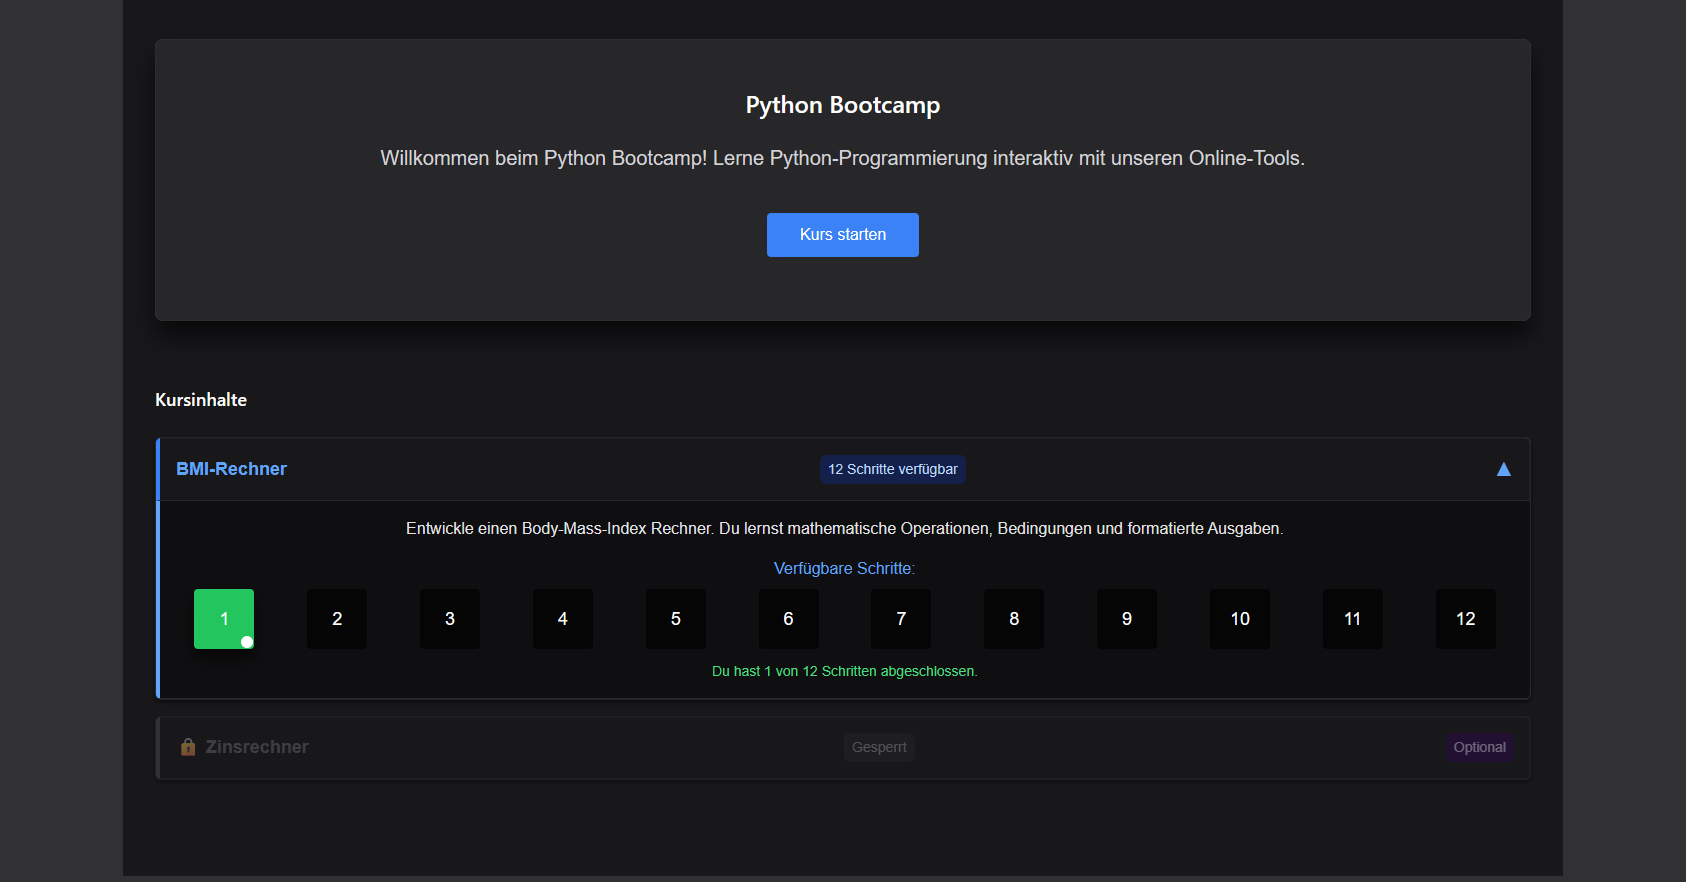
\includegraphics[width=0.80\textwidth]{pic/bilder-der-app/home-kursuebersicht}
    \caption{Dashboard mit Kursübersicht. Abgeschlossene Schritte werden grün hervorgehoben; der Zinsrechner ist als optionaler Aufbaukurs gesperrt, bis der BMI-Rechner abgeschlossen wurde.}
    \label{fig:anhang_dashboard}
\end{figure}

\begin{figure}[htbp]
    \centering
    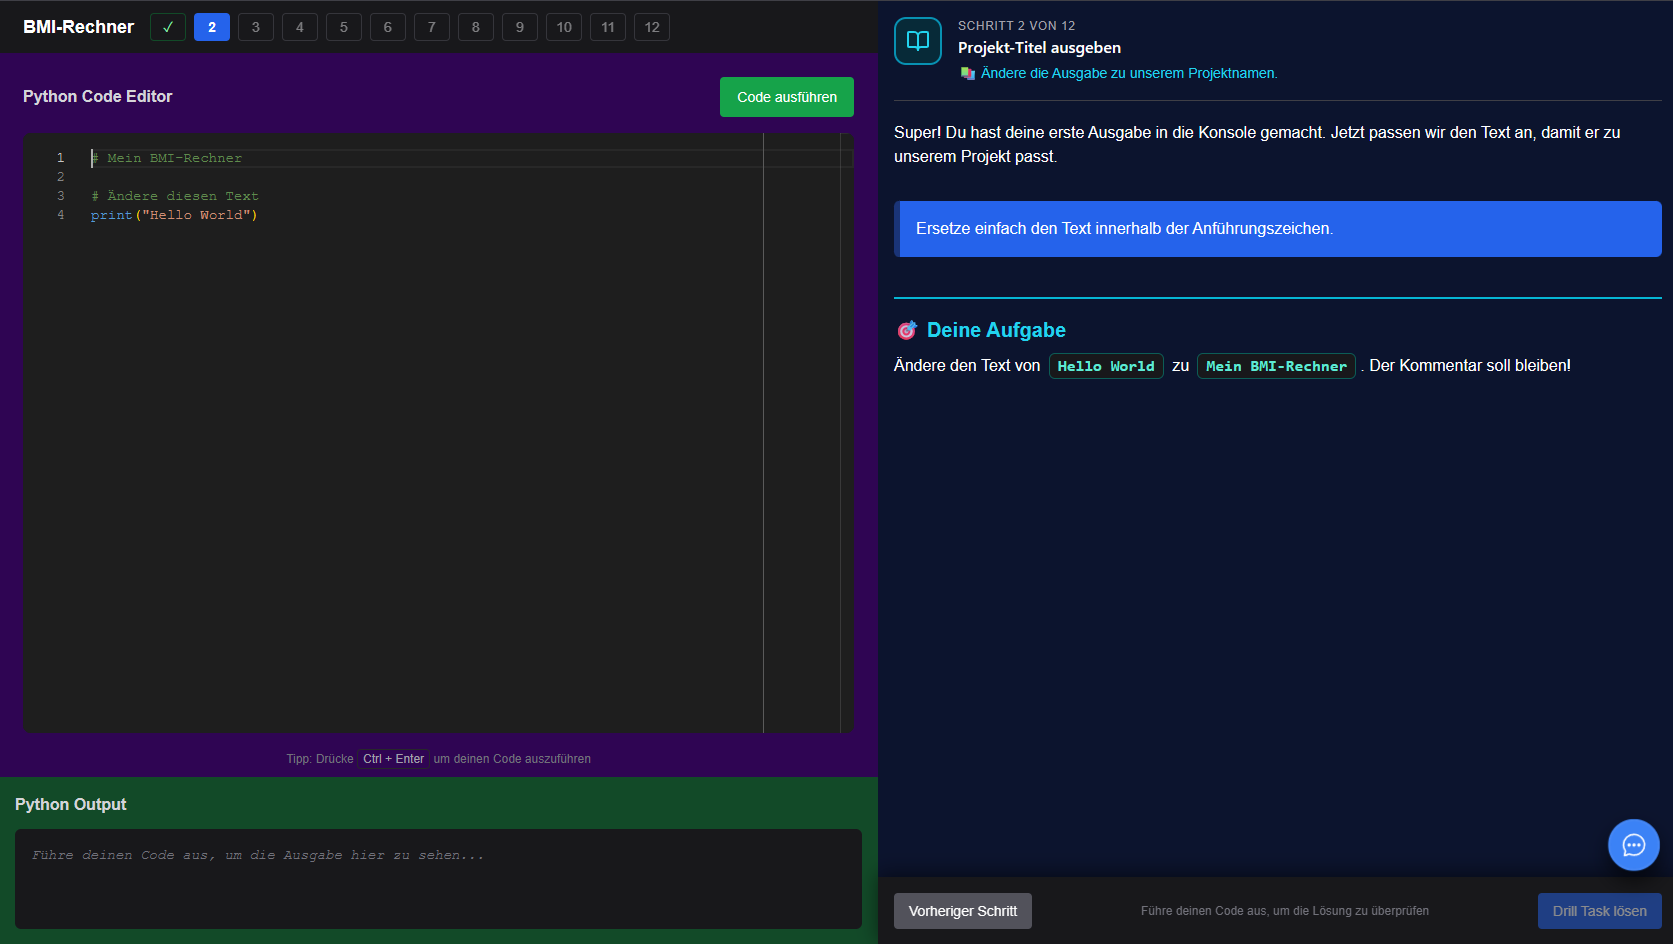
\includegraphics[width=0.75\textwidth]{pic/bilder-der-app/kursansicht-full}
    \caption{Kursansicht (Schritt~1 von 12): Links der Monaco-Code-Editor mit Startercode und Python-Ausgabebereich, rechts die Aufgabenstellung mit farbigen Hinweisboxen. Der blaue Chat-Button (roter Pfeil) öffnet den KI-Tutor (nur Gruppe~B).}
    \label{fig:anhang_kursansicht}
\end{figure}

\begin{figure}[htbp]
    \centering
    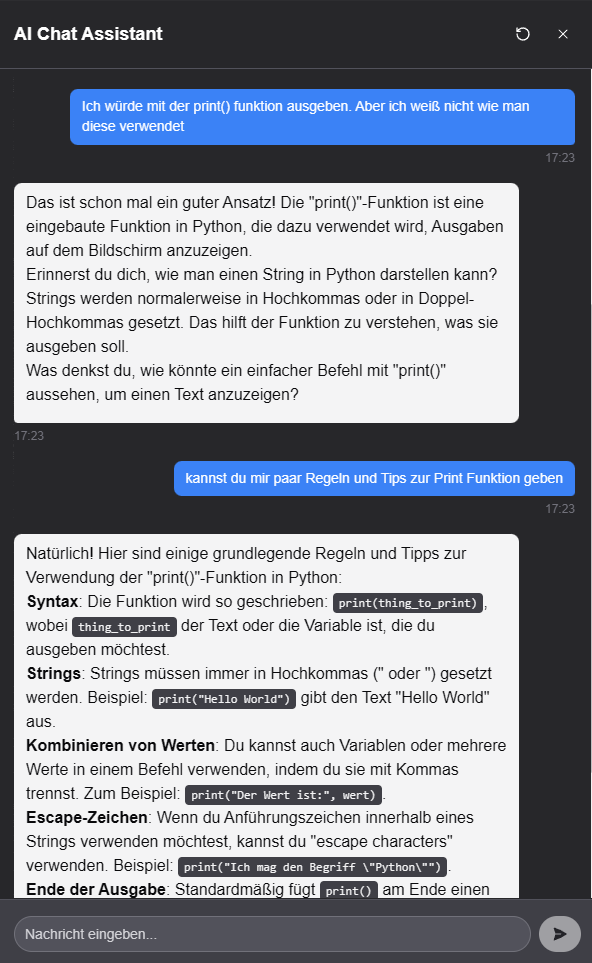
\includegraphics[width=0.75\textwidth]{pic/bilder-der-app/chat-beispiel}
    \caption{KI-Tutor-Chat (Gruppe~B): Das progressive Hint-System antwortet auf eine Frage zur \texttt{print()}-Funktion mit Rückfragen statt direkter Lösung.}
    \label{fig:anhang_chatverlaeufe}
\end{figure}

\begin{figure}[htbp]
    \centering
    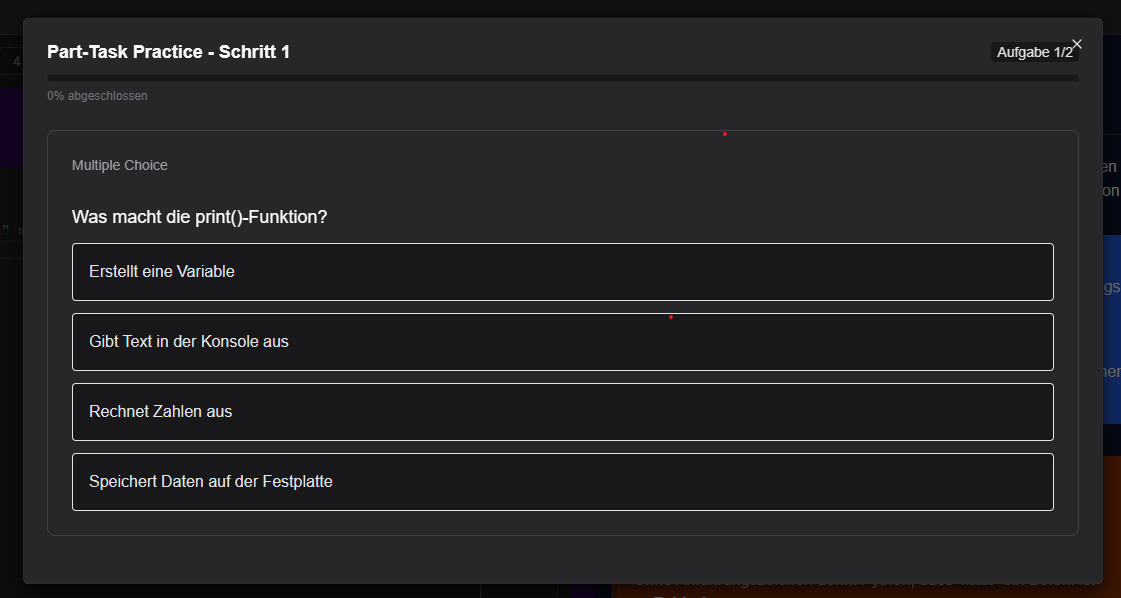
\includegraphics[width=0.75\textwidth]{pic/bilder-der-app/drill-multiple-choice}
    \caption{Part-task Practice -- Multiple-Choice-Aufgabe (Schritt~1): Konzeptabfrage zur \texttt{print()}-Funktion aus dem statischen Drill-Pool.}
    \label{fig:anhang_drill_mcq}
\end{figure}

\begin{figure}[htbp]
    \centering
    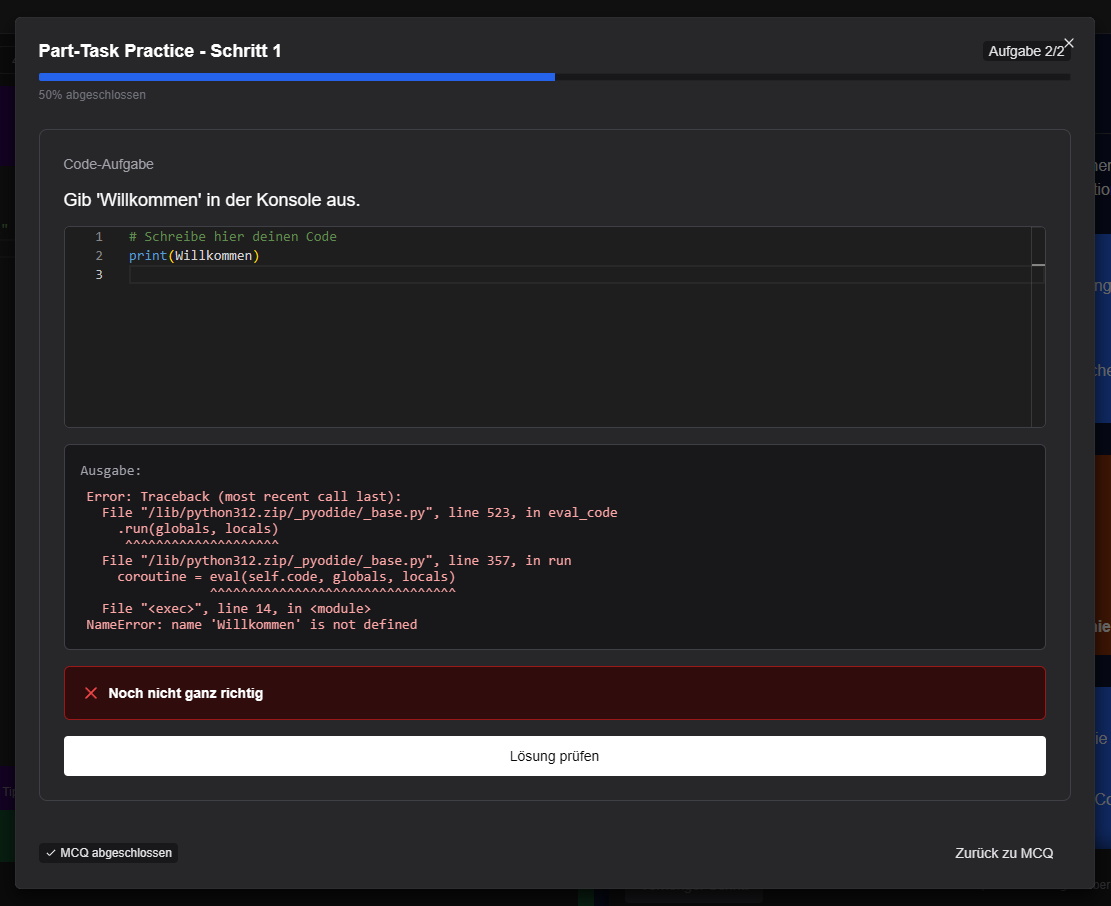
\includegraphics[width=0.75\textwidth]{pic/bilder-der-app/drill-code-aufgabe}
    \caption{Part-task Practice -- Code-Aufgabe (Schritt~1): Die Lernende hat \texttt{Willkommen} ohne Anführungszeichen eingegeben; das System zeigt den Python-Fehler und meldet die Lösung als noch nicht korrekt.}
    \label{fig:anhang_drill_code}
\end{figure}

\clearpage
\section*{E: Werkzeug- und KI-Protokoll}

Nachfolgend sind alle wesentlichen digitalen Werkzeuge und KI-Systeme aufgeführt, die bei der Erstellung dieser Arbeit zum Einsatz kamen.
Die Auflistung folgt der Empfehlung des Betreuers, alle verwendeten Hilfsmittel transparent auszuweisen.

\renewcommand{\arraystretch}{1.4}
\begin{table}[htbp]
\centering
\caption{Protokoll der verwendeten Werkzeuge und KI-Systeme}
\label{tab:werkzeugprotokoll}
% reduce inter-column padding and slightly smaller font to help fit columns
\begingroup
	\setlength{\tabcolsep}{6pt}% adjust if necessary
	\small
	\begin{tabular}{|P{3.2cm}|P{2.6cm}|P{4.6cm}|P{3.8cm}|}
	\hline
	\textbf{Werkzeug / System} & \textbf{Version / Zeitraum} & \textbf{Einsatzbereich} & \textbf{Validierung} \\
	\hline
	GitHub Copilot (Microsoft) mit GPT-4o, GPT-5.1 sowie Claude~Sonnet~4.6 \& Claude~Opus~4.6 (Anthropic) &
	Copilot in VS~Code, Juni~2025--Mrz.~2026 &
	Formulierungsvorschläge, Gliederungsstruktur, \LaTeX-Syntax, Erarbeitung von Kapitelgerüsten und Leitfragen, Code-Generierung und -Analyse, BibTeX-Bereinigung; KI-Unterstützung bei der Entwicklung der Lernplattform-Codebase &
	Alle Ausgaben manuell geprüft und inhaltlich angepasst; Quellen und DOIs separat veri\-fiziert \\
	\hline
	Visual Studio Code \cite{vscode} mit LaTeX Workshop Extension &
	VS~Code~1.x, Feb.--Mrz.~2026 &
	Entwicklungsumgebung für \LaTeX-Ausarbeitung und Programmierprototyp; Build, Formatierung, PDF-Vorschau &
	Kein KI-Einsatz; reines Editierwerkzeug \\
	\hline
	latexmk / \TeX~Live (WSL) &
	\TeX~Live~2024, Feb.--Mrz.~2026 &
	Kompilierung der \LaTeX-Arbeit zu PDF &
	Kein KI-Einsatz \\
	\hline
	OpenAI API (gpt-4o-mini) \cite{openai_api} &
	API, Jan.--Mrz.~2026 &
	KI-Tutor und Aufgabenauswahl im entwickelten Lernprototyp (Forschungsgegenstand der Arbeit) &
	Prototyp-intern; Ausgaben im Rahmen der Studie erhoben und ausgewertet \\
	\hline
	\end{tabular}
\endgroup
\end{table}

\noindent
\textit{Anmerkung:} Triviale Werkzeuge (Browser, Datei\-ver\-wal\-tung) sind gemäß den Hinweisen des Betreuers nicht gesondert aufgeführt.
Die inhaltliche Verantwortung für alle Aussagen, Interpretationen und Schlussfolgerungen liegt beim Autor.

\end{document}
